% !TeX spellcheck = hu_HU
% !TeX encoding = UTF-8
% !TeX program = xelatex
\documentclass[11pt,a4paper,oneside]{report}

% thanks to http://tex.stackexchange.com/a/47579/71109
\usepackage{ifxetex}
\usepackage{ifluatex}
\newif\ifxetexorluatex % a new conditional starts as false
\ifnum 0\ifxetex 1\fi\ifluatex 1\fi>0
  \xetexorluatextrue
\fi

\ifxetexorluatex
  \usepackage{fontspec}
\else
  \usepackage[T1]{fontenc}
  \usepackage[utf8]{inputenc}
  \usepackage[lighttt]{lmodern}
\fi

\usepackage[english,magyar]{babel} % Alapértelmezés szerint utoljára definiált nyelv lesz aktív, de később külön beállítjuk az aktív nyelvet.

%\usepackage{cmap}
\usepackage{amsfonts,amsmath,amssymb} % Mathematical symbols.
%\usepackage[ruled,boxed,resetcount,linesnumbered]{algorithm2e} % For pseudocodes. % beware: this is not compatible with LuaLaTeX, see http://tex.stackexchange.com/questions/34814/lualatex-and-algorithm2e
\usepackage{booktabs} % For publication quality tables for LaTeX
\usepackage{graphicx}

%\usepackage{fancyhdr}
%\usepackage{lastpage}

\usepackage{anysize}
%\usepackage{sectsty}
\usepackage{setspace} % For setting line spacing

\usepackage[unicode]{hyperref} % For hyperlinks in the generated document.
\usepackage{xcolor}
\usepackage{listings} % For source code snippets.

\usepackage[amsmath,thmmarks]{ntheorem} % Theorem-like environments.

\usepackage[hang]{caption}

\newcommand{\selecthungarian}{
  \selectlanguage{magyar}
  \setlength{\parindent}{2em}
  \setlength{\parskip}{0em}
  \frenchspacing
}

\newcommand{\selectenglish}{
  \selectlanguage{english}
  \setlength{\parindent}{0em}
  \setlength{\parskip}{0.5em}
  \nonfrenchspacing
  \renewcommand{\figureautorefname}{Figure}
  \renewcommand{\tableautorefname}{Table}
  \renewcommand{\partautorefname}{Part}
  \renewcommand{\chapterautorefname}{Chapter}
  \renewcommand{\sectionautorefname}{Section}
  \renewcommand{\subsectionautorefname}{Section}
  \renewcommand{\subsubsectionautorefname}{Section}
}

\usepackage[numbers]{natbib}
\usepackage{xspace}

\usepackage{xurl} % For breaking long URLs in the bibliography.

% js listing
\usepackage{listings}
\usepackage[many]{tcolorbox}
\usepackage{xcolor}

% colors
\definecolor{white}{rgb}{1,1,1}
\definecolor{black}{rgb}{0,0,0}
\definecolor{middlegray}{rgb}{0.5,0.5,0.5}
\definecolor{lightgray}{rgb}{.95,.95,.95}
\definecolor{arsenic}{rgb}{0.23, 0.27, 0.29}
\definecolor{arsenicLight}{rgb}{0.20, 0.20, 0.20}
\definecolor{darkgray}{rgb}{.4,.4,.4}
\definecolor{purple}{rgb}{0.65, 0.12, 0.82}
\definecolor{orange}{rgb}{0.8,0.3,0.3}
\definecolor{yac}{rgb}{0.6,0.6,0.1}
\definecolor{green}{rgb}{.2,0.6,0.3}
\definecolor{azure}{rgb}{0.0, 0.5, 1.0}
\definecolor{editorGray}{rgb}{0.95, 0.95, 0.95}
\definecolor{editorOcher}{rgb}{1, 0.5, 0}
\definecolor{editorGreen}{rgb}{0, 0.5, 0}
\definecolor{orange}{rgb}{1,0.45,0.13}
\definecolor{olive}{rgb}{0.17,0.59,0.20}
\definecolor{brown}{rgb}{0.69,0.31,0.31}
\definecolor{purple}{rgb}{0.38,0.18,0.81}
\definecolor{lightblue}{rgb}{0.1,0.57,0.7}
\definecolor{lightred}{rgb}{1,0.4,0.5}
\definecolor{amber}{rgb}{1.0, 0.75, 0.0}

\definecolor{vscodered}{HTML}{E53935}
\definecolor{vscodelightred}{HTML}{EF5350}
\definecolor{vscodeblue}{HTML}{1565C0}
\definecolor{vscodegreen}{HTML}{66BB6A}

\definecolor{lightblack}{HTML}{212121}
\definecolor{darkraspberry}{rgb}{0.53, 0.15, 0.34}

% blue hues
\definecolor{bleudefrance}{rgb}{0.19, 0.55, 0.91}
\definecolor{brandeisblue}{rgb}{0.0, 0.44, 1.0}
\definecolor{blue(ncs)}{rgb}{0.0, 0.53, 0.74}
\definecolor{coolblack}{rgb}{0.0, 0.18, 0.39}

% red hues
\definecolor{coralred}{rgb}{1.0, 0.25, 0.25}
\definecolor{darkred}{rgb}{0.55, 0.0, 0.0}

% general settings for listing
\lstset{
basicstyle=\normalsize\ttfamily,
basewidth  = {.5em,0.4em},
captionpos=t,
lineskip={2pt},
backgroundcolor=\color{white},
framextopmargin=6pt,
framexrightmargin=0.9em,
framexleftmargin=0.9em,
framexbottommargin=6pt,
frame=tb,
framerule=0pt,
framesep=6.5mm,
fillcolor=\color{white},
rulecolor=\color{middlegray},
numbers=left,
numberstyle=\normalfont\color{middlegray},
numbersep=16pt,
abovecaptionskip=-5pt, %space above the caption
belowcaptionskip=10pt, %space below the caption
extendedchars=true,
showstringspaces=false,
showspaces=false,
stepnumber=1, % the step between two line-numbers. If it is 1 each line will be numbered
tabsize=2,
breaklines=true,
showtabs=false,
upquote=true,
% German umlauts
literate=%
  {Ö}{{\"O}}1
{Ä}{{\"A}}1
{Ü}{{\"U}}1
{ß}{{\ss}}1
{ü}{{\"u}}1
{ä}{{\"a}}1
{ö}{{\"o}}1
}

% define language
\lstdefinelanguage{JavaScript}{
  keywords={typeof, new, true, false, catch, then, function, return, catch, switch, var, if, in, while, do, else, case, break, default, this, process},
  keywordstyle=\color{editorGreen}\bfseries,
  ndkeywords={class, export, boolean, throw, implements, import, from, const, async, await, private, public, readonly, static, constructor, get, set, yield, interface, type},
  ndkeywordstyle=\color{vscodeblue}\bfseries,
  identifierstyle=\color{black},
  sensitive=false,
  comment=[l]{//},
  morecomment=[s]{/*}{*/},
  commentstyle=\color{editorGreen}\ttfamily,
  stringstyle=\color{darkred}\ttfamily,
  morestring=[b]',
  morestring=[b]",
  morestring=*[d]`,
  moredelim=[s][]{\$\{}{\}},
  morekeywords=[3]{@UseGuards, @ApiFoundResponse, @ApiQuery, @Controller, @Injectable, @Module, @Inject, @Body, @Param, @Query, @UseInterceptors, @UseFilters, @UploadedFile, @UsePipes, @Get, @Post, @Put, @Delete, @Patch, @CurrentUser, @Res, @Next, @Headers, @Session, @Request, @All, string, number, null, void, undefined},
  keywordstyle={[3]\color{darkraspberry}\bfseries}
}

\lstdefinelanguage{SQL}{
  keywords={select, where, from},
  keywordstyle=\color{editorGreen}\bfseries,
  ndkeywords={},
  ndkeywordstyle=\color{vscodeblue}\bfseries,
  identifierstyle=\color{black},
  sensitive=false,
  comment=[l]{--},
  morecomment=[s]{/*}{*/},
  commentstyle=\color{editorGreen}\ttfamily,
  stringstyle=\color{darkred}\ttfamily,
  morestring=[b]',
  morestring=[b]"
}


\lstdefinelanguage{HTML5}{
  language=html,
  sensitive=true,
  alsoletter={<>=-},
  morecomment=[s]{<!-}{-->},
  tag=[s],
  otherkeywords={
      % General
      >,
      % Standard tags
      <!DOCTYPE,
      </html, <html, <head, <title, </title, <style, </style, <link, </head, <meta, />,
      % body
      </body, <body,
      % Divs
      </div, <div, </div>,
      % Paragraphs
      </p, <p, </p>,
      % scripts
      </script, <script,
      % More tags...
      <canvas, /canvas>, <svg, <rect, <animateTransform, </rect>, </svg>, <video, <source, <iframe, </iframe>, </video>, <image, </image>, <header, </header, <article, </article
    },
  ndkeywords={
      % General
      =,
      % HTML attributes
      charset=, src=, id=, width=, height=, style=, type=, rel=, href=,
      % SVG attributes
      fill=, attributeName=, begin=, dur=, from=, to=, poster=, controls=, x=, y=, repeatCount=, xlink:href=,
      % properties
      margin:, padding:, background-image:, border:, top:, left:, position:, width:, height:, margin-top:, margin-bottom:, font-size:, line-height:,
      % CSS3 properties
      transform:, -moz-transform:, -webkit-transform:,
      animation:, -webkit-animation:,
      transition:,  transition-duration:, transition-property:, transition-timing-function:,
    }
}

\lstdefinelanguage{Terraform}{
  keywords={terraform, variable, locals, output, module, resource, data, backend, true, false, var, local},
  keywordstyle=\color{vscodegreen}\bfseries,
  ndkeywords={lifecycle, provisioner, connection, length, lookup, merge, coalesce, zipmap, flatten, try, null, for, if, else, each, in, template_file, object, map, string, number, null_resource},
  ndkeywordstyle=\color{vscodeblue}\bfseries,
  sensitive=false,
  comment=[l]{\#},
  commentstyle=\color{editorGreen}\ttfamily,
  stringstyle=\color{darkred}\ttfamily,
  moredelim=[s][]{\$\{}{\}},
  morestring=[b]',
  morestring=*[d]",
  identifierstyle=\color{black}\ttfamily,
}

\lstdefinelanguage{Dockerfile}{
  keywords={FROM, RUN, COPY, ADD, ENTRYPOINT, CMD,  ENV, ARG, WORKDIR, EXPOSE, LABEL, USER, VOLUME, STOPSIGNAL, ONBUILD, MAINTAINER, HEALTHCHECK},
  keywordstyle=\color{vscodeblue}\bfseries,
  identifierstyle=\color{black},
  sensitive=false,
  comment=[l]{\#},
  commentstyle=\color{editorGreen}\ttfamily,
  stringstyle=\color{darkred}\ttfamily,
  morestring=[b]',
  morestring=[b]"
}

\lstdefinestyle{html} {%
% Code design
keywordstyle=\color{lightblack}\bfseries,
ndkeywordstyle=\color{lightblack}\bfseries,
identifierstyle=\color{lightblack},
commentstyle=\color{green}\ttfamily,
stringstyle=\color{darkred}\ttfamily,
% Code
language=HTML5,
%  alsolanguage=JavaScript,
alsodigit={.:;},
tabsize=2,
showtabs=false,
showspaces=false,
showstringspaces=false,
extendedchars=true,
breaklines=true,
% German umlauts
literate=%
  {Ö}{{\"O}}1
{Ä}{{\"A}}1
{Ü}{{\"U}}1
{ß}{{\ss}}1
{ü}{{\"u}}1
{ä}{{\"a}}1
{ö}{{\"o}}1
}

\lstdefinelanguage{CSS}
{morekeywords={color,background,margin,padding,margin,padding,font,weight,display,position,top,left,right,bottom,list,style,border,size,white,space,min,width, 	transition},
  sensitive=false,
  morecomment=[l]{//},
  morecomment=[s]{/*}{*/},
  morestring=[b]",
}

\newcommand\YAMLcolonstyle{\color{darkred}\mdseries}
\newcommand\YAMLkeystyle{\color{black}\bfseries}
\newcommand\YAMLvaluestyle{\color{vscodeblue}\mdseries}

\lstdefinelanguage{YAML}{
  keywords={true,false,null,y,n},
  keywordstyle=\color{darkgray}\bfseries,
  basicstyle=\YAMLkeystyle,                                 % assuming a key comes first
  sensitive=false,
  comment=[l]{\#},
  morecomment=[s]{/*}{*/},
  commentstyle=\color{editorGreen}\ttfamily,
  stringstyle=\YAMLvaluestyle\ttfamily,
  % moredelim=[l][\color{orange}]{\&},
  moredelim=[l][\color{magenta}]{*},
  moredelim=**[il][\YAMLcolonstyle{:}\YAMLvaluestyle]{:},   % switch to value style at :
  morestring=[b]',
  morestring=[b]",
  literate =    {---}{{\ProcessThreeDashes}}3
  {>}{{\textcolor{red}\textgreater}}1
  {|}{{\textcolor{red}\textbar}}1
  {\ -\ }{{\mdseries\ -\ }}3,
}

\lstdefinestyle{css} {
  language=CSS,
  keywordstyle=\color{lightblack},
}

\lstdefinestyle{js} {
  language=JavaScript
}

\lstdefinestyle{tf} {
  language=Terraform
}

\lstdefinestyle{dockerfile} {
  language=Dockerfile
}

\lstdefinestyle{yaml} {
  language=YAML
}

\lstdefinestyle{sql} {
  language=SQL,
  keywordstyle=\color{azure}
}

% Hyphenation rules
\hyphenation{PostgreSQL Cloud-Front strea-ming stream pa-cket Apple Lambda Edge Route Node Vite Actions Action Type-Script Java-Script-ből Java-Script React Function Rou-ter route table build buil-del Re-quest bucket re-po-si-to-ry Docker Registry Se-cu-ri-ty Group Gate-way Cloud-Watch AuthSCH OAuth Chrome Google Media-Package Media-Live back-end front-end}


\onehalfspacing % Set line spacing to 1.5

\newcommand{\vikszerzoVezeteknev}{Piller}
\newcommand{\vikszerzoKeresztnev}{Trisztán}

\newcommand{\vikkonzulensAMegszolitas}{}
\newcommand{\vikkonzulensAVezeteknev}{Kövesdán}
\newcommand{\vikkonzulensAKeresztnev}{Gábor}

\newcommand{\vikkonzulensBMegszolitas}{}
\newcommand{\vikkonzulensBVezeteknev}{}
\newcommand{\vikkonzulensBKeresztnev}{}

\newcommand{\vikkonzulensCMegszolitas}{}
\newcommand{\vikkonzulensCVezeteknev}{}
\newcommand{\vikkonzulensCKeresztnev}{}

\newcommand{\vikcim}{Videó streaming szolgáltatások implementációja}
\newcommand{\viktanszek}{\bmeaut} 
\newcommand{\vikdoktipus}{\msc}
\newcommand{\vikmunkatipusat}{diplomatervet} 

%--------------------------------------------------------------------------------------
% TDK-specifikus változók
%--------------------------------------------------------------------------------------
\newcommand{\tdkszerzoB}{Második Szerző} % Második szerző neve; hagyd üresen, ha egyedül írtad a TDK-t.
\newcommand{\tdkev}{2014} % A dolgozat írásának éve (pl. "2014") (Ez OTDK-nál eltérhet az aktuális évtől.)

% További adatok az OTDK címlaphoz (BME-s TDK-hoz nem kell kitölteni)
\newcommand{\tdkevfolyamA}{IV} % Első szerző évfolyama, római számmal (pl. IV).
\newcommand{\tdkevfolyamB}{III} % Második szerző évfolyama, római számmal (pl. III).
\newcommand{\tdkkonzulensbeosztasA}{egyetemi tanár} % Első konzulens beosztása (pl. egyetemi docens)
\newcommand{\tdkkonzulensbeosztasB}{doktorandusz} % Második konzulens beosztása (pl. egyetemi docens)

\newcommand{\szerzoMeta}{\vikszerzoVezeteknev{} \vikszerzoKeresztnev} 

%--------------------------------------------------------------------------------------
% Elnevezések
%--------------------------------------------------------------------------------------
\newcommand{\bme}{Budapesti Műszaki és Gazdaságtudományi Egyetem}
\newcommand{\vik}{Villamosmérnöki és Informatikai Kar}

\newcommand{\bmemit}{Méréstechnika és Információs Rendszerek Tanszék}
\newcommand{\bmeaut}{Automatizálási és Alkalmazott Informatikai Tanszék}

\newcommand{\keszitette}{Készítette}
\newcommand{\konzulens}{Konzulens}

\newcommand{\bsc}{Szakdolgozat}
\newcommand{\msc}{Diplomaterv}
\newcommand{\tdk}{TDK dolgozat}
\newcommand{\bsconlab}{BSc Önálló laboratórium}
\newcommand{\msconlabi}{MSc Önálló laboratórium 1.}
\newcommand{\msconlabii}{MSc Önálló laboratórium 2.}

\newcommand{\pelda}{Példa}
\newcommand{\definicio}{Definíció}
\newcommand{\tetel}{Tétel}

\newcommand{\bevezetes}{Bevezetés}
\newcommand{\koszonetnyilvanitas}{Köszönetnyilvánítás}
\newcommand{\fuggelek}{Függelék}

% Opcionálisan átnevezhető címek
%\addto\captionsmagyar{%
%\renewcommand{\listfigurename}{Saját ábrajegyzék cím}
%\renewcommand{\listtablename}{Saját táblázatjegyzék cím}
%\renewcommand{\bibname}{Saját irodalomjegyzék név}
%}

\newcommand{\szerzo}{\vikszerzoVezeteknev{} \vikszerzoKeresztnev}
\newcommand{\vikkonzulensA}{\vikkonzulensAMegszolitas\vikkonzulensAVezeteknev{} \vikkonzulensAKeresztnev}
\newcommand{\vikkonzulensB}{\vikkonzulensBMegszolitas\vikkonzulensBVezeteknev{} \vikkonzulensBKeresztnev}
\newcommand{\vikkonzulensC}{\vikkonzulensCMegszolitas\vikkonzulensCVezeteknev{} \vikkonzulensCKeresztnev}

\newcommand{\selectthesislanguage}{\selecthungarian}

\bibliographystyle{huplain}

\def\lstlistingname{lista}

\newcommand{\appendixnumber}{6}  % a fofejezet-szamlalo az angol ABC 6. betuje (F) lesz

%--------------------------------------------------------------------------------------
% Page layout setup
%--------------------------------------------------------------------------------------
% we need to redefine the pagestyle plain
% another possibility is to use the body of this command without \fancypagestyle
% and use \pagestyle{fancy} but in that case the special pages
% (like the ToC, the References, and the Chapter pages)remain in plane style

\pagestyle{plain}
\marginsize{35mm}{25mm}{15mm}{15mm}

\setcounter{tocdepth}{3}
%\sectionfont{\large\upshape\bfseries}
\setcounter{secnumdepth}{3}

\sloppy % Margón túllógó sorok tiltása.
\widowpenalty=10000 \clubpenalty=10000 %A fattyú- és árvasorok elkerülése
\def\hyph{-\penalty0\hskip0pt\relax} % Kötőjeles szavak elválasztásának engedélyezése


%--------------------------------------------------------------------------------------
% Setup hyperref package
%--------------------------------------------------------------------------------------
\hypersetup{
    % bookmarks=true,            % show bookmarks bar?
    unicode=true,              % non-Latin characters in Acrobat's bookmarks
    pdftitle={\vikcim},        % title
    pdfauthor={\szerzoMeta},    % author
    pdfsubject={\vikdoktipus}, % subject of the document
    pdfcreator={\szerzoMeta},   % creator of the document
    pdfproducer={},    % producer of the document
    pdfkeywords={},    % list of keywords (separate then by comma)
    pdfnewwindow=true,         % links in new window
    colorlinks=true,           % false: boxed links; true: colored links
    linkcolor=black,           % color of internal links
    citecolor=black,           % color of links to bibliography
    filecolor=black,           % color of file links
    urlcolor=black             % color of external links
}


%--------------------------------------------------------------------------------------
% Set up listings
%--------------------------------------------------------------------------------------
\definecolor{lightgray}{rgb}{0.95,0.95,0.95}
\lstset{
	basicstyle=\scriptsize\ttfamily, % print whole listing small
	keywordstyle=\color{black}\bfseries, % bold black keywords
	identifierstyle=, % nothing happens
	% default behavior: comments in italic, to change use
	% commentstyle=\color{green}, % for e.g. green comments
	stringstyle=\scriptsize,
	showstringspaces=false, % no special string spaces
	aboveskip=3pt,
	belowskip=3pt,
	backgroundcolor=\color{lightgray},
	columns=flexible,
	keepspaces=true,
	escapeinside={(*@}{@*)},
	captionpos=b,
	breaklines=true,
	frame=single,
	float=!ht,
	tabsize=2,
	literate=*
		{á}{{\'a}}1	{é}{{\'e}}1	{í}{{\'i}}1	{ó}{{\'o}}1	{ö}{{\"o}}1	{ő}{{\H{o}}}1	{ú}{{\'u}}1	{ü}{{\"u}}1	{ű}{{\H{u}}}1
		{Á}{{\'A}}1	{É}{{\'E}}1	{Í}{{\'I}}1	{Ó}{{\'O}}1	{Ö}{{\"O}}1	{Ő}{{\H{O}}}1	{Ú}{{\'U}}1	{Ü}{{\"U}}1	{Ű}{{\H{U}}}1
}


%--------------------------------------------------------------------------------------
% Set up theorem-like environments
%--------------------------------------------------------------------------------------
% Using ntheorem package -- see http://www.math.washington.edu/tex-archive/macros/latex/contrib/ntheorem/ntheorem.pdf

\theoremstyle{plain}
\theoremseparator{.}
\newtheorem{example}{\pelda}

\theoremseparator{.}
%\theoremprework{\bigskip\hrule\medskip}
%\theorempostwork{\hrule\bigskip}
\theorembodyfont{\upshape}
\theoremsymbol{{\large \ensuremath{\centerdot}}}
\newtheorem{definition}{\definicio}

\theoremseparator{.}
%\theoremprework{\bigskip\hrule\medskip}
%\theorempostwork{\hrule\bigskip}
\newtheorem{theorem}{\tetel}


%--------------------------------------------------------------------------------------
% Some new commands and declarations
%--------------------------------------------------------------------------------------
\newcommand{\code}[1]{{\upshape\ttfamily\scriptsize\indent #1}}
\newcommand{\doi}[1]{DOI: \href{http://dx.doi.org/\detokenize{#1}}{\raggedright{\texttt{\detokenize{#1}}}}} % A hivatkozások közt így könnyebb DOI-t megadni.

\DeclareMathOperator*{\argmax}{arg\,max}
%\DeclareMathOperator*[1]{\floor}{arg\,max}
\DeclareMathOperator{\sign}{sgn}
\DeclareMathOperator{\rot}{rot}


%--------------------------------------------------------------------------------------
% Setup captions
%--------------------------------------------------------------------------------------
\captionsetup[figure]{
	width=.75\textwidth,
	aboveskip=10pt}

\renewcommand{\captionlabelfont}{\bf}
%\renewcommand{\captionfont}{\footnotesize\it}

%--------------------------------------------------------------------------------------
% Hyphenation exceptions
%--------------------------------------------------------------------------------------
\hyphenation{Shakes-peare Mar-seilles ár-víz-tű-rő tü-kör-fú-ró-gép}


\author{\vikszerzo}
\title{\viktitle}

\begin{document}

\pagenumbering{gobble}

% %--------------------------------------------------------------------------------------
% Feladatkiiras (a tanszeken atveheto, kinyomtatott valtozat)
%--------------------------------------------------------------------------------------
\clearpage
\begin{center}
\large
\textbf{FELADATKIÍRÁS}\\
\end{center}

A feladatkiírást a tanszéki adminisztrációban lehet átvenni, és a leadott munkába eredeti, tanszéki pecséttel ellátott és a tanszékvezető által aláírt lapot kell belefűzni (ezen oldal \emph{helyett}, ez az oldal csak útmutatás). Az elektronikusan feltöltött dolgozatban már nem kell beleszerkeszteni ezt a feladatkiírást.


\selectthesislanguage
\hypersetup{pageanchor=false}
%--------------------------------------------------------------------------------------
%	The title page
%--------------------------------------------------------------------------------------
\begin{titlepage}
\begin{center}

\includegraphics[width=60mm,keepaspectratio]{figures/bme_logo.pdf}\\
\vspace{0.3cm}
\textbf{\bme}\\
\textmd{\vik}\\
\textmd{\viktanszek}\\[5cm]

\vspace{0.4cm}
{\huge \bfseries \vikcim}\\[0.8cm]
\vspace{0.5cm}
\textsc{\Large \vikdoktipus}\\[4cm]

{
	\renewcommand{\arraystretch}{0.85}
	\begin{tabular}{cc}
	 \makebox[7cm]{\emph{\keszitette}} & \makebox[7cm]{\emph{\konzulens}} \\ \noalign{\smallskip}
	 \makebox[7cm]{\szerzo} & \makebox[7cm]{\vikkonzulensA} \\
	  & \makebox[7cm]{\vikkonzulensB} \\
	  & \makebox[7cm]{\vikkonzulensC} \\
	\end{tabular}
}

\vfill
{\large \today}
\end{center}
\end{titlepage}
\hypersetup{pageanchor=false}

	

\singlespacing % Set line spacing to 1
\tableofcontents\vfill

\onehalfspacing % Set line spacing to 1.5

\selectlanguage{magyar}
\pagenumbering{gobble}
%--------------------------------------------------------------------------------------
% Nyilatkozat
%--------------------------------------------------------------------------------------
\begin{center}
\large
\textbf{HALLGATÓI NYILATKOZAT}\\
\end{center}

Alulírott \emph{\vikszerzoVezeteknev{} \vikszerzoKeresztnev}, szigorló hallgató kijelentem, hogy ezt a \vikmunkatipusat{} meg nem engedett segítség nélkül, saját magam készítettem, csak a megadott forrásokat (szakirodalom, eszközök stb.) használtam fel. Minden olyan részt, melyet szó szerint, vagy azonos értelemben, de átfogalmazva más forrásból átvettem, egyértelműen, a forrás megadásával megjelöltem.

Hozzájárulok, hogy a jelen munkám alapadatait (szerző(k), cím, angol és magyar nyelvű tartalmi kivonat, készítés éve, konzulens(ek) neve) a BME VIK nyilvánosan hozzáférhető elektronikus formában, a munka teljes szövegét pedig az egyetem belső hálózatán keresztül (vagy autentikált felhasználók számára) közzétegye. Kijelentem, hogy a benyújtott munka és annak elektronikus verziója megegyezik. Dékáni engedéllyel titkosított diplomatervek esetén a dolgozat szövege csak 3 év eltelte után válik hozzáférhetővé.

\begin{flushleft}
\vspace*{1cm}
Budapest, \today
\end{flushleft}

\begin{flushright}
 \vspace*{1cm}
 \makebox[7cm]{\rule{6cm}{.4pt}}\\
 \makebox[7cm]{\emph{\vikszerzoVezeteknev{} \vikszerzoKeresztnev}}\\
 \makebox[7cm]{hallgató}
\end{flushright}
\thispagestyle{empty}

\vfill
\clearpage
\thispagestyle{empty} % an empty page

\selectthesislanguage

\pagenumbering{roman}
\setcounter{page}{1}

\selecthungarian

%----------------------------------------------------------------------------
% Abstract in Hungarian
%----------------------------------------------------------------------------
\chapter*{Kivonat}\addcontentsline{toc}{chapter}{Kivonat}

Az IT szakma meghatározó kihívása a magasan teljesítőképes, könnyen skálázódó és stabil infrastruktúra létesítése különféle üzleti célok megvalósítására. A hírközlés, a média és a szórakoztatatás iparágaiban is kiemelt figyelmet kap ez a kihívás.

Ezek a virágzó és feltörekvő iparágak folyamatosan igénylik az olyan szoftverfejlesztőket, akik ezekre az iparágakra specializáltan is folyamatosan képzik magukat, valamint mélyen ismerik a szakterület technológiáit.

Diplomatervem célja demonstrálni egy az Amazon Web Services platformján futó felhő alapú médiaszolgáltatás-rendszer alapos tervezésének, implementálásának, valamint tesztelésének folyamatát. A rendszer a videó streaming szolgáltatások területén nyújt weben elérhető megoldást, és a felhasználók számára lehetővé teszi, hogy saját időbeosztásuknak megfelelően férjenek hozzá videótartalmakhoz (Video-on-Demand), valami élő adásokat is tudjanak megtekinteni (live streaming).

A megoldás ismertetése során kiemelt fókuszt kap a komponensek közötti laza kapcsolás kialakítása, az IT biztonsági kockázatok kezelése, az konfigurációmenedzsment fenntarthatósága. Felhasználásra kerülnek modern webes technológiák és DevOps technikák, mint a konténerizáció, a serverless függvények, a CI/CD csővezetékek és az Infrastructure as Code.

\vfill
\selectenglish

%----------------------------------------------------------------------------
% Abstract in English
%----------------------------------------------------------------------------
\chapter*{Abstract}\addcontentsline{toc}{chapter}{Abstract}

A key challenge for the IT profession is to build highly performant, easily scalable and stable infrastructure to support a variety of business goals. This challenge is also a major focus in Telecommunications, also in the Media \& Entertainment industry.

These booming and emerging industries are in constant need of software developers who train themselves continuously for these industries and have a deep knowledge of the technologies in the field.

My thesis project aims to demonstrate the process of thoroughly designing, implementing and testing a cloud-based media delivery system running on the Amazon Web Services platform. The system will provide a web-based solution for video streaming services, allowing users to access Video-on-Demand content and live streams.

The solution will focus on the design of loose coupling between components, the management of IT security risks and the sustainability of configuration management. Modern web technologies and DevOps techniques such as containerisation, serverless functions, CI/CD pipelines and Infrastructure as Code will be used.

\vfill
\selectthesislanguage

\newcounter{romanPage}
\setcounter{romanPage}{\value{page}}
\stepcounter{romanPage}


\pagenumbering{arabic}

%TODO import your own content
\chapter{\bevezetes}

A \emph{média és szórakoztatás} (szakkifejezéssel Media \& Entertainment, röviden M\&E) az internet teljes forgalmának egy óriási szeletét tölti ki. Az ezen iparágat kiszolgáló videó streaming szolgáltatók, mint például a Netflix, a Twitch, vagy a YouTube több százmilliós -- vagy akár milliárdos -- globálisan kiterjedt aktív felhasználói bázissal rendelkeznek, az~ebből fakadó folyamatosan növekvő forgalom kiszolgálására a világ legnagyobb szerverparkjait üzemeltetik. Kiterjed a felhasználásuk az élet minden területére: az~oktatásra, a~szórakozásra, a mindennapi és munkahelyi kommunikációra, a hírek és az információ terjesztésére, a kulturális és művészeti élmények megosztására, össze tud kötni embereket a~világ minden tájáról.

Végponttól végpontig tartó média streaming szolgáltatásoknak a fejlesztése és üzemeltetése számos komplex, informatikai területeket áthidaló kihívásokat hordoz magában. Ki kell tudni alakítani egy fenntartható, globális kiszolgálásra optimalizált és biztonságos hálózati infrastruktúrát. Folyamatosan kell törekedni a skálázhatóságra, számítani a növekvő felhasználói bázissal. Ki kell tudni használni a legfrissebb hálózati protokollok adta lehetőségeket. Mérni kell a metrikákat a kitűnő felhasználói élmény biztosítása érdekében. Ki kell tudni szolgálni temérdekféle végfelhasználói hardvert -- például mobiltelefonok, különféle böngészők, AR- és VR-eszközök. A szabványok területén is tájékozottnak kell lennie a mérnököknek.

Már csak a kísérletezéssel felszedhető ismeretek is óriási előnyt jelentenek a piacon az~ebbe az irányba elköteleződő szakembereknek. Ezen indokok nyomán választottam magam is ezt a témát további vizsgálatra, eredményeim osztom meg jelen diplomamunkában.

\section{Az első lépések}\label{sec:elso_lepesek}

A téma bejárásának megkezdéseképp az Önálló laboratórium 2 című tárgy keretében egy olyan full-stack webes rendszer tervezését és implementációját vállaltam, amely lokálisan is futtatható szabad szoftvereket alkalmaz egy média streaming szolgáltatás alapjainak lefektetésére. Ennek köszönhetően megismerkedtem az FFMpeg szoftvercsomag videókonvertálási lehetőségeivel, videók kliensoldali lejátszásával HLS protokollon továbbítva, valamint az NGINX webszerver RTMP-moduljának beállításával, amely lehetővé teszi a videók élő közvetítését.

Az elkészült rendszerből a diplomatervezés során alakítottam ki egy natív AWS felhőalapú szoftverrendszert, némely komponens újrafelhasználásával az előző rendszerből -- megtartottam és átalakítottam a React-alapú kliensoldali weboldalt, felkészítettem AWS-en való futtatásra a meglévő Docker-konfigurációt, megtartottam a szerveroldali kód CRUD-funkcióit.

\chapter{Elméleti háttér és irodalomkutatás}

Ebben a fejezetben kerülnek bemutatásra a jelentősebb alapfogalmak, valamint az azokhoz szorosan kapcsolódó technikák és folyamatok, amelyek ismerete nélkülözhetetlen a videó streaming megértéséhez, illetve annak szoftveres megvalósításához.

\section{A videó formátumai}

A videó egy multimédiás eszköz auditív és mozgó vizuális információ tárolására, visszajátszására. Fontos felhasználási területei a bevezetésben is ismertetett média- és a szórakoztató ipar.

Egy videó tartalmazhat különböző nyelvű hanganyagokat, mozgóképet, és egyéb metaadatokat -- például feliratokat és miniatűr állóképeket -- mind egy fájlban. Ezek közös tárolására konténerformátumokat alkalmazunk, amelyek megadják, az egyes adatfolyamok hogyan, milyen paraméterekkel, kódolással, tömörítéssel kerüljenek tárolásra, és hogyan kerülhetnek majd lejátszásra.

Szokásos összekeverni, de a konténerformátumoktól függetlenül a mozgóképkódolás és a hangkódolás különálló folyamatok. A kódolás egy algoritmus nyomán az adatot tömöríti, hogy a tárolás és a továbbítás hatékonyabb legyen.

\subsection{Konténerformátumok}

A legelterjedtebb és legszélesebb körben támogatott konténerformátum a Moving Picture Experts Group (MPEG) gondozásában specifikált MP4 -- avagy a standardban használt nevén: \emph{MPEG-4 Part 14} --, amely az MPEG-4 projekt részeként született 2001-ben.

Ugyancsak az MPEG gondozásában, az MPEG-2 projekt részeként született 1995-ben az \emph{MPEG Transport Stream} (MPEG-TS) konténerformátum, amely elsősorban a digitális televíziózásban használatos, és így az internetes videó streaming során is. Felbontja a~videóadatokat kisebb, fix hosszú adatcsomagokra, ezzel is előkészítve a tulajdonképpeni kis késleltetésű azonnali továbbítására a videóanyagnak a hálózaton keresztül.

További elterjedt konténerformátumok közé tartozik a Matroska Video (MKV), amely a hibatűréséről ismert; az Apple vállalat által macOS-re és iOS-re optimalizálva fejlesztett QuickTime Movie (MOV) formátuma; valamint a WebM, egy szabad felhasználású webes kiszolgálásra optimalizálódott formátum, amelyet nagyobb jelentőségű webböngészők mind támogatnak. Régebbi, már kevésbé használt vagy kivezetett formátumok közé tartozik az Audio Video Interleave (AVI) és a Flash Video (FLV).

\subsection{A mozgóképkódolás technológiái}

Az MPEG-4 projekt keretében született az \emph{Advanced Video Coding} (AVC) -- avagy H.264 -- kódolási szabvány mozgókép kódolására, amely 2004-ben vált elérhetővé. Továbbra is ez az egyik legelterjedtebb szabvány, a videó streamingben használt konténerformátumok is ezt a kódolást alkalmazzák.

Természetesen azóta több új szabvány is megjelent hasonlóan az MPEG projektjei alatt, mint például a 2013-ban megjelent \emph{High Efficiency Video Coding} (HEVC) -- avagy H.265 --, amely az AVC-től jobb tömörítést és jobb minőséget ígér, de a licenszdíjak miatt nem vált annyira elterjedtté, mint az elődje.

Ezen modern problémák kiküszöbölésére terjedt el a VP8 és a VP9 -- a WebM formátumnak tagjaként --, illetve az AV1 szabad felhasználású kódolási szabványok.

A szabványok konkrét megvalósításával (kodekek) nem foglalkozunk részletesebben, de egy szabad felhasználású és nyílt forráskódú megvalósítása a H.264-nek az \emph{x264}\footnote{\url{https://www.videolan.org/developers/x264.html}}, amelyet például az FFMpeg szoftvercsomag is használ videó kódolására és dekódolására.

\subsection{A hangkódolás technológiái}

Hanganyag kódolására is több szabványt tudunk megvizsgálni. Ilyen az \emph{MPEG Audio Layer III} -- rövid nevén: MP3 -- 1991-ből, ezt 1997-ben az \emph{Advanced Audio Coding} (AAC) szabvány váltotta le. Ezen szabványok az MPEG által kerültek kifejlesztésre, valamint mindkettő veszteséges tömörítést alkalmaz, azaz a kódoláson és dekódoláson átesett hanganyag minősége nem lesz azonos az eredeti hanganyaggal.

Főleg a mozivilágban használt kódolás a \emph{Dolby AC-3} -- ismertebb nevén: Dolby Digital. Azonos bitrátánál is az előbbieknél jobb minőséget ígér. 2017-ben már lejárt a szabadalmi védelme, így azóta szabadon felhasználható, több konvertáló szoftverben (pl.: FFMpeg) is elérhető rá már implementáció. Egy másik, születése (2012) óta szabad felhasználású kódolás az Opus, amelyet a Skype és a Discord is használ VoIP-alapú kommunikációra, és az összes eddig említett kódolásnál jobb minőséget produkál.

Természetesen találkozhattunk tömörítetlen (pl.: WAV), illetve veszteségmentes kódolásokkal is (pl.: FLAC) is, azonban a streaming világában ezek nem használatosak, mivel a nagyobb fájlméretük meghaladná a sávszélesség és a tárhely korlátait. Az AC-3 és AAC szabványok közül szokás választani a videó streaming során, széles körben kompatibilisek mindenféle lejátszó eszközzel, míg az Opus még nem eléggé támogatott.

\section{Videó streaming kiszolgálása}\label{streamref}

A média streaming egy olyan folyamat, amely során a médiaadatokat -- mi esetünkben videóadatot -- egy adott hálózati protokoll felett, egy adott konténerformátumban, adott kódolással továbbítjuk a végfelhasználók számára. Elsősorban az azonnali elérhetőségre összpontosít, azaz a lejátszásnak a lehető legkisebb késleltetéssel kell megtörténnie, kevésbé fontos a streaming során a minőség megtartása, mint ahogy az fontos lenne teljes médiumok egyben való letöltésekor.

A streaming során az adatfolyamba helyezés előtt a videóadatokat újra kódoljuk (akár többször is, különböző célokat megvalósítva), majd kisebb adatcsomagokra -- úgynevezett ``packetekre'' -- bontjuk, és ezeket a csomagokat a~hálózaton keresztül továbbítjuk a végfelhasználók felé. Az adatcsomagok önmagukban is értelmezhetőek, a végfelhasználók lejátszó alkalmazásai képesek kell legyenek az adatcsomagokat a~megfelelő sorrendben és időzítéssel lejátszani. A streaming könnyen kell reagáljon a lejátszás során a folyamatjelző sávon történő ugrálásokra -- azaz az előre- és visszatekerésre --, mivel a videót nem kell teljes egészében letölteni a végfelhasználói eszközre, hanem a~feldarabolt videócsomagot a~lejátszás során abban a pillanatban továbbítjuk, amikor arra szükség van.

\subsection{Az élő közvetítés és Video-on-Demand különbségei}

Annak megfelelően, hogy az adat egésze mikor áll rendelkezésünkre, kettő fő streaming típust különböztetünk meg: az élő közvetítést (live streaming) és a Video-on-Demand (VOD) streaminget. A VOD esetében a videóadatokat előre rögzített formában tároljuk, és a végfelhasználók a videóadatokat a saját időbeosztásuknak megfelelően nézhetik meg. Az élő közvetítés esetében a videóadatokat (közel) valós időben továbbítjuk a végfelhasználók felé.

Különböznek abban, hogy milyen fizikai infrastrukturális tervezést kell végrehajtani a legjobb kiszolgálás érdekében. Élő adásoknál a késleltetés a középponti kihívás, mivel a videóadatokat a lehető leggyorsabban kell továbbítani a végfelhasználók felé, hogy a~közvetítés valóban élőnek tűnjön, ehhez magas számítási teljesítmény szükséges. A VOD esetében a hálózati sávszélességből adódó problémák leküzdése a központi kihívás, mivel a videót általában ebben az esetben sokkal több felhasználó kívánja elérni, és ők is globálisan elszórt helyekről nézik a videót, nem mellesleg azt kiváló minőségben szeretnék megtekinteni otthonuk kényelméből. Ebben az esetben a caching és a tartalomterjesztés optimalizálása a kulcs, ekkor jönnek képbe a \emph{Content Delivery Networkök} (CDN-ek), azaz a tartalomterjesztő hálózatok.\cite{cdn}

Üzleti szempontból a bevétel az élő adások során a közbeiktatott reklámokból származik főleg és a \emph{pay-per-view} rendszerekből, míg a VOD esetében a közbeiktatott reklámokon kívül a felhasználók előfizetési díjából, tranzakcionális egyszeri vásárlásból származhat bevétel.

\Az+\refstruc{fig:vodsetup} és \az+\refstruc{fig:livesetup} absztrakt példákat mutatnak a VOD-kiszolgálás és az élő közvetítés résztvevő médiaeszközeire. A rajtuk feltüntetett protokollok és fájlnevek/fájlkiterjesztések a~későbbi alfejezetek olvasása során érthetőek is lesznek.

\begin{figure}[h]
	\centering
	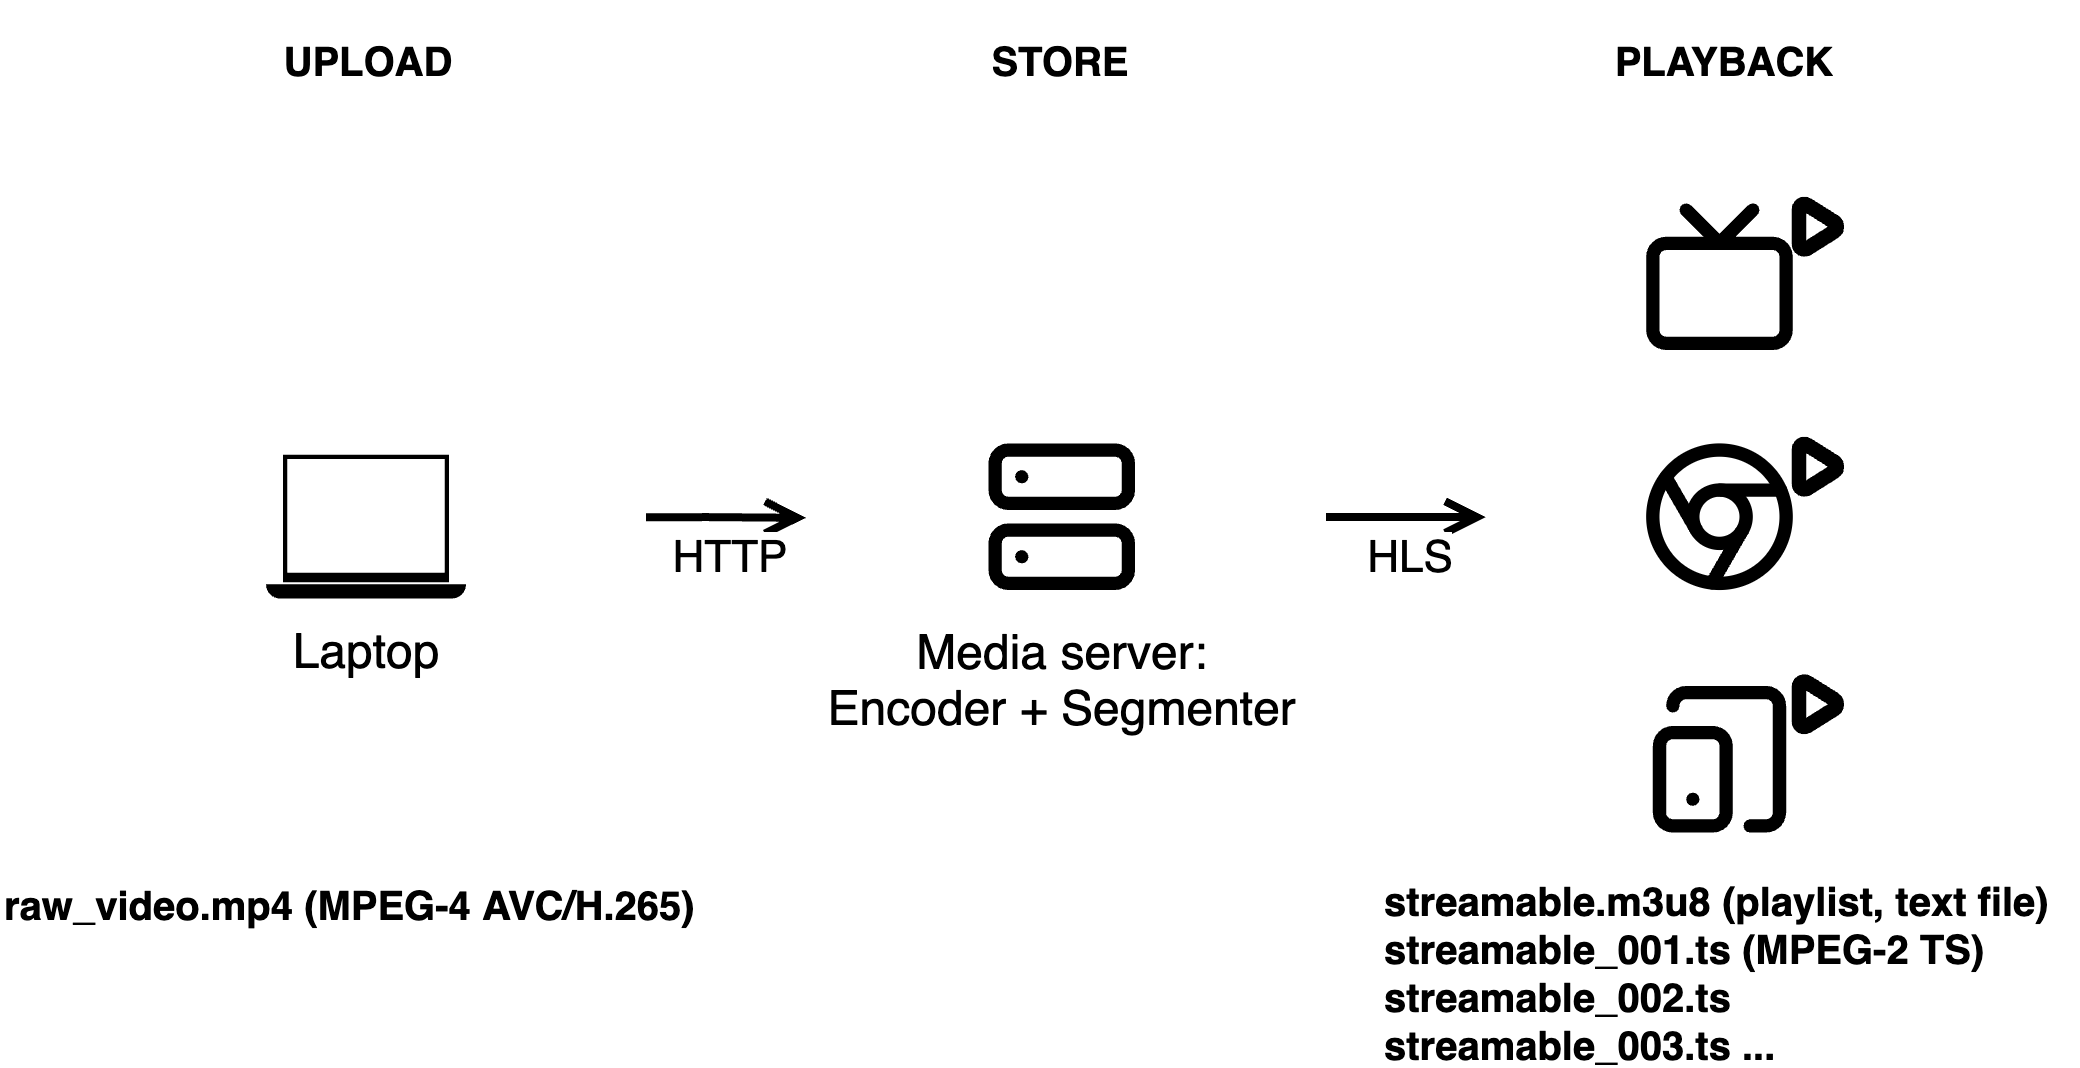
\includegraphics[width=120mm, keepaspectratio]{figures/dipterv_vodsetup.png}
	\caption{Példa egy VOD-kiszolgálás résztvevő eszközeire.}
	\label{fig:vodsetup}
\end{figure}

\begin{figure}[h]
	\centering
	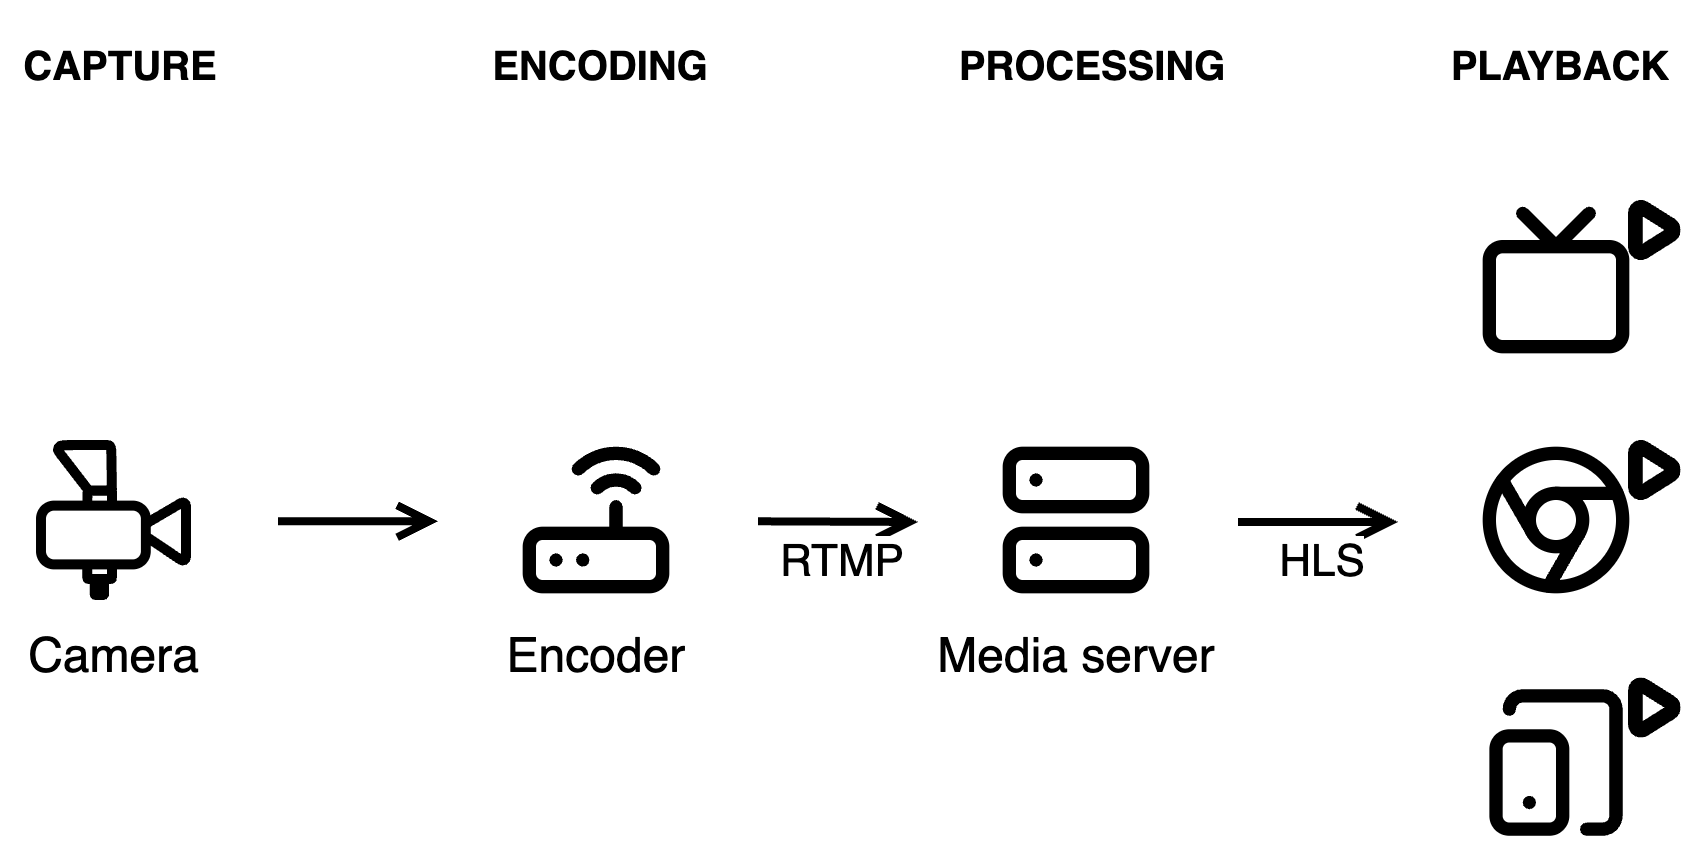
\includegraphics[width=90mm, keepaspectratio]{figures/dipterv_livesetup.png}
	\caption{Példa egy élő közvetítés résztvevő eszközeire.}
	\label{fig:livesetup}
\end{figure}

\subsection{Adaptive Bitrate Streaming}

A streamelést erősen befolyásoló tényező a hálózati feltételek változása, amelyek a videólejátszás minőségét és késleltetését is befolyásolják. Az \emph{Adaptive Bitrate Streaming} (ABR) egy a hálózati kiszolgálás során alkalmazott technika, amely megoldást jelenthet erre a problémára.

Az ABR során a forrásvideót több különböző bitrátával dolgozó kodekekkel és különböző felbontással kódoljuk a médiaszerveren, majd lejátszáskor a lejátszó alkalmazás a hálózati feltételek változására reagálva, valamint a fogadó fél számítási kapacitásától függően valós időben választja ki a megfelelő videó streamet ezek közül, onnan válogatja a packeteket (\refstruc{fig:ABR}).

\begin{figure}[h]
	\centering
	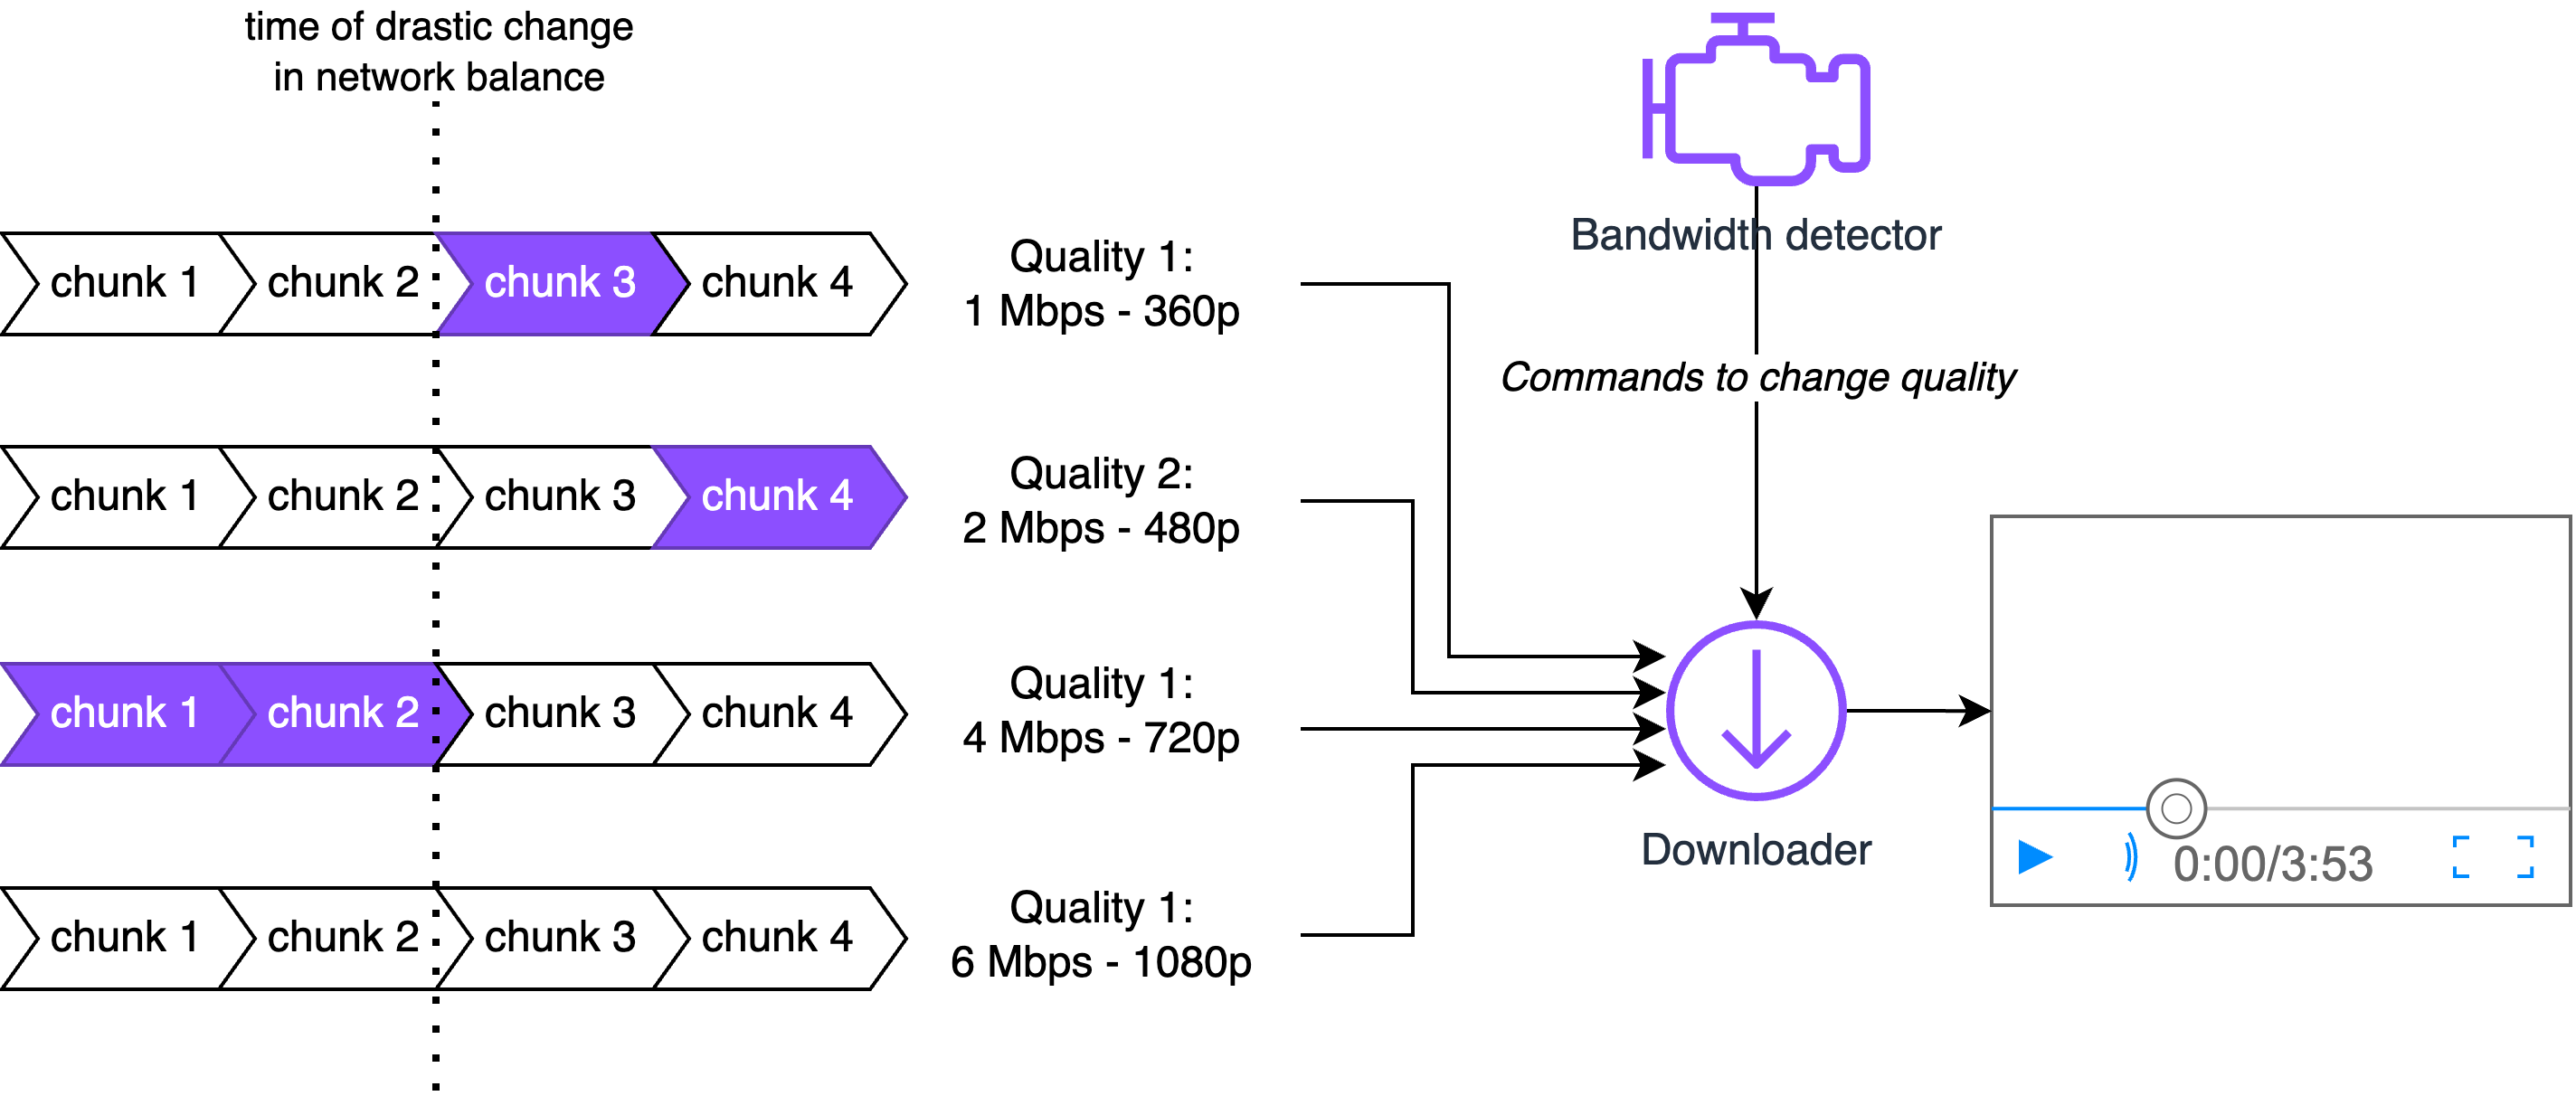
\includegraphics[width=140mm, keepaspectratio]{figures/dipterv_abr.png}
	\caption{Az Adaptive Bitrate Streaming működése.}
	\label{fig:ABR}
\end{figure}

Tiszta, hogy az ABR-t megvalósító rendszer előnyös mind a VOD, mind az élő közvetítés esetében, mivel a hálózati feltételek változása mindkét esetben előfordulhat. Az~automatikus stream váltogatás beavatkozás nélkül sokkal nagyobb \emph{Quality of Experience} (röviden QoE, magyarul az élmény minősége) lehetőségét tudja biztosítani\cite{DashAbr}. Az ABR-t alkalmazó rendszerek a videóadatokat több különböző bitrátával kódolják, ez természetesen a feldolgozási idejét a rendszereknek megnöveli, sőt élő közvetítés során egységnyi idő alatt jóval több számítási terhelést kell kibírnia a rendszernek.

\section{Videó streaming hálózati protokolljai}

Videó streamelésére -- másképp fogalmazva: valamely korábban ismertetett formátumban tárolt videófájl adatfolyamba való illesztésére -- különböző hálózati protokollok palettája áll rendelkezésünkre.

Néhány ismertebb célprotokoll létrejöttük időrendjében\cite{StreamingHistory}:

\begin{itemize}
	\setlength{\itemsep}{1pt}
  \setlength{\parskip}{0pt}
  \setlength{\parsep}{0pt}
	\item Real-Time Messaging Protocol (RTMP, 1996)
	\item Microsoft Smooth Streaming (MSS, 2008)
	\item Adobe's HTTP Dynamic Streaming (HDS, 2009)
	\item HTTP Live Streaming (HLS, 2009)
	\item WebRTC (2011)
	\item Dynamic Adaptive Streaming over HTTP (DASH, 2012)
\end{itemize}

A fent megnevezett alkalmazásrétegbeli protokollok (Layer 7) közül vizsgálják meg a~következő szekciók a négy legelterjedtebbet, kitérve arra is, milyen szállítási rétegű protokollokkal (Layer 4) tudnak együttműködni.

\subsection{Real-Time Messaging Protocol}

A Real-Time Messaging Protocolt (RTMP) nevű protokollt még a Macromedia nevű cég fejlesztette ki eredetileg. A vállalatot később az Adobe felvásárolta. Az RTMP egy teljes szervertől kliensig tartó protokoll, amely a Flash Player és a Flash Media Server közötti kommunikációra lett kifejlesztve eredendően. Közvetlen dolgozik a TCP felett, ennek nincs köze a~HTTP-hez.\cite{StreamingHistory} Az RTMP-t még támogatja sok-sok platform, mert egész alacsony késleltetést lehet vele elérni, egészen alacsony ``költségű''. A Twitch és a YouTube is támogatja, hogy RTMP pull üzemmódjában tudjunk ezeken a platformokon élő adást fogadni. Tehát szerveroldalon még használt, persze a Flash Player támogatásának 2020-as kivezetése miatt a protokoll használata kliensoldalon pedig visszaszorult.

\subsection{HTTP Live Streaming}

A HTTP-alapú streaming protokollok közül a legelterjedtebb a HTTP Live Streaming (HLS), amelyet az Apple fejlesztett ki 2009-ben. A HLS eredetileg az Apple jogvédett kereskedelmi protokolljaként indult, azóta viszont már szabad felhasználásúvá vált. Az~Apple`|eszközök -- macOS, iOS -- alapértelmezetten támogatják ezt a protokollt, és a modern böngészők is támogatják a \emph{Media Source Extensions} (MSE) API-n keresztül. A HLS a~HTTP felett dolgozik, egymástól független packetekre szedi a teljes kiszolgálandó videót, és az~RTMP-hez képest ez így állapotmentes adatforgalmazást tud megvalósítani.\cite{StreamingHistory}

HLS használata során H.264 formátumban kell a videóadatokat kódolni, a hangot AAC, MP3 vagy Dolby szabványokkal lehet kódolni. A konténerformátumot tekintve is kötött, MPEG-2 Transport Stream (MPEG-TS) formátumot használhatjuk, vagy pedig az MP4-et -- fMP4 technikával, azaz \emph{fragmented MP4-gyel}, ehhez pedig a Common Media Application Format (CMAF) konténerformátumra kell átalakítani.\cite{Cmaf} A darabokra szedést követően a packeteket egy lejátszási listában (.m3u8 kiterjesztésű szöveges indexfájl) tartja számon a szerver, amelyet a lejátszó alkalmazások letöltenek, és a lejátszás során a~megfelelő sorrendben és időzítéssel lejátsszák.\cite{HlsApple} Lásd a példát egy 720p-s streamet leíró indexfájlra \az+\ref{lst:m3u8example}. kódrészletben.

A HLS egy olyan protokoll, amely magában hordozza az ABR implementációját is, kliensoldalon modern Media Source Extensions funkcionalitást támogató böngészőkben elterjedt használni a \emph{hls.js}\footnote{\url{https://github.com/video-dev/hls.js}} nevű JavaScript-könyvtárat, amely implementálja a HLS protokollt. A .m3u8 indexfájl definiálhat több másik ilyen indexfájlt is, amelyek a különböző bitrátájú videóstreameket képviselik (pl. egy \emph{1080p.m3u8} fájl és egy \emph{720p.m3u8} fájl írja le a playlistjét egy-egy bitrátájú streamnek).

\begin{minipage}{0.92\textwidth}
	\begin{lstlisting}[
		caption=Részlet egy .m3u8 indexfájlból.,
		label=lst:m3u8example,
		style=tf,
    basicstyle=\fontsize{10}{12}\ttfamily,
	]
#EXTM3U
#EXT-X-VERSION:3
#EXT-X-TARGETDURATION:4
#EXT-X-MEDIA-SEQUENCE:1
#EXTINF:4.000000,
skate_phantom_flex_4k_2112_720p1.ts
#EXTINF:4.000000,
skate_phantom_flex_4k_2112_720p2.ts
#EXTINF:4.000000,
skate_phantom_flex_4k_2112_720p3.ts
#EXTINF:4.000000,
skate_phantom_flex_4k_2112_720p4.ts
#EXTINF:4.000000,
skate_phantom_flex_4k_2112_720p5.ts
\end{lstlisting}
\end{minipage}

\subsection{Dynamic Adaptive Streaming over HTTP}

A Dynamic Adaptive Streaming over HTTP -- röviden DASH vagy MPEG-DASH, tekintve, hogy a fejlesztője ennek is az MPEG csoport volt -- egy 2012-ben szabványosított protokoll. Hasonlít a HLS-hez, HTTP felett forgalmaz, sorozatba illeszt egymástól független packeteket. Ezeket a szegmentált packeteket egy \emph{manifest} fájlban tartja számon a~szerver (Media Presentation Description, MPD-fájl).\cite{Dash}

A HLS-hez képest ez a protokoll kodekagnosztikus, ami annyit jelent, hogy nem kötődik videókodekhez, használható H.264, H.265, akár VP9 is.\cite{DashIso} Igyekeztek ezzel a protokollal egyezményesíteni a tartalomvédelmet is, Common Encryptiont (CENC) használ titkosításra. Digitális jogkezelésre (Digital Rights Management, DRM) is agnosztikus. Amióta a HLS támogatja a CMAF konténerformátumban való szállítást, azóta könnyen át lehet arról állni akár DASH protokollra is, ugyanis a DASH is CMAF-alapú. A~DASH a~HTTP/2 protokollt is támogatja, sőt HTTP/3-at is már UDP felett.

A HLS-hez hasonló elvekkel dolgozik a DASH is, illetve ez is egy ABR technológiájú protokoll. A DASH implementációjára JavaScript-motorral rendelkező kliensekben -- böngészők, mobiltelefonok stb. -- a \emph{dash.js}\footnote{\url{https://dashjs.org/}} könyvtárat használják legtöbb esetben.

\subsection{WebRTC}

A WebRTC (Web Real Time Communications) egy nyílt forráskódú projekt részeként alapult -- támogatják kódbázisának fenntartását mind a Google, a Mozilla és az Opera csapatai is --, egy protokoll böngészőalapú valós idejű kommunikáció kialakítására. Ezt használja a Discord, a Google Chat és egyéb webes videóchat-alkalmazások.\cite{StreamingHistory}

A források és a streamet figyelők számának kardinalitása szempontjából ez eltér az előzőekben ismertetettektől -- amelyek egy forrás és több befogadóra optimalizáltak --, ez viszont peer-to-peer (P2P) alapú, tehát oda-vissza jellegű streamelést kell biztosítson. Emiatt a WebRTC a legjobb választás, amennyiben a felhasználási célja az, hogy a felhasználók közvetlenül egymással kommunikálhassanak, és nem szükséges közbeiktatni egy központi médiaszervert. Ezenkívül a WebRTC-t egyre szélesebb körben próbálják alkalmazni a~videó streaming területén is \emph{one-to-many} közvetítésre is. Szabad felhasználású kodekeket alkalmaz videó- és hangkódolás terén (pl.: Opus, VP9).\cite{WebRTC}

\chapter{Követelmények}

Egy nagyszabású, YouTube- vagy Netflix-szintű webes videó streaming szolgáltatás megvalósítása rendkívül összetett feladat, amely köré így kiterjedt technikai és üzleti követelményrendszert tudunk kialakítani. Egy ilyen rendszernek kezdetben biztosítania kell az~alapvető funkciókat, amelyet hétköznapi webalkalmazások is megvalósítanak, mint például a videók lejátszása során felmerülő interakciók kezelése. Azonban ahogy a platformunk népszerűsége növekedhet, újabb és újabb infrastrukturális igények merülhetnek fel: ezek teszik ki a nem funkcionális követelményeket, amik kiterjednek például a tartalomterjesztés minőségére, a biztonsági felkészültségére a webalkalmazásnak.

A következőkben részletezem azokat a követelményeket, elvárásokat, amelyeket szem előtt tartottam a streaming szolgáltatás megtervezésekor és megvalósításakor.

\section{Funkcionális követelmények}

A streaming szolgáltatást alapvetően egy központosított kliensoldali webes felületen keresztül lehet elérni, azon keresztül tudják adminisztrátorok kezelni a tartalmat. Ennek a~közvetlen frontoldali webes felületnek és a szolgáltatásainak a követelményeit érdemesnek tartottam csoportokba szedni:

\begin{itemize}
  \item Felhasználókezelésre vonatkozó funkciócsoport
        \begin{itemize}
          \item Habár a videók megtekintéséhez nincs szükség felhasználókezelésre és bejelentkezésre, viszont a videók kezeléséhez szükséges megvalósítani a felhasználók azonosítását és jogosultságkezelését.
          \item A felhasználók AuthSCH\footnote{\url{https://vik.wiki/AuthSCH}} segítségével tudnak bejelentkezni a rendszer ``stúdió'' nevezetű aloldalára, ahol a rendszer azonosítja őket AuthSCH-s profiljuk alapján, automatikusan jön létre felhasználói fiókjuk, regisztrációra külön nincs szükség.
          \item A felhasználók közötti különbséget a rendszerben adminisztrátorok és normál felhasználók között teszem meg, az előbbieknek jogosultságuk van a videók feltöltésére és kezelésére, az utóbbiaknak csupán bejelentkezésre későbbi adminisztrátorrá válásra, amennyiben másik adminisztrátor úgy dönt.
        \end{itemize}

  \item Videóprojektek kezelésére vonatkozó funkciócsoport
        \begin{itemize}
          \item Az adminisztrátorok a ``stúdió'' aloldalon tudnak új videóprojekteket létrehozni, amelyekhez a rendszer automatikusan generál egy egyedi azonosítót.
          \item Egy videóprojekt létrehozása után tudunk a videókhoz tartozó metaadatokat adni, azokon módosítani, mint például a cím, leírás, borítókép, kategória, résztvevő stábtagok.
          \item A videóprojektben lehetőség van egy darab MP4 konténerformátumú videó feltöltésére.
          \item Van lehetőség a videóprojekt teljes törlésére.
          \item A feltöltés után a felhasználói felület visszajelzést kell adjon arról, hol tart a~videó feltöltési folyamata, illetve a videókonvertálás folyamata a hálózati adatfolyamra való felkészítéshez.
          \item A ``stúdión'' kívüli oldalon a videóprojektek listázva vannak, ahol a nézők megtekinthetik a videóprojektek konkrét videóit stream formájában.
        \end{itemize}

  \item Élő közvetítés kezelésére vonatkozó funkciócsoport
        \begin{itemize}
          \item Az oldal kezdetlegesen csupán egy élő közvetítés adását támogatja, az adminisztrátor a ``stúdió'' aloldalon tudja ezt az egyetlen élő közvetítést indítani.
          \item A rendszer biztosítja, hogy fogadja egy külső forrásból (pl.: OBS Studio alkalmazásból) a felstreamelt videót a felhőn át és azt továbbítja a nézőknek.
          \item Az oldalon kell, legyen egy útvonal a nézők számára, ahol a közvetítés élőben megtekinthető.
        \end{itemize}
\end{itemize}

\section{Nem funkcionális követelmények}

A rendszerrel szemben támasztott nem funkcionális követelmények megállapításakor igyekeztem olyan dolgokra a hangsúlyt tenni, amelyek inkább számomra jelentenek kihívást, mivel nem terveztem a webalkalmazást úgy elkészíteni, hogy az valódi használatra készüljön -- azaz valódi haszna legyen és legyenek élő felhasználói a nagyvilágból, csupán a~kísérletnek volt része. Ezeket az elvárásokat a következőkben állapítottam meg:

\begin{itemize}
  \item Biztonság
  \begin{itemize}
    \item A megoldás kihasználja az AWS-felhő adta biztonsági lehetőségeket mind a hálózati struktúra kialakításakor, a webalkalmazás védelmezésére és a biztonságos kommunikáció (pl. HTTPS) kialakítására.
    \item A webalkalmazásban a felhasználók autentikációját és autorizációját a JWT`|tokenek segítségével oldom meg.
  \end{itemize}
  \item Hordozhatóság és könnyű karbantarthatóság
   \begin{itemize}
    \item Konténerizálom a szerveralkalmazást, hogy könnyen lehessen telepíteni és futtatni, egy egységként lehessen kezelni.
    \item A konténer és a buildelendő kódok automatikusan fordulnak és települnek a~CI/CD-folyamat részeként.
    \item A frissítések könnyedén kezelhetőek, erre alkalmazásra kerül konténerképeket tároló Docker Registry is.
    \item Eseményvezérelt architektúra az alkalmazás egyes folyamatainak megvalósítására és a szerveralkalmazás köré, hogy könnyen kiterjeszthető lehessen új funkcionalitásokkal.
    \item Az infrastruktúra kód formájában (Infrastructure as Code, IaC) is dokumentált, hogy könnyen lehessen újraépíteni a rendszert.
  \end{itemize}
  \item Elaszticitás
  \begin{itemize}
    \item Alkalmazásra kerül olyan futtatókörnyezet, amelyben könnyedén lehet az erőforrásokat növelni és csökkenteni, hogy a rendszer mindig a szükséges kapacitással rendelkezzen.
    \item Alkalmazásra kerül a CDN használata, hogy a videók gyorsan és megbízhatóan érhetőek legyenek el a nézők számára.
  \end{itemize}
  \item Költséghatékonyság
  \begin{itemize}
    \item Olyan szolgáltatások használata, amelyek csak a valóban szükséges erőforrásokat használják fel, és csak akkor, amikor azokra szükség van.
    \item A szolgáltatásokat úgy tervezem meg, hogy a lehető legolcsóbban lehessen őket üzemeltetni a kísérletezés során.
  \end{itemize}
\end{itemize}

\chapter{Felhasznált technológiák}

A fejezet célja, hogy bemutassa a videó streaming szolgáltatások implementációjához felhasznált konkrét szoftvereket, webes és felhőalapú szolgáltatásokat, valamint az azok közötti kapcsolatokat.

\section{FFMpeg szoftvercsomag}

Az FFMpeg\footnote{\url{https://www.ffmpeg.org/}} egy nyílt forráskódú és GPL-licenszelésű szoftvercsomag, amely képes videók és hangok kódolására, dekódolására, átalakítására (konvertálás), valamint streamelésre.\cite{ffmpeg} Az FFMpeg a legtöbb operációs rendszeren elérhető, videók és hangok kódolására és dekódolására szolgáló kodekeket tartalmaz, valamint számos különböző formátumot támogat, beleértve az MPEG-4, H.264, H.265, VP8, VP9, AV1, AAC, AC-3, Opus, és sok más formátumot. Folyamatosan frissen tartják a kodekeket, aktív fejlesztőbázissal rendelkezik.

A lokális videókonvertálásra és streamelésre az FFMpeg-csomagból az azonos nevű \verb|ffmpeg| parancssori interfészt (angolul Command-line interface, CLI) használtam. Beépítettem a webszerver-alkalmazásba egy külön szolgáltatásrészt, amely kihív a webszerver folyamatából és egy megfelelően felparaméterezett \verb|ffmpeg| parancsot futtat a videókonvertálásra és streamelés megkezdésére aszinkron módon, a kimeneti fájlokat a megfelelő helyre menti.

A felhőalapú megoldásban már nem került felhasználásra az FFMpeg, mivel az \emph{AWS Elemental} márkanév alatti szolgáltatásokat használtam a videókódolásra és streamelésre, viszont a szoftvercsomag közvetlen megismerése a videókonvertálás folyamatának megértését és a konvertálási folyamatok felparaméterezési lehetőségeinek mélyebb átlátását segítette.

\section{Open Broadcaster Software}

Az Open Broadcaster Software Studio (OBS Studio\footnote{\url{https://obsproject.com/}}) egy nyílt forráskódú, szabad szoftver, amelyet elsősorban élő közvetítésekhez és képernyőrögzítéshez használnak. Elterjedt Twitch-felhasználók körében. A program támogatja a Windows, macOS és Linux operációs rendszereket, és számos beállítási lehetőséget biztosít a felhasználók számára. Az OBS lehetővé teszi több videó- és hangforrás kombinálását, ennek köszönhetően webkamera felvétele, mikrofon inputja, az éppen használt képernyő képe vagy előre rögzített videók is kombinálhatóak a stúdió műszerfalán.

A szoftver kompatibilis a legnépszerűbb streaming platformokkal, így például You\-Tube-ra és Twitch-re is lehet feltölteni vele, és lehetőséget biztosít saját egyedi RTMP`|szerverekhez való csatlakozásra is rövid konfiguráció után. Az OBS Studio megbízható eszköz azok számára is, akik professzionális szintű élő közvetítést szeretnének megvalósítani.

\section{Amazon Web Services}

Az Amazon Web Services (AWS) a világ egyik legjobban elterjedt, legnagyobb szerverfarmjait fenntartó, vállalatok által is széles körben megbízható felhőszolgáltatója\cite{aws}. Felhasználói számára \emph{számítási, hálózati, adattárolási} célokat megvalósító szolgáltatások széles eszköztárát kínálja. Egyre feltörekvőbb az AWS az adattudomány területén is. Színes palettáját kínálja menedzselt szolgáltatásoknak mesterséges intelligencia megoldások összeillesztésére; valamint kiterjedt adatbázisok, adatfeldolgozó rendszerek építésére. Elsőként jut eszébe újonnan sokaknak az AWS, ha megbízható és könnyen skálázható webes szoftverrendszerek kialakítása a cél.

A felhasználók a szolgáltatásokhoz az AWS Management Console webes felületen keresztül, vagy az AWS Command Line Interface (AWS CLI) parancssori interfészén keresztül férhetnek hozzá. Az egyes felhasználók fel tudnak állítani maguknak egy vagy több AWS-fiókot, amelyek a számlázás és a jogosultságkezelés szempontjából elkülönülhetnek egymástól.

A fiókon belül lehetőséget kapunk granuláris jogosultságkezelésre, azaz az egyes felhasználók, szolgáltatások, vagy szolgáltatásrészek számára különböző alacsony szintű jogosultságokat adhatunk meg.

Az AWS regionális adatközpontokat üzemeltet a világ számos pontján, amelyek közül a felhasználók választhatnak, hogy melyik adatközpontban szeretnének szolgáltatásokat futtatni.

A költségeket ``pay-as-you-go'' alapelv alapján számolják fel, azaz a felhasználók csak az általuk használt szolgáltatások számítási kapacitásáért, a tárhelyért, az adatközpontból kifelé történő hálózati forgalomért fizetnek. A költségszámítási módszerek egyediek minden erőforrásra.

\subsection{AWS Elemental}\label{sec:aws_elemental}

Az Elemental Technologies 2006-ban indította vállalkozását streaming megoldások eladására. Egy jelentős mérföldkövük volt, amikor a szolgáltatásaikkal került közvetítésre a~2012. évi nyári olimpiai játékok Londonban. Az Elemental Technologies 2015-ben került az Amazon Web Services tulajdonába, azóta az AWS Elemental néven futó szolgáltatásokat kínálja az~AWS a felhőben. A fő célja a szolgáltatáscsomagnak, hogy óriási célközönségek számára is megbízható stream közvetítési megoldásokat kínáljon, amelyeket könnyen lehet skálázni, és amelyek a legújabb videókódolásokat és -technológiákat alkalmazzák.\cite{Elemental}

Szoftveres megoldásaik közül a legfontosabbak a következők:

\begin{itemize}
  \item \textbf{Elemental MediaConvert}: A MediaConvert egy felhőalapú videókódoló szolgáltatás, Software-as-a-Service (SaaS) jellegű, egy API-t ad, amelyen keresztül kódolási munkafolyamatokat (``jobokat'') indíthatunk. A MediaConvert támogatja a legnépszerűbb videóformátumokat, mint például a H.264, H.265, és a VP9, valamint a legújabb HDR (High Dynamic Range) és Dolby Vision technológiákat is. HLS streamre is képes felkészíteni a videókat. Csupán fel kell tölteni a forrásvideót egy S3-vödörbe, majd a konvertálás után a kimeneti videók számára is egy S3-vödröt tudunk megadni.
  \item \textbf{Elemental MediaLive}: Az Elemental MediaLive egy élővideó-kódoló szolgáltatás, amely lehetővé teszi a felhasználók számára, hogy élő adásokat fogadjanak és kódoljanak át a felhőben. A MediaLive támogatja élő videók legnépszerűbb feltöltési protokolljait, így az RTMP-t is. Ennek a használata már bonyolultabb, mint a~MediaConverté, nem szimplán csak egy API meghívásaként kell elképzelni. Külön csatornákat lehet benne definiálni, azokhoz inputot/inputokat rendelni, ezután pedig a kódolási munkafolyamatokat felkonfigurálni. Az AWS sokféle nyelvben garantál SDK-kat, amelyek segítségével könnyen lehet automatizáltan MediaLive-csatornákat indítani külön-külön adásokhoz.
  \item \textbf{Elemental MediaPackage}: Az Elemental MediaPackage készíti elő, csomagolja a~videófolyamot hálózati protokollokon szállítmányozásra, garantálja a biztonságos és folyamatos tartalomtovábbítást. Biztosíthatja VOD-ok S3-ból való tovább osztását, vagy élők tovább osztását a MediaLive-ból. A MediaPackage támogatja a~legnépszerűbb kliensfelőli protokollokat, ezek közé tartozik például a HLS, DASH és a Microsoft Smooth Streaming. Könnyedén integrálható CloudFront-disztribúciók originjaként.
\end{itemize}

Érdemes még a szoftveres megoldások közt megemlíteni az \emph{Elemental MediaConnectet}, amely egy Quality of Service (QoS) réteget biztosít a streamet fogadók és az AWS-felhő között, megbízható és biztonságos hálózati kapcsolatot biztosít. Ismert lehet még az \emph{Elemental MediaTailor}, amely lehetővé teszi a reklámok beillesztését a videófolyamainkba. Korábban még a felhozatalba tartozott, azonban kivezetésre kerül már az \emph{Elemental MediaStore} 2025. november 13-áig, amely egy objektumtároló szolgáltatás volt, viszont már az Amazon S3 kiváltotta, mivel az már erős \emph{read-after-write} konzisztenciát tud biztosítani 2020 óta.\cite{Mediastore}

Ezeken kívül az AWS szolgáltat még fizikai hardvereket is a streaming könnyítésére és a nagy számításigények kiszolgálására, ezek közé tartozik például a \emph{AWS Elemental Link}, amely egy HDMI- és SDI-portokkal rendelkező eszköz, lehetővé teszi a helyszíni videóforrások közvetlenül a felhőbe való továbbítását. A szoftveres és hardveres megoldások összekötésére egy példát szolgáltat mind VOD-ok és élő adások kiszolgálására \az+\refstruc{fig:vodlive}.

\begin{figure}
	\centering
	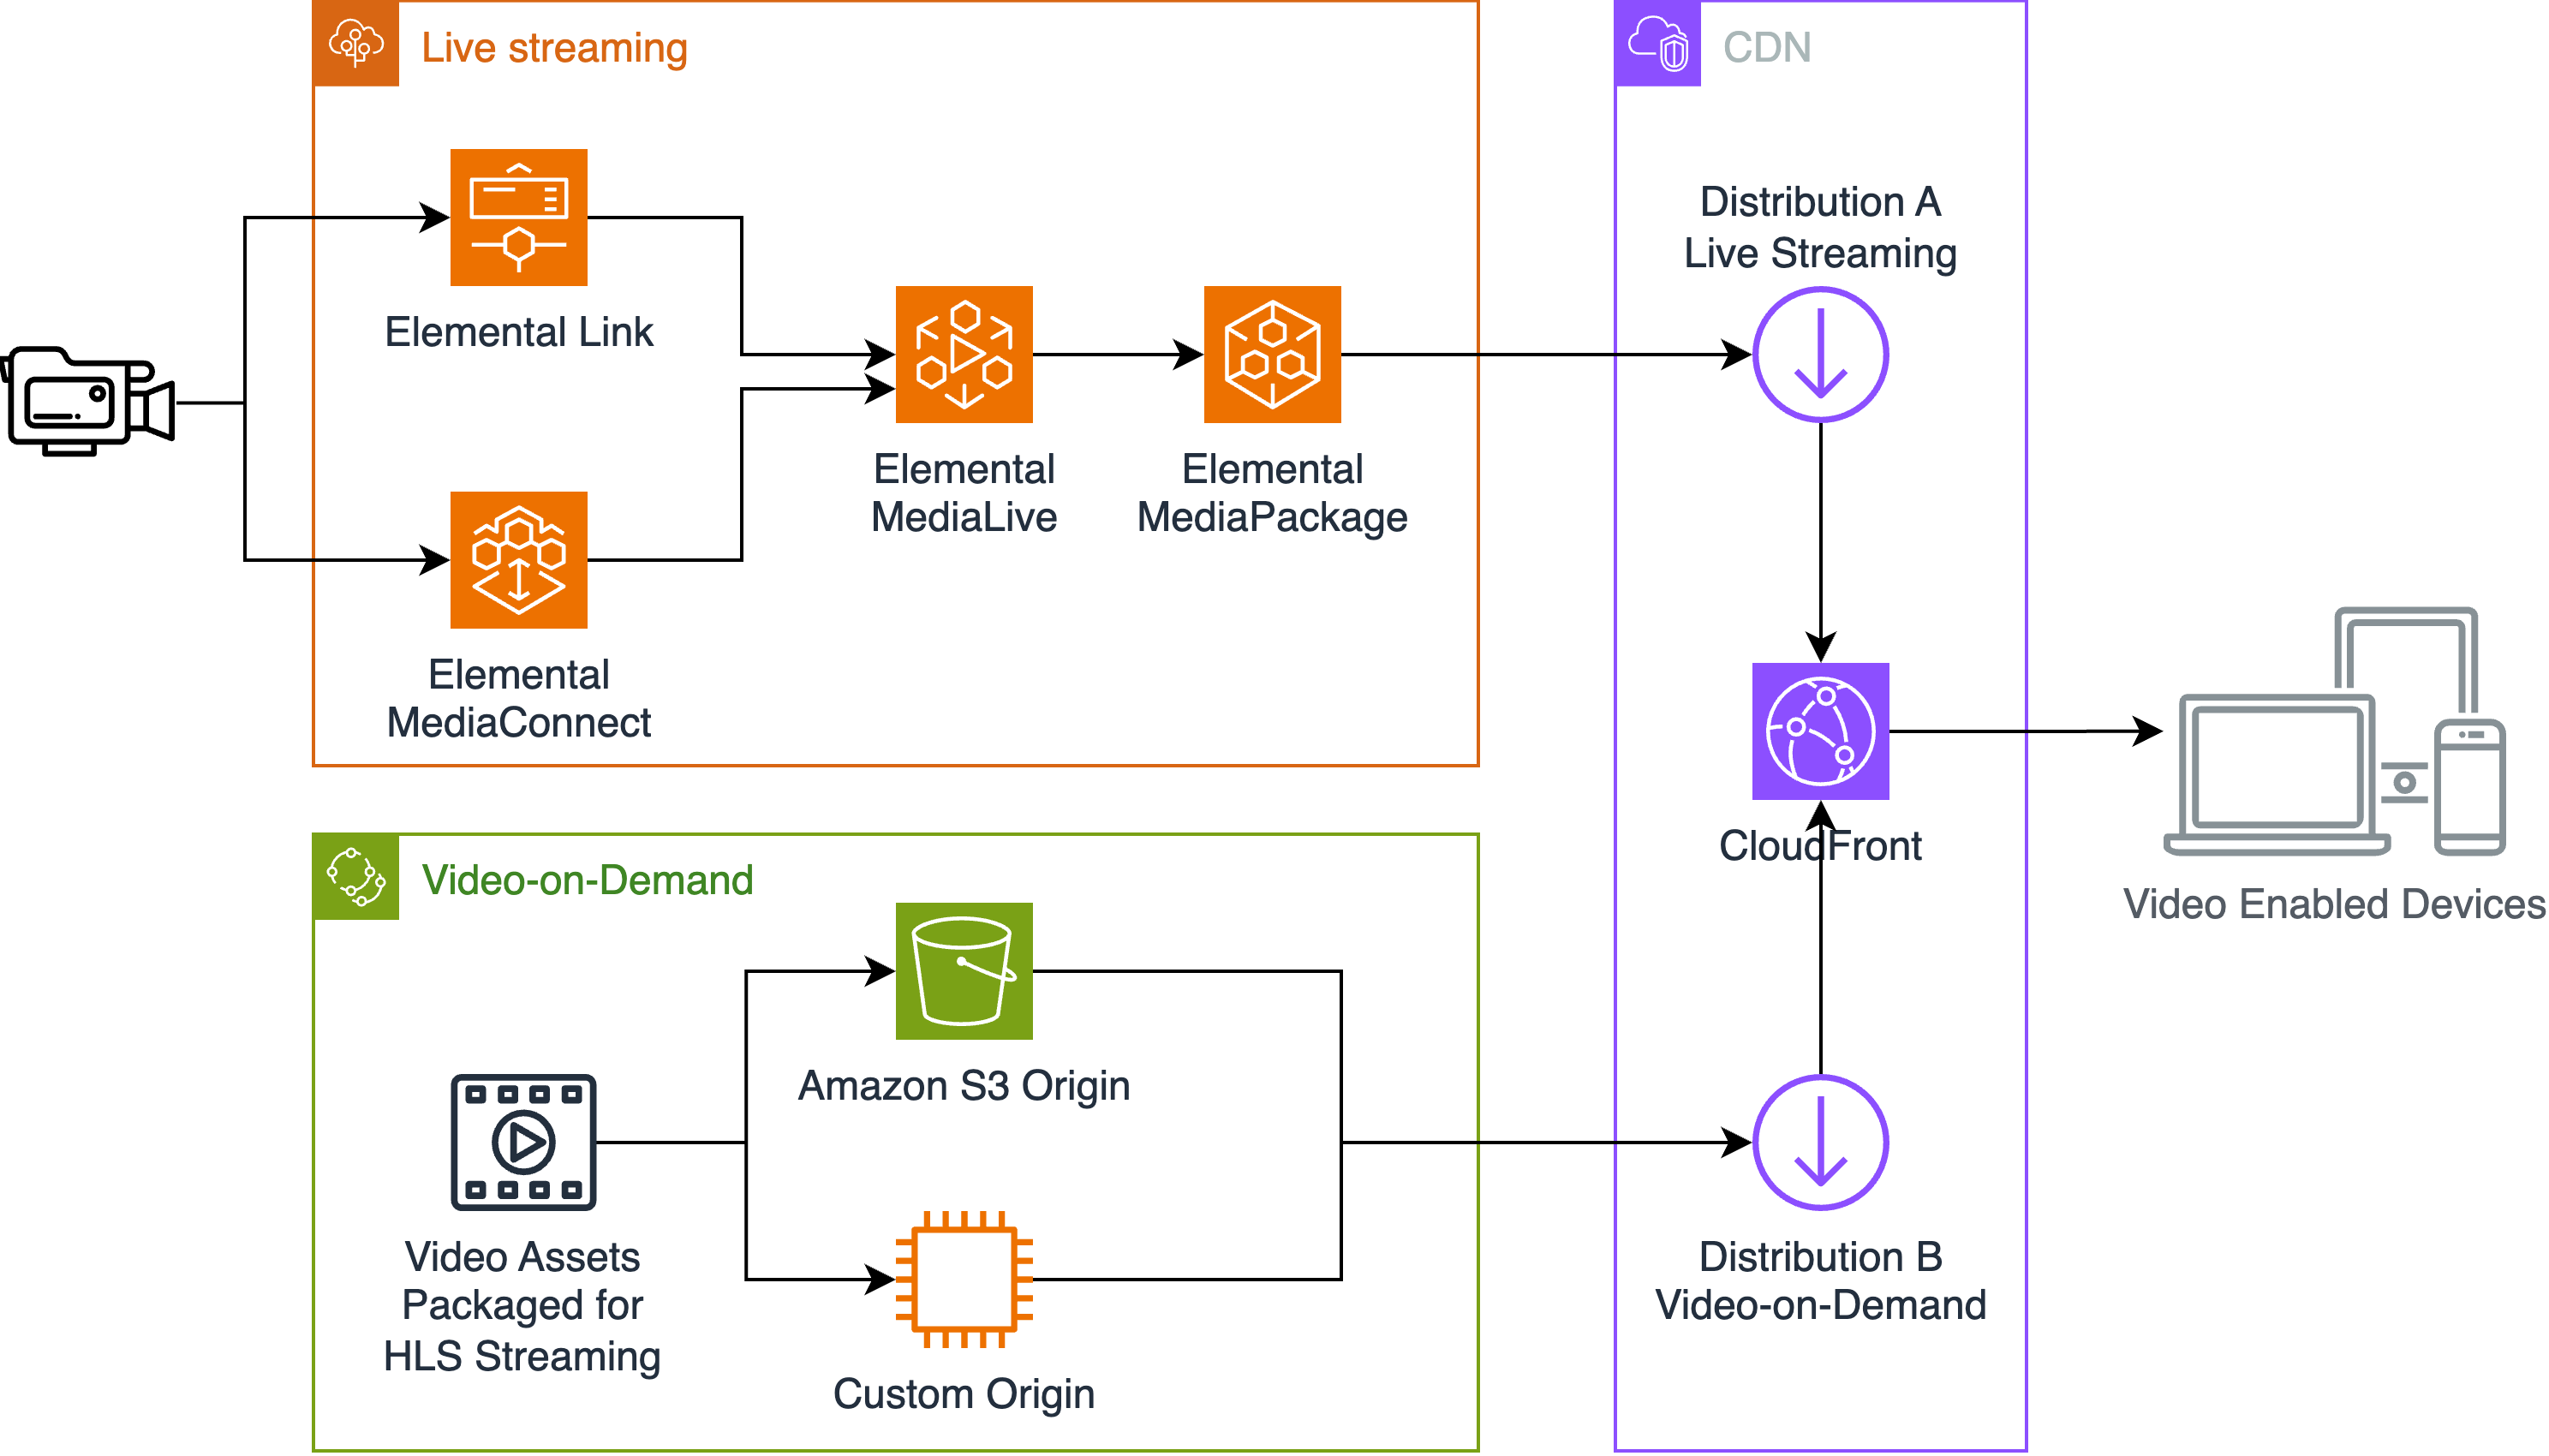
\includegraphics[width=150mm, keepaspectratio]{figures/dipterv_vodlive.png}
	\caption{Példa AWS Elemental szolgáltatások alkalmazására.}
	\label{fig:vodlive}
\end{figure}

\subsection{Amazon IVS}

Az Amazon Interactive Video Service (IVS) egy teljesen AWS menedzselte skálázható és megbízható élő videó streaming Software-as-a-Service, amely lehetővé teszi a fejlesztők számára, hogy gond nélkül integrálják az élő streaming funkcionalitását a saját alkalmazásaikba. Az IVS az~Elemental szolgáltatásokhoz képest end-to-end megoldást kínál kis késleltetésű többnézős alkalmazásra vagy garantált valós idejű alkalmazásra. Előbbi HLS-alapú kiszolgálást jelent körülbelül 5 másodperces késleltetéssel, utóbbi WebRTC-alapú kiszolgálást jelent.\cite{Ivs}

\begin{figure}[h]
	\centering
	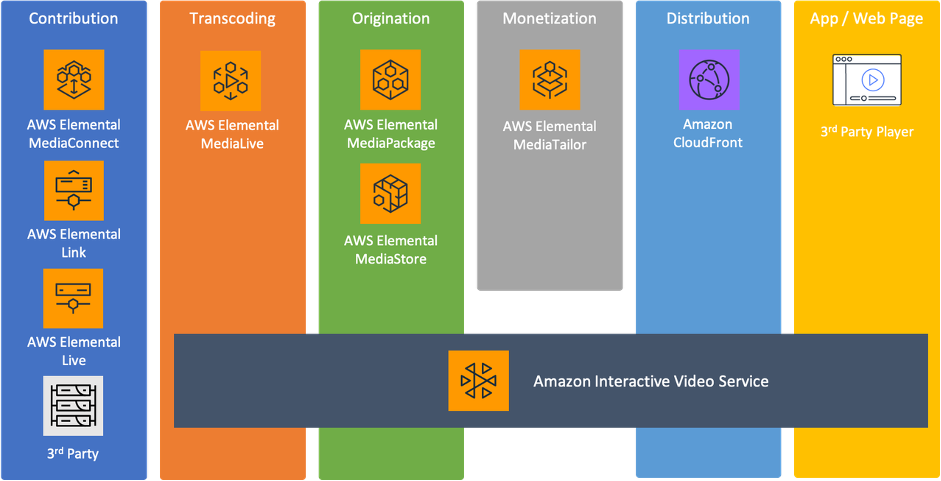
\includegraphics[width=150mm, keepaspectratio]{figures/aws_media.png}
	\caption{IVS és Elemental szolgáltatások összehasonlítása.}
	\label{fig:ivselemental}
\end{figure}

A forrásvideó-kódolástól a tartalomkiszolgálásig minden szükséges funkciót biztosít (\refstruc{fig:ivselemental}\footnote{A kép forrása: \url{https://aws.amazon.com/blogs/media/awse-choosing-aws-live-streaming-solution-for-use-case/}}), nekünk csupán a Software Development Kitjét (SDK) kell használni a saját alkalmazásunkban, és a többit az AWS-re bízhatjuk. Ezenkívül funkciókat biztosít chatszobák létrehozására és szavazások levezénylésére az adások keretében.

Ezen szolgáltatás ismertetése a megértést és a választás indoklását szolgálja későbbi fejezetekben, az Amazon IVS nem került felhasználásra a konkrét lefejlesztett rendszerben.

\subsection{AWS-szolgáltatások hálózatépítésre}

Az Amazon \emph{Virtual Private Cloud} (Amazon VPC) egy virtuális hálózati szolgáltatás. Vele megvalósítható, hogy az AWS publikus felhőjén belül is privát és publikus saját hálózatokat hozzunk létre. Az Amazon VPC segítségével a felhasználók teljes kontrollt gyakorolhatnak a virtuális hálózati környezetük felett, beleértve 

\begin{itemize}
	\setlength{\itemsep}{1pt}
  \setlength{\parskip}{0pt}
  \setlength{\parsep}{0pt}
	\item a VPC-k alatti alhálózatok IP-tartományainak konfigurálását,
	\item publikus IP-k lefoglalását,
	\item útvonaltáblák kitöltését,
	\item a hálózati interfészek/portok korlátozásait,
	\item egyéb hálózati eszközök -- NAT Gateway-ek, Internet Gateway-ek, valamint Transit Gateway-ek -- beillesztését,
	\item a hálózati teljesítmény felülvizsgálatát.
\end{itemize}

Különféle eszközöket kínál a felhasználók számára, hogy biztonságossá tegyék az AWS-felhőn belüli hálózati környezetüket. Priváttá tehetik alhálózataikat, bevezethetnek állapotmentes korlátozást ki- és bemenő forgalomra -- engedélyezett IP-tartományok és portok megadásával --, erre jók alhálózatokra alkalmazható \emph{Network Access Control Listek} (NACL), vagy a konkrét erőforrásokra alkalmazható \emph{Security Groupok}. Állapottartó és csomagellenőrzést végző megoldás az integrálható AWS Network Firewall. VPC Flow Logok bekötésével monitorozható válik a~hálózati forgalom is.

Az \emph{Application Load Balancer} (ALB) az Amazon Elastic Load Balancer (ELB) egy fajtája, ISO--OSI Layer 7 szinten, azaz alkalmazásrétegek szintjén működő terheléselosztó hálózati eszköz. Automatikusan skálázódik, lehetővé teszi a felhasználók számára, hogy egy vagy több szerver példány között egyenletesen eloszthassák a beérkező HTTP- és HTTPS`|kéréseket. Az ALB képes megkülönböztetni a kérések forgalmát például HTTP-fejléceik vagy URI-útvonalaik alapján.

\subsection{Amazon S3}

Az Amazon Simple Storage Service (Amazon S3) egy objektumtároló szolgáltatás, amely lehetővé teszi a felhasználók számára, hogy nagy mennyiségű adatot tároljanak az AWS`|felhőben ``vödrökben'' (bucketokban). Egy objektum egy fájl és azt a fájlt leíró metaadatok összessége. Egy vödör pedig objektumok tárolója.

\subsection{Amazon CloudFront}

Az előző fejezet egy szekciójában már említésre került a CDN mint a Video-on-Demand alapú streaming szolgáltatások egyik kulcsfontosságú eleme. Az Amazon CloudFront egy globális kiterjedésű CDN\cite{cdn}, amely lehetővé teszi a végfelhasználók számára, hogy a tartalmat hozzájuk közelebbi szervereken tárolt cache-ből töltsék le, ezáltal csökkentve a~késleltetést, csökkentve a~központi szerverek terhelését, és növelve a letöltési sebességet. Tartalmaink csoportosítására CloudFront-``disztribúciókat'' használunk.

A disztribúciók különböző URI-útvonalaikon akár különböző CDN-forrásokból -- úgynevezett ``originekből'' -- tudnak tartalmat kiszolgálni: ilyen origin lehet egy S3-vödör, AWS Elemental MediaPackage-alapú élő adást sugárzó csatorna, Amazon Application Load Balancer (ALB) példány, vagy akár egy egyéni HTTP-szerver is saját doménnévvel.

\subsection{Amazon ECS}

Az Amazon Elastic Container Service (ECS) arra szolgál, hogy konténeralapú alkalmazásokat, szoftvercsomagokat futtathassunk a felhőszolgáltatónál. Az ECS segítségével a~felhasználók könnyen futtathatnak és skálázhatnak konténereket anélkül, hogy a konténerek futtatásához szükséges infrastruktúra mélyén futó szervergépeket, valamint azok életciklusát, operációs rendszerének patch-elését kellene kezelniük -- ezek menedzselését az~AWS Fargate motor veszi át, mi csupán a környezeti paramétereket kell felkonfiguráljuk az igényeinknek megfelelően.

Ilyen paraméterek lehetnek: 

\begin{itemize}
	\setlength{\itemsep}{1pt}
  \setlength{\parskip}{0pt}
  \setlength{\parsep}{0pt}
	\item a konténerek képei,
	\item a konténerek alapvető számítási erőforrásai (CPU-magok száma, memória mérete),
	\item a konténerek hálózati beállításai (porttovábbítások, alkalmazott Security Group),
	\item a konténerek naplózása (hova továbbítódjanak a futtatás során a naplók),
	\item és a konténerek hozzáférési jogosultságai más AWS-szolgáltatásokhoz.
\end{itemize}

Tipikusan alkalmazott az ECS párban az Amazon \emph{Elastic Container Registry} (ECR) szolgáltatással, amely egy konténerképek tárolására szolgáló privát Docker Registry, amely lehetővé teszi a felhasználók számára, hogy a konténerek képeit biztonságosan tárolják és kezeljék az AWS-felhőben.

\subsection{Amazon RDS}

Az Amazon Relational Database Service (RDS) egy relációs adatbázis szolgáltatás, amely segít, hogy könnyen és hatékonyan hozhassunk létre, üzemeltessünk és skálázzunk relációs adatbázisokat az AWS-felhőben. Az RDS támogatja népszerű relációs adatbázisok motorjait, ezek közé tartozik a PostgreSQL, MySQL, MariaDB, Oracle Database és Microsoft SQL Server.

Képes automatikusan kezelni az adatbázisok frissítéseinek telepítését és a folyamatos biztonsági mentéseket. Mivel ezek is konkrét szervereket igényelnek, az RDS is könnyen integrálható az Amazon VPC hálózati környezetébe, a hálózati védelme is biztosítható.

\subsection{Kiegészítő AWS-szolgáltatások}

A konténerek orkesztrációjának kiegészítésére számos könnyen élesíthető és ECS-hez integrálható szolgáltatás áll rendelkezésre az AWS-felhőben, amelyek közül a legelterjedtebbek az Amazon CloudWatch Logs, az AWS Lambda és a Amazon EventBridge.

Az \emph{Amazon CloudWatch Logs} egy naplózó és monitorozó szolgáltatás, amely lehetővé teszi a felhasználók számára, hogy a konténerek futtatása során keletkező naplókat gyűjtsék, tárolják, és vizsgálják az ezekből származó metrikákat is akár.

Az \emph{AWS Lambda} egy serverless Function-as-a-Service (FaaS) szolgáltatás, amely lehetővé teszi kód függvényszerű futtatását anélkül, hogy szükség lenne a szerverek vagy a~futtatási környezet menedzselésére. A Lambda-függvény eseményekre reagálva kerül meghívásra, például HTTP-kérésekre, adatbázis-eseményekre, vagy más AWS-szolgáltatások eseményeire.

Ezzel kapcsolatban kerül a képbe az \emph{EventBridge}, az AWS központi eseménykezelő szolgáltatása, amely lehetővé teszi az egyes AWS-felhőszolgáltatásokon futó alrendszerek közötti kommunikációt. Segítségével szűrhetünk eseményekre, azokat könnyen továbbíthatjuk az egyes AWS-szolgáltatások között, a célpontja egy EventBridge által elkapott eseménynek ennek megfelelően egy Lambda-függvény is lehet.

\section{A webes komponensek technológiái}

A különböző felhőszolgáltatásokon futó kódbázisokat elterjedt webes technológiák segítségével fejlesztettem. Ezen technológiák kerülnek bemutatásra a következő szekciókban.

\subsection{TypeScript és JavaScript nyelvek}

A \emph{JavaScript} egy dinamikusan és gyengén típusos, interpretált programozási nyelv, amelyet webes alkalmazások fejlesztésére használnak. A böngészőben is JavaScript fut legtöbbször modern keretrendszerek (React.js, Vue.js vagy Angular) támogatásával a Document Object Model (DOM) renderelésére, manipulálására, ezzel tudjuk lehetővé tenni a kliensoldali webes alkalmazások interaktív működését, a felhasználói események kezelését, a HTTP`|kérések küldését.

Ezenkívül ez a nyelv használható szerveroldali környezetben is, az erre használatos \emph{Node.js} egy futtatókörnyezet, amely lehetővé teszi a JavaScript-kód futtatását a szerveroldalon is. A Node.js a V8 JavaScript-motorra épül, amely a Google Chrome böngészőben is fut, eseményvezérelt architektúrában szolgál ki függvényhívásokat, és aszinkron I/O`=működést biztosít, ami lehetővé teszi a blokkoló műveletek nélküli működést, maximalizálja a skálázhatóságot.\cite{Node}

A Node.js biztosítja különböző könyvtárakkal a HTTPS-alapú hálózati kommunikációt, a fájlrendszerműveleteket, a processzkezelést, a környezeti változók olvasását. A~funkcionalitások kiterjesztésére szokás használni JavaScript-modulokat, ekkor kerül középpontba az Node Package Manager (NPM) ökoszisztémája. Az NPM csomagkezelő segítségével könnyen telepíthetünk többek között Model-View-Controller alapú (MVC) keretrendszereket is (pl.: Express.js, NestJS), Object Relational Mapping (ORM) eszközöket (pl.: Prisma, TypeORM), SDK-kat (pl.: AWS SDK), vagy akár különböző adatbázis- és cache kezelőkhöz (pl.: PostgreSQL, Redis) drivereket a webszerverünk kiegészítésére.

A \emph{TypeScript} egy szuperhalmaza a JavaScriptnek -- azaz a JavaScript szintaxisát bővíti ki --, amely szigorú és statikus típusosságot ad hozzá. Bármely a nyelven írt kód a TypeScript`|fordító (\emph{tsc} -- TypeScript Compiler, CLI-alapú eszköz) segítségével JavaScript-kóddá alakítható. A TypeScript segítségével a fejlesztők könnyebben tudják a kódjukat karbantartani, mivel a típusok segítenek a hibák felismerésében, statikus analízisben, és a kódolás során a fejlesztőknek segítségére lehet a kód kiegészítésében is. Kliens- és szerveroldalon is használatos, a Node.js natívan nem támogatja, de vannak futtatókörnyezetek, amelyek fordítás nélkül is már támogatják a TypeScript futtatását (pl.: Deno).

A TypeScript-alapú technológiákból felépülő ``stackek'' előnye, hogy a kliens- és szerveroldali kódokat ugyanabban a nyelvben írhatjuk meg, így a fejlesztőknek nem kell külön-külön nyelveket és környezeteket tanulniuk, valamint a kódok könnyebben átírhatók, újrahasznosíthatók és könnyebben karbantarthatók.

Mellékesen érdemes még megemlíteni, hogy az AWS CloudFront szolgáltatása lehetőséget nyújt a felhasználóhoz közel futó edge szerverfarmokon nagyon kicsi számításigényű függvényeket futtatni, amelyeket a felhasználói kérésekre lehet közvetlen ráereszteni. Ezeknek két típusa is létezik: a CloudFront Function-függvények felprogramozása egy korlátozottabb nyelvi lehetőségekkel rendelkező JavaScriptben történik, míg a Lambda@Edge`|függvények logikája lehet Node.js futtatókörnyezet feletti JavaScriptben, illetve akár Python nyelven megírva.

\subsection{React}

A React\footnote{\url{https://react.dev/}} egy nyílt forráskódú JavaScript-könyvtár, amelyet a Facebook (ma Meta) fejlesztette ki még akkoriban belső fejlesztőeszközként. Single Page Applicationök (SPA) fejlesztésére használt. A React a komponensalapú fejlesztést támogatja, amivel úgy tudunk építkezni, hogy az felhasználói felületet (angolul \emph{User Interface}, röviden UI) kisebb, újrahasznosítható építőelemekre bontjuk. Az egyik fő előnye a \emph{virtuális DOM} fenntartása, amely hatékonyan kezeli a változásokat és javítja a teljesítményt.

A React alapvetően \emph{kliensoldali renderelést} (angolul Client-Side Rendering, CSR) használ, ami azt jelenti, hogy az alkalmazás a böngészőben fut, és a szerver csak egy alapszintű HTML-t küld, hozzá a JavaScriptet. Azonban nagyobb alkalmazásoknál gyakran szükség van más renderelési módszerekre: \emph{Server-Side Rendering} (SSR) esetén a React-alkalmazás HTML-jét a szerver generálja le és küldi el a böngészőnek. Ez javítja a teljesítményt és a~keresőoptimalizálást (angolul Search Engine Optimization, SEO), mert a keresőmotorok számára az oldal már előre renderelve érkezik. Egy másik ilyen módszer a \emph{Static Site Generation} (SSG), amely során az oldalak statikusan generálódnak a buildelési folyamat során. Ez gyors betöltési időt eredményez. A \emph{Next.js}\footnote{\url{https://nextjs.org/}} egy React köré épített keretrendszer, amely mind SSG- és SSR-funkcióval is rendelkezik.

Gyakori, hogy webes keretrendszer nélkül csupán statikus weboldalakat generálunk React felhasználásával. A \emph{Vite} egy olyan buildelési eszköz, amely gyorsítja a fejlesztési folyamatot, és képes React alkalmazásával írt -- vagy épp más egyéb, például Vue.js-ben írt -- TypeScript- vagy JavaScript`|projekteket is statikus weboldalakká generálni.

A React egy nagyon népszerű keretrendszer, amelyet a fejlesztők széles körben használnak, és amelynek számos kiegészítő könyvtára és eszköze van, amelyek segítségével gyorsan és hatékonyan lehet webes felületeket fejleszteni. Ennek megfelelően széleskörben támogatott és szeretett könyvtárakat lehet beépíteni a React-alapú alkalmazásokba, mint például

\begin{itemize}
	\setlength{\itemsep}{1pt}
  \setlength{\parskip}{0pt}
  \setlength{\parsep}{0pt}
	\item a React Router, SPA-n belüli routingra,
	\item a TanStack Query, egyszerűsített állapotkezelő aszinkron kérésekre,
	\item a React Hook Forms, gyors és hatékony formkezelésre.
\end{itemize}

\section{Üzemeltetési technológiák}

Végül pedig a fejlesztés során használt üzemeltetési technológiákat ismertetem, amelyek segítik a karbantarthatóságot, illetve amelyek segítségével a fejlesztők könnyen tudják a~kódbázisból az alkalmazásokat futtatni, az infrastruktúrát felhúzni.

\subsection{Docker}

A virtualizáció egy típusa a \emph{konténerizáció}, amely lehetővé teszi a fejlesztők számára, hogy az alkalmazásokat virtuális gépeknél egyszerűbb ``konténerekbe'' csomagolják, abból képet generáljanak, azt pedig könnyen osszák tovább, és ezekből a képekből konténereket futtathassanak a számítógépükön vagy épp a felhőben. Egy virtuális gép a gazdagép hardvereit virtualizálja, a konténer pedig a gazda operációs rendszert virtualizálja, azaz a konténerek alatt közös a \emph{kernel} (\refstruc{fig:virtudocker}\footnote{A kép forrása: \url{https://www.atlassian.com/microservices/cloud-computing/containers-vs-vms}}). Ezzel elveszik a teljes izoláció, azaz a biztonság, de a konténerek könnyebbek, gyorsabban indulnak -- hisz nincs \emph{bootolási idő} --, és kevesebb erőforrást használnak. 

\begin{figure}[h]
	\centering
	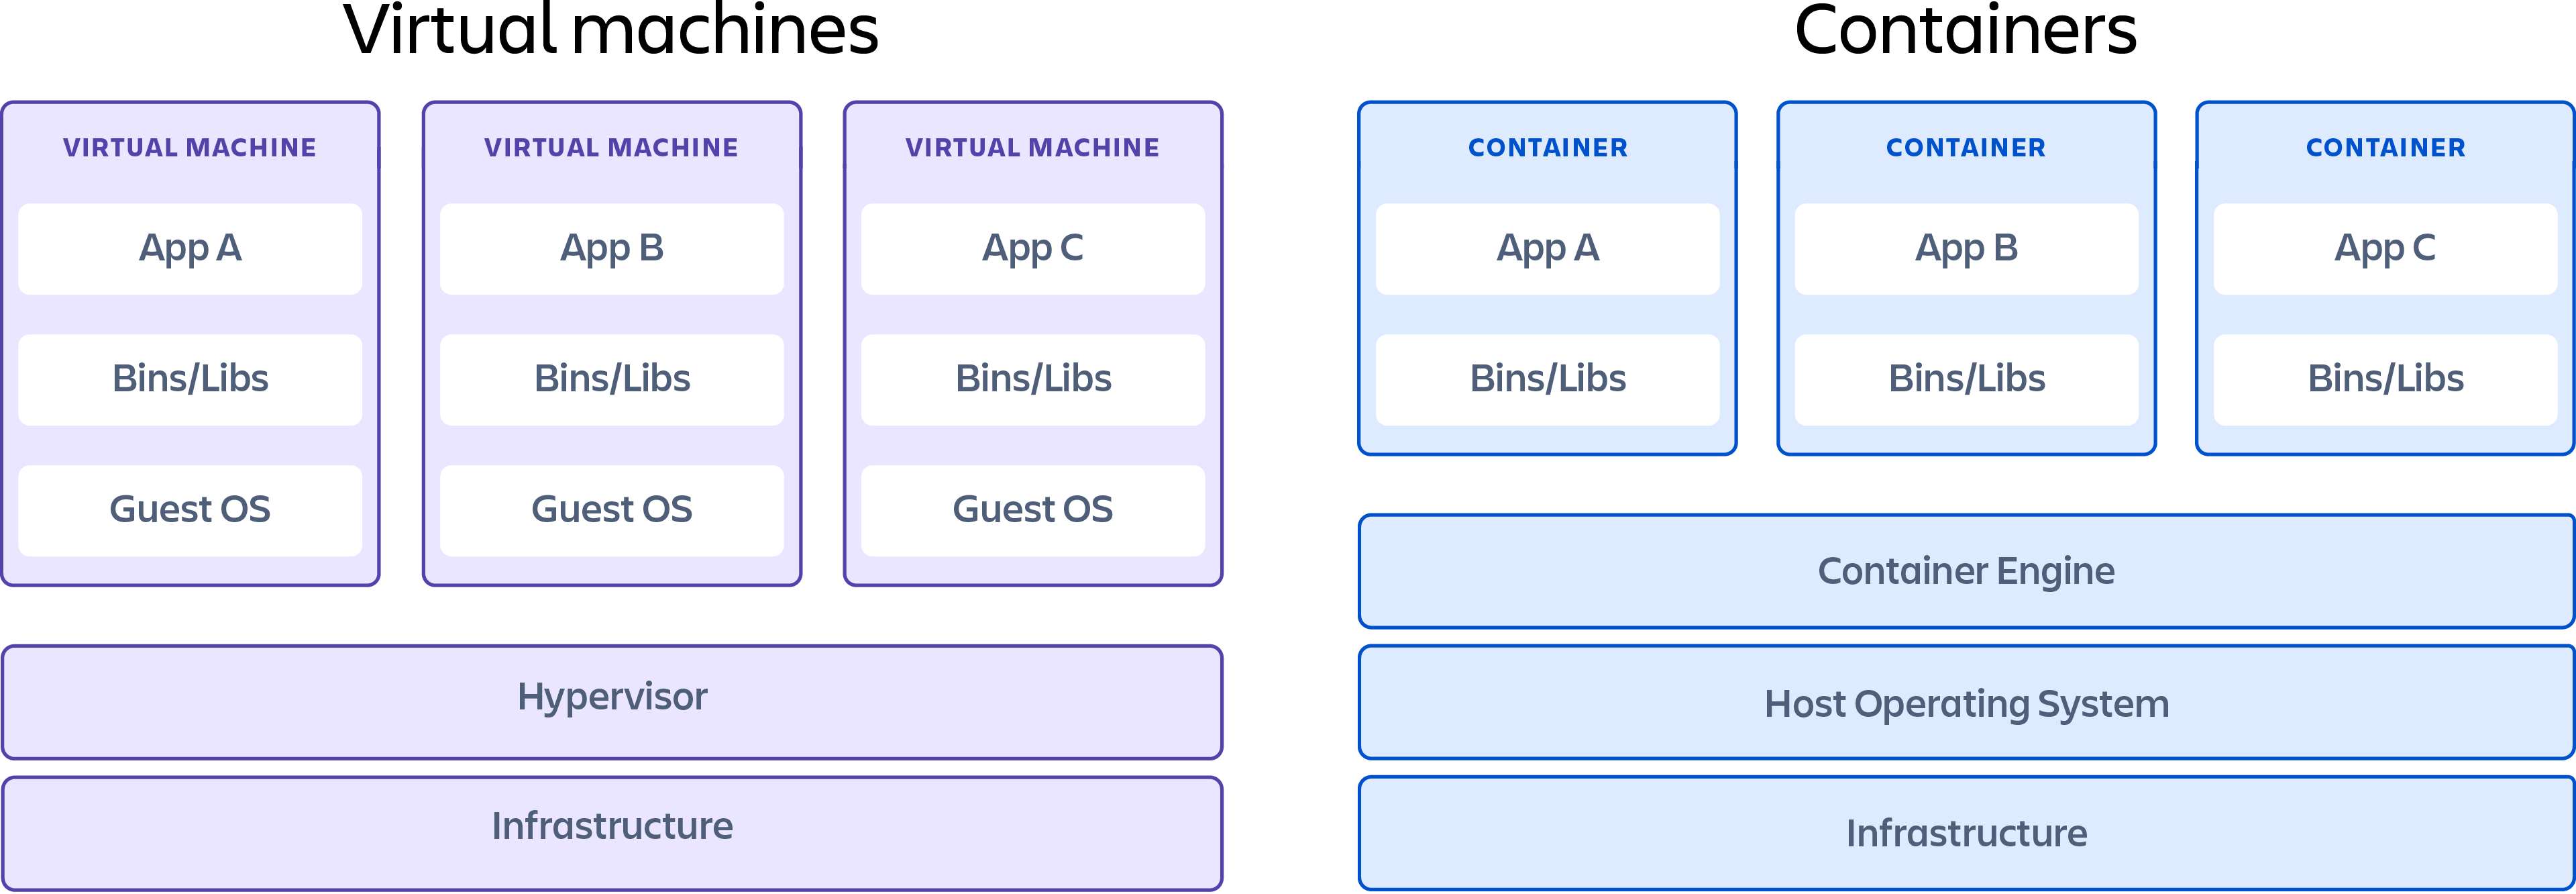
\includegraphics[width=120mm, keepaspectratio]{figures/virtudocker.png}
	\caption{Virtuális gépek és konténerek összehasonlítása.}
	\label{fig:virtudocker}
\end{figure}

A konténer egyfajta szabványosított egység, amely tartalmazza az alkalmazás kódját, a szükséges függőségeket (könyvtárakat), a konfigurációs fájlokat, és amire az alkalmazásnak szüksége van a futtatáshoz.

A \emph{Docker} egy konténerizációs fejlesztői környezet, a mélyén a \emph{containerd} névre keresztelt motor fut konténerizációs futtatókörnyezetként.\cite{Docker} Lehetővé teszi a konténerek létrehozását, indítását, kezelését és átvitelét. Virtuális tárhelyet és hálózatot biztosít a~konténerek számára, és lehetővé teszi a konténerek közötti biztonságos kommunikációt. A~Docker egy nyílt forráskódú projekt, amelyet a fejlesztők széles körben használnak a~konténerizált alkalmazások fejlesztésére és futtatására.

\subsection{GitHub}

Szoftverrendszerek, alkalmazások fejlesztése során szinte elengedhetetlen a verziókezelés, amelynek segítségével a fejlesztők nyomon követhetik a kódbázis változásait, visszaállíthatják az előző verziókat, és könnyen együtt tudnak dolgozni a kódon. Erre a munkafolyamatra az egyik legelterjedtebb \emph{Source Code Management} (SCM) eszköz a Git verziókezelő. A Git egy elosztott verziókezelő rendszer. Minden fejlesztő saját gépén tárolja a teljes kódbázisát, majd a módosításokat a felhőben lévő tárolóval szinkronizálhatja.

A Git szoftver köré széleskörben találhatunk felhőtárhely-szolgáltatókat, ezek közül a legnépszerűbb a GitHub\footnote{\url{https://github.com/about}}. A GitHub a tárhelyen kívül sok más funkcionalitást is szolgáltat a hatékony együttműködés és kódgondozás kivitelezésére, egy ilyen szolgáltatása a GitHub Actions, amely CI/CD-folyamatok kezelésére egy eszköz, olyan folyamatokra hasznosítható, mint a statikus ellenőrzés, a build folyamatok automatizálása, és például a~kód AWS-re való kiélesítése is.

\subsection{Terraform}

A Terraform\footnote{\url{https://www.terraform.io/}} egy elterjedt \emph{Infrastructure as Code} (IaC) eszköz, amely lehetővé teszi a~felhasználók számára, hogy infrastruktúrát definiáljanak kódban, és ezt az infrastruktúrát automatizáltan hozzák létre, módosítsák és töröljék. A Terraform a felhőszolgáltatók API-jait, illetve Cloud Development Kitjét (CDK) használja az változtatások érvényre juttatására. Go nyelven íródott a motorja, a Terraform IaC-ra pedig a saját HashiCorp Configuration Language (HCL) nyelvét ajánlja, amely egy deklaratív nyelv.

\chapter{A tervezett architektúra}

A következőkben részletezem a tervezett architektúrát két nézetben: első körben az architektúra logikai felépítését mutatom be, majd a konkrét fizikai felépítését az AWS-felhőben. A logikai felépítés a követelmények alapján készül függetlenül egy választott platformtól, tükrözi az alapszintű kommunikációs modelljét a rendszernek, bemutatja a magas szintű összetartozó rendszeregységeket, amikre lehet bontani a teljes egészet. Segít a megrendelőnek -- aki nem feltétlen teljesen tapasztalt a területen -- megérteni a mérnöki terveket. A~fizikai felépítés konkrét önállóan felprogramozható és konfigurálható szoftverkomponenseket integrál a tervrajzba. Elsősorban a fejlesztőknek szól, akik a rendszer megvalósításáért felelősek.

\section{Logikai felépítés}

A logikai felépítést legjobban \az+\refstruc{fig:highlevel} tudja jól bemutatni. A rendszer három fő komponenscsoportra bontható a követelmények alapján: a kliensközeli csoportra, a szerveroldali csoportra és az ``orkesztrációs'' csoportra. A kliensközeli csoport szolgálja ki a felhasználókat tartalommal, a szerveroldali csoport kezeli az hagyományos üzleti logikát, ahogy az egy többrétegű webalkalmazás megvalósításánál is megszokott az iparban. Az utolsó csoportot ``orkesztrációs'' csoportnak neveztem el, mivel ez szereli fel a két csoportot tartalommal, kezeli események hatására a videófeldolgozást a háttérben.

Érdekes lehet megfigyelni, hogy az egyes csoportok konkrét megvalósítása akár kicserélhetővé válik, egy-egy csoport mögötti teljes szoftvercsomag könnyen lekapcsolható a~másik kettőről, csupán jól definiált és agnosztikus API-okra van szükség.

A kliensközeli csoportban a felhasználók a webalkalmazást saját kliensükre egy erre szolgáló tárolóból kell letöltsék, hasonlóképp érik el a videókat két tárolóból. Ezzel a funkcionális követelmények megvalósulnak az élők elérésére, a VOD-ok elérésére, a weboldalon a videóprojektek UI-jára vonatkozó követelmények. A nem funkcionális követelményekből pedig teljesül a caching komponenssel, hogy a videók gyorsan és megbízhatóan érhetőek el a nézők számára.

A szerveroldali csoportban darabokra szedve tulajdonképpen egy REST API helyezkedik el élő adást kezelő, VOD-kezelő és felhasználókezelő komponensekkel közösen. Ez API-átjáró mögé van helyezve, amely a biztonságos kommunikációt tudja biztosítani, a~felhasználók autentikációját és autorizációját tudja kezelni együttműködve a felhasználókezelő komponenssel, valamint a kliensnek a megfelelő interakciós lehetőséget tud szolgáltatni. A szerveroldali csoportban a videók feltöltése történik csupán, az egyes entitásokról a~változások nyilvántartása kerül még tárolásra.

A szerveroldali csoport események formájában kommunikál az élőadás- és VOD-kezelő az ``orkesztrációs'' csoportban lévő eseménykezelővel. Az orkesztrációs réteg fogja a két csoportot össze, események hatására indíttat konvertálást a konvertáló komponenssel. Ez a komponens tölti fel a videókat a kliensközeli csoport felé, tart összeköttetést a live streaming külső forrásával.

\begin{figure}[h]
	\centering
	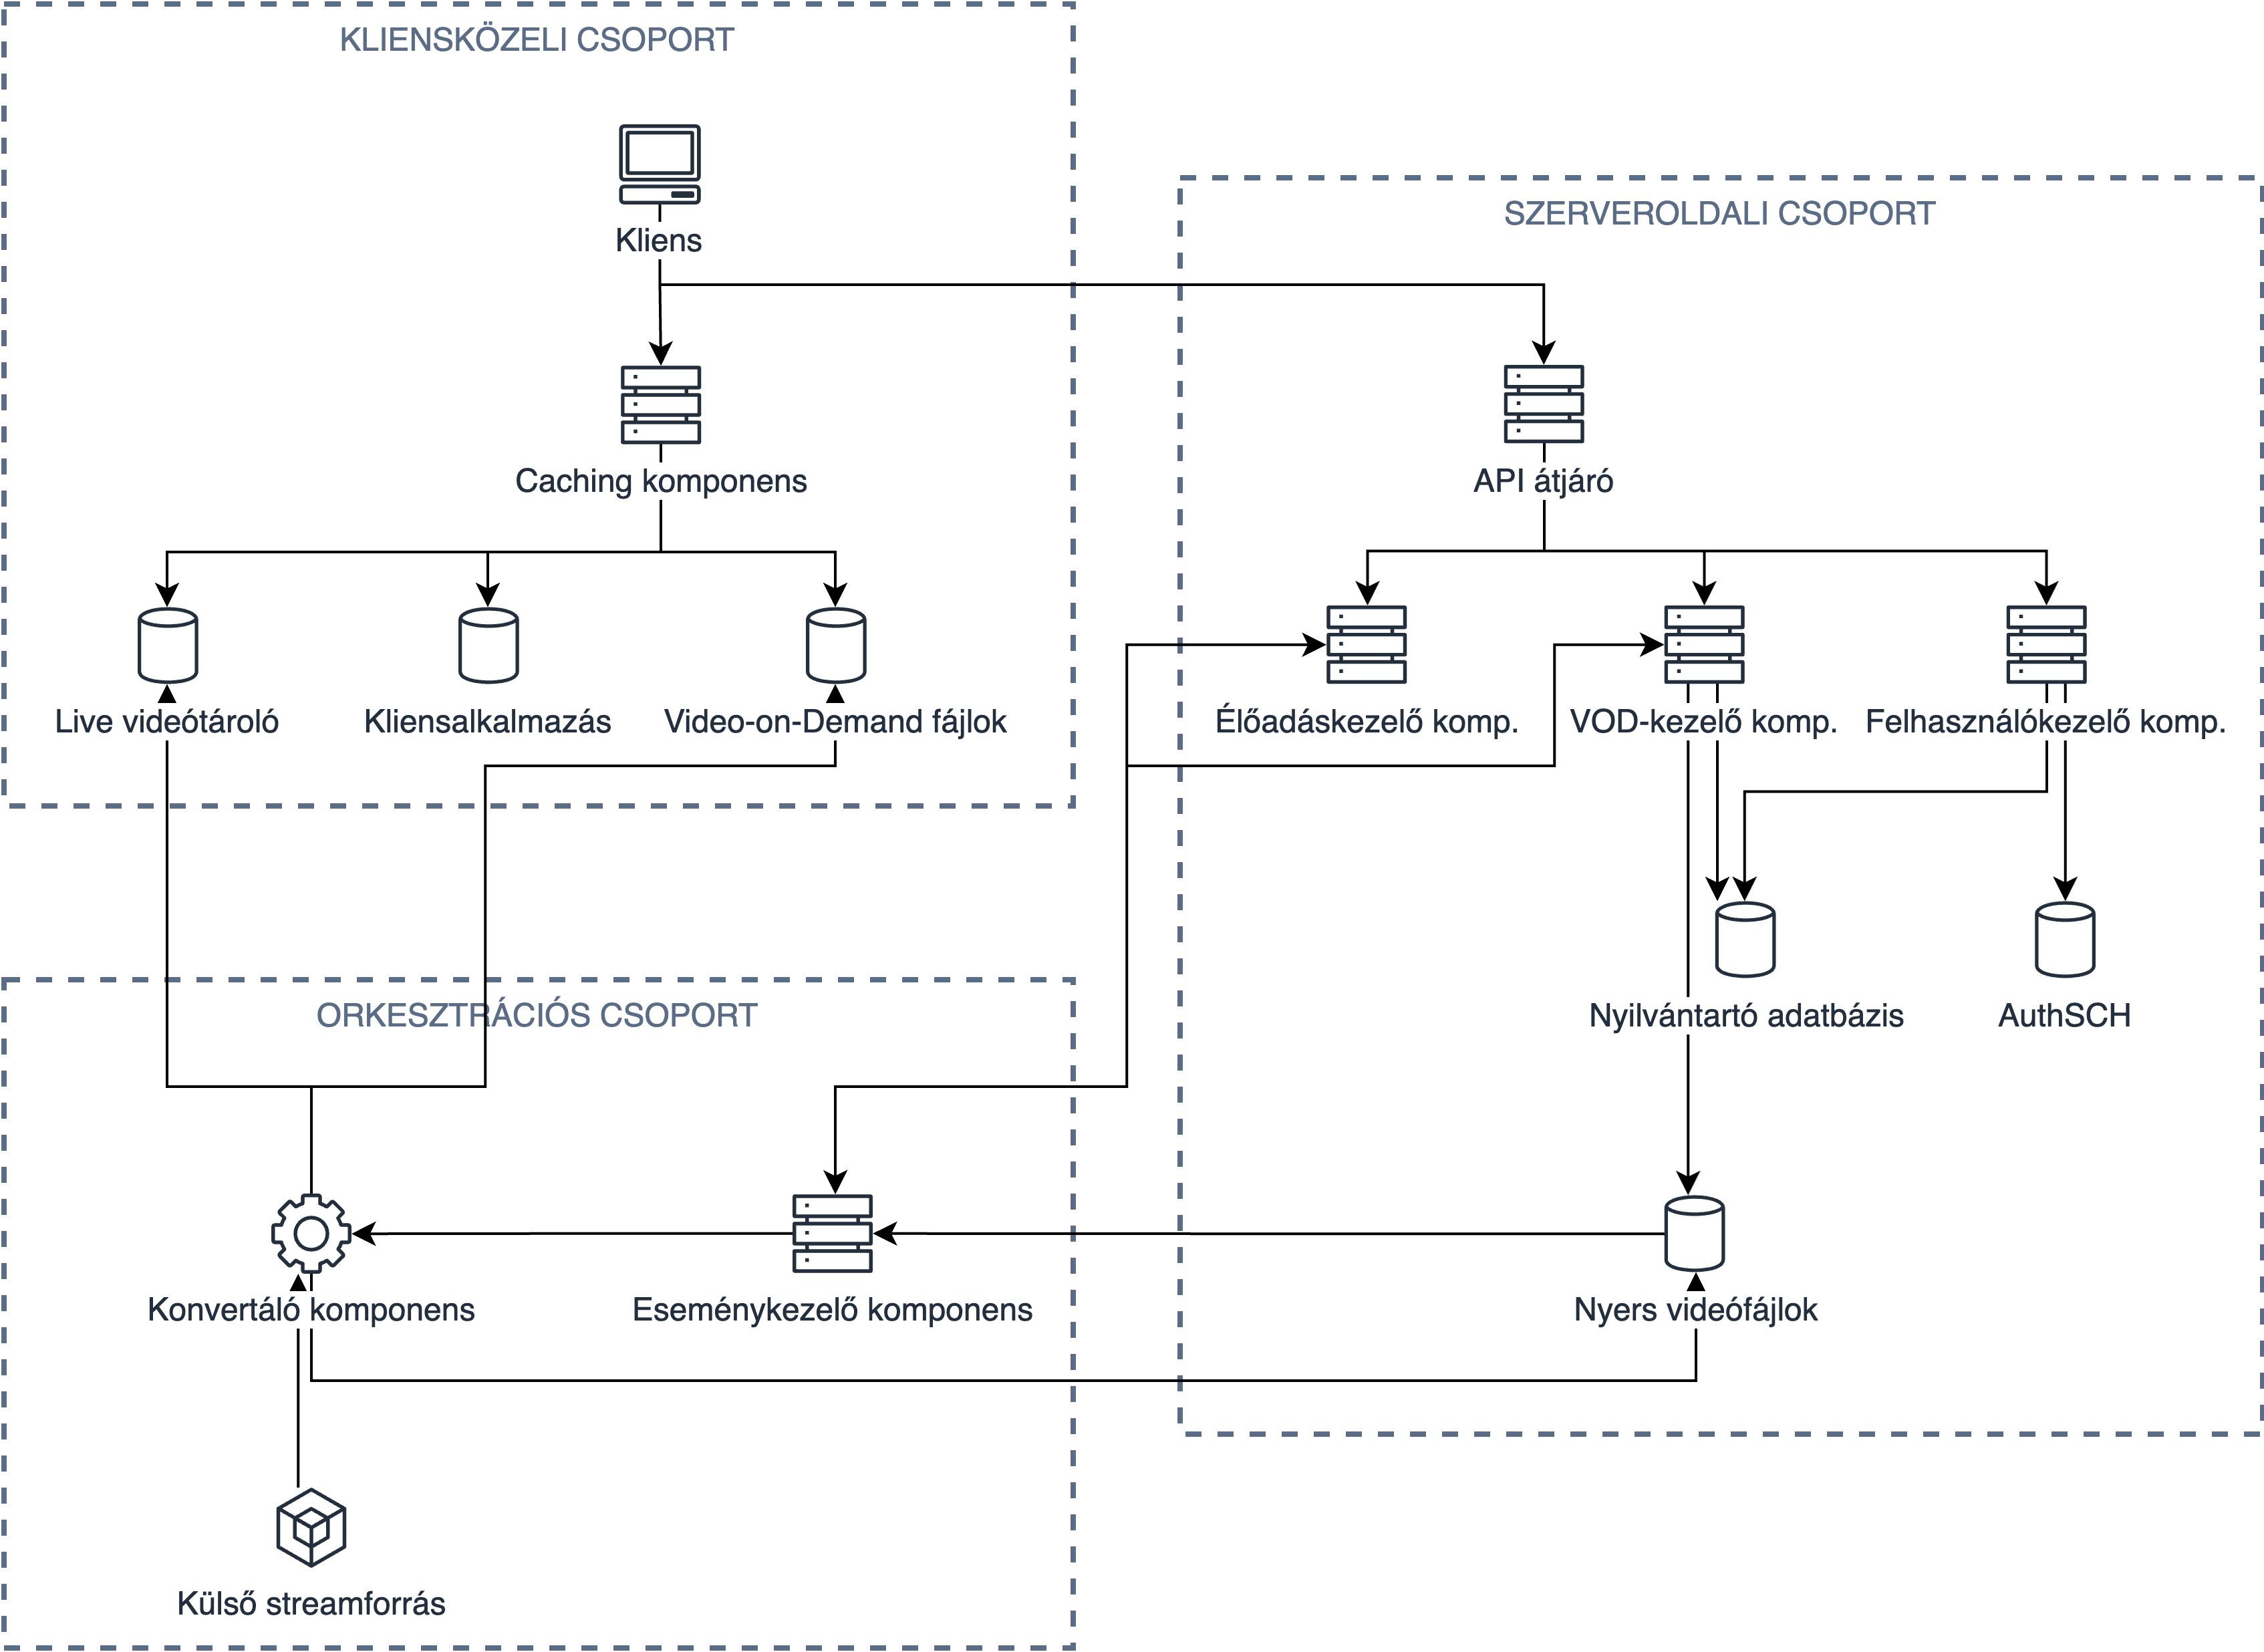
\includegraphics[width=150mm, keepaspectratio]{figures/dipterv_highlevel.png}
	\caption{Logikai felépítés a követelmények alapján.}
	\label{fig:highlevel}
\end{figure}

Megjegyzés: az itt feltüntetett komponensek élőadás-, VOD- és felhasználókezelő moduljai a későbbiekben a konkrét szoftverarchitektúrában monolit struktúrában egy közös szerveralkalmazásba kerültek bele, azon belül kerültek modularizálásra az üzleti logikában.

A korábbi \ref{streamref}. alfejezetben megismert protokollok közül a tervezés során az egyszerű implementáció és a jól támogatottság szempontjából a HTTP Live Streaming (HLS) protokollt választottam a VOD és live streaming fogadó oldalán. Az élő közvetítéshez a~Real-Time Messaging Protocol (RTMP) protokollt választottam, ehhez az OBS Studiót használtam a felstreameléshez.

\subsection{Összehasonlítás egy hasonló rendszerrel}

A tervek igazolásához segítségül kerestem az interneten nyílt forráskódú hasonló megoldásokat is. Megtaláltam a Technische Universität München (TUM) egy hallgatói csoportja, a TUM-Dev által fejlesztett az egyetemen is használt VOD és live streaming szolgáltatását, a GoCastot\footnote{\url{https://github.com/TUM-Dev/gocast}}. Ez a rendszer önállóan hosztolható szoftvereket komponál össze, nem felhőnatív.

A rendszerben az én megoldásaimhoz is hasonló absztrakt terveket lehet megfigyelni (\refstruc{fig:gocast}), ugyanígy HLS-sel szolgálják ki a tartalmakat (lásd \emph{TUM-Live Edge} példányok), viszont a live streamingre saját többportos workereket alkalmaznak (lásd \emph{TUM-Live-Worker} példányok), lehetőséget ad viszont saját streamerből RTMP-n keresztül feltölteni élő közvetítést, ahogy én is megvalósítom a saját megoldásomban. Külön mikroszolgáltatás biztosítja a live és VOD streamingen kívüli funkcionalitásokat, a TUM\leavevmode\hbox{-}Live.

Ez az ismertetett megoldás az én megoldásomhoz képest viszont nem teszi lehetővé, hogy a rendszeren kívül készült videót lehessen feltölteni és VOD-ként elérhetővé tenni rajta keresztül.

\begin{figure}[h]
	\centering
	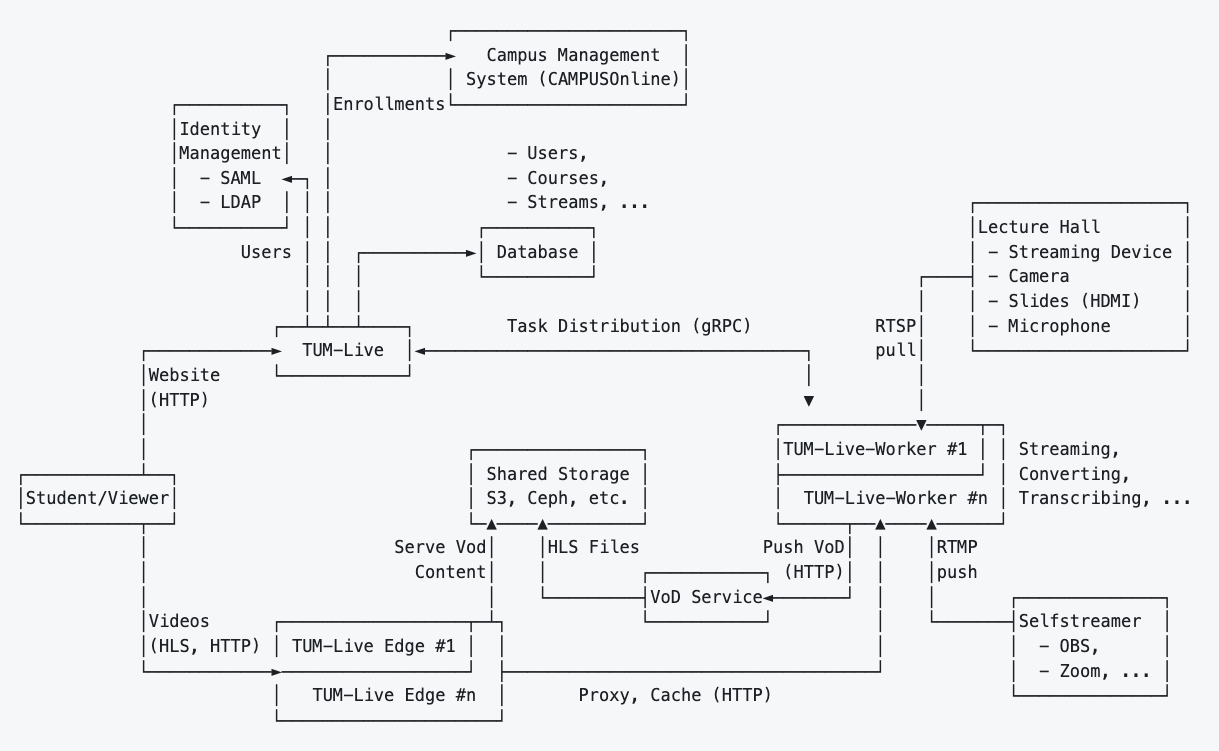
\includegraphics[width=150mm, keepaspectratio]{figures/gocast.png}
	\caption{A GoCast architektúrája a dokumentációból.}
	\label{fig:gocast}
\end{figure}

\section{Fizikai felépítés AWS-re specializáltan}

A rendszert az átlátható kezelés érdekében az AWS-felhőben egy erre külön készített AWS-fiókba helyeztem, így terveztem meg az architektúrát is. A rendszer egyszerűsített fizikai felülnézetét, azonbelül az AWS-erőforrások összeköttetését, külső szolgáltatók integrációját jól összefoglalja az \refstruc{fig:architect}.

\begin{figure}
	\centering
	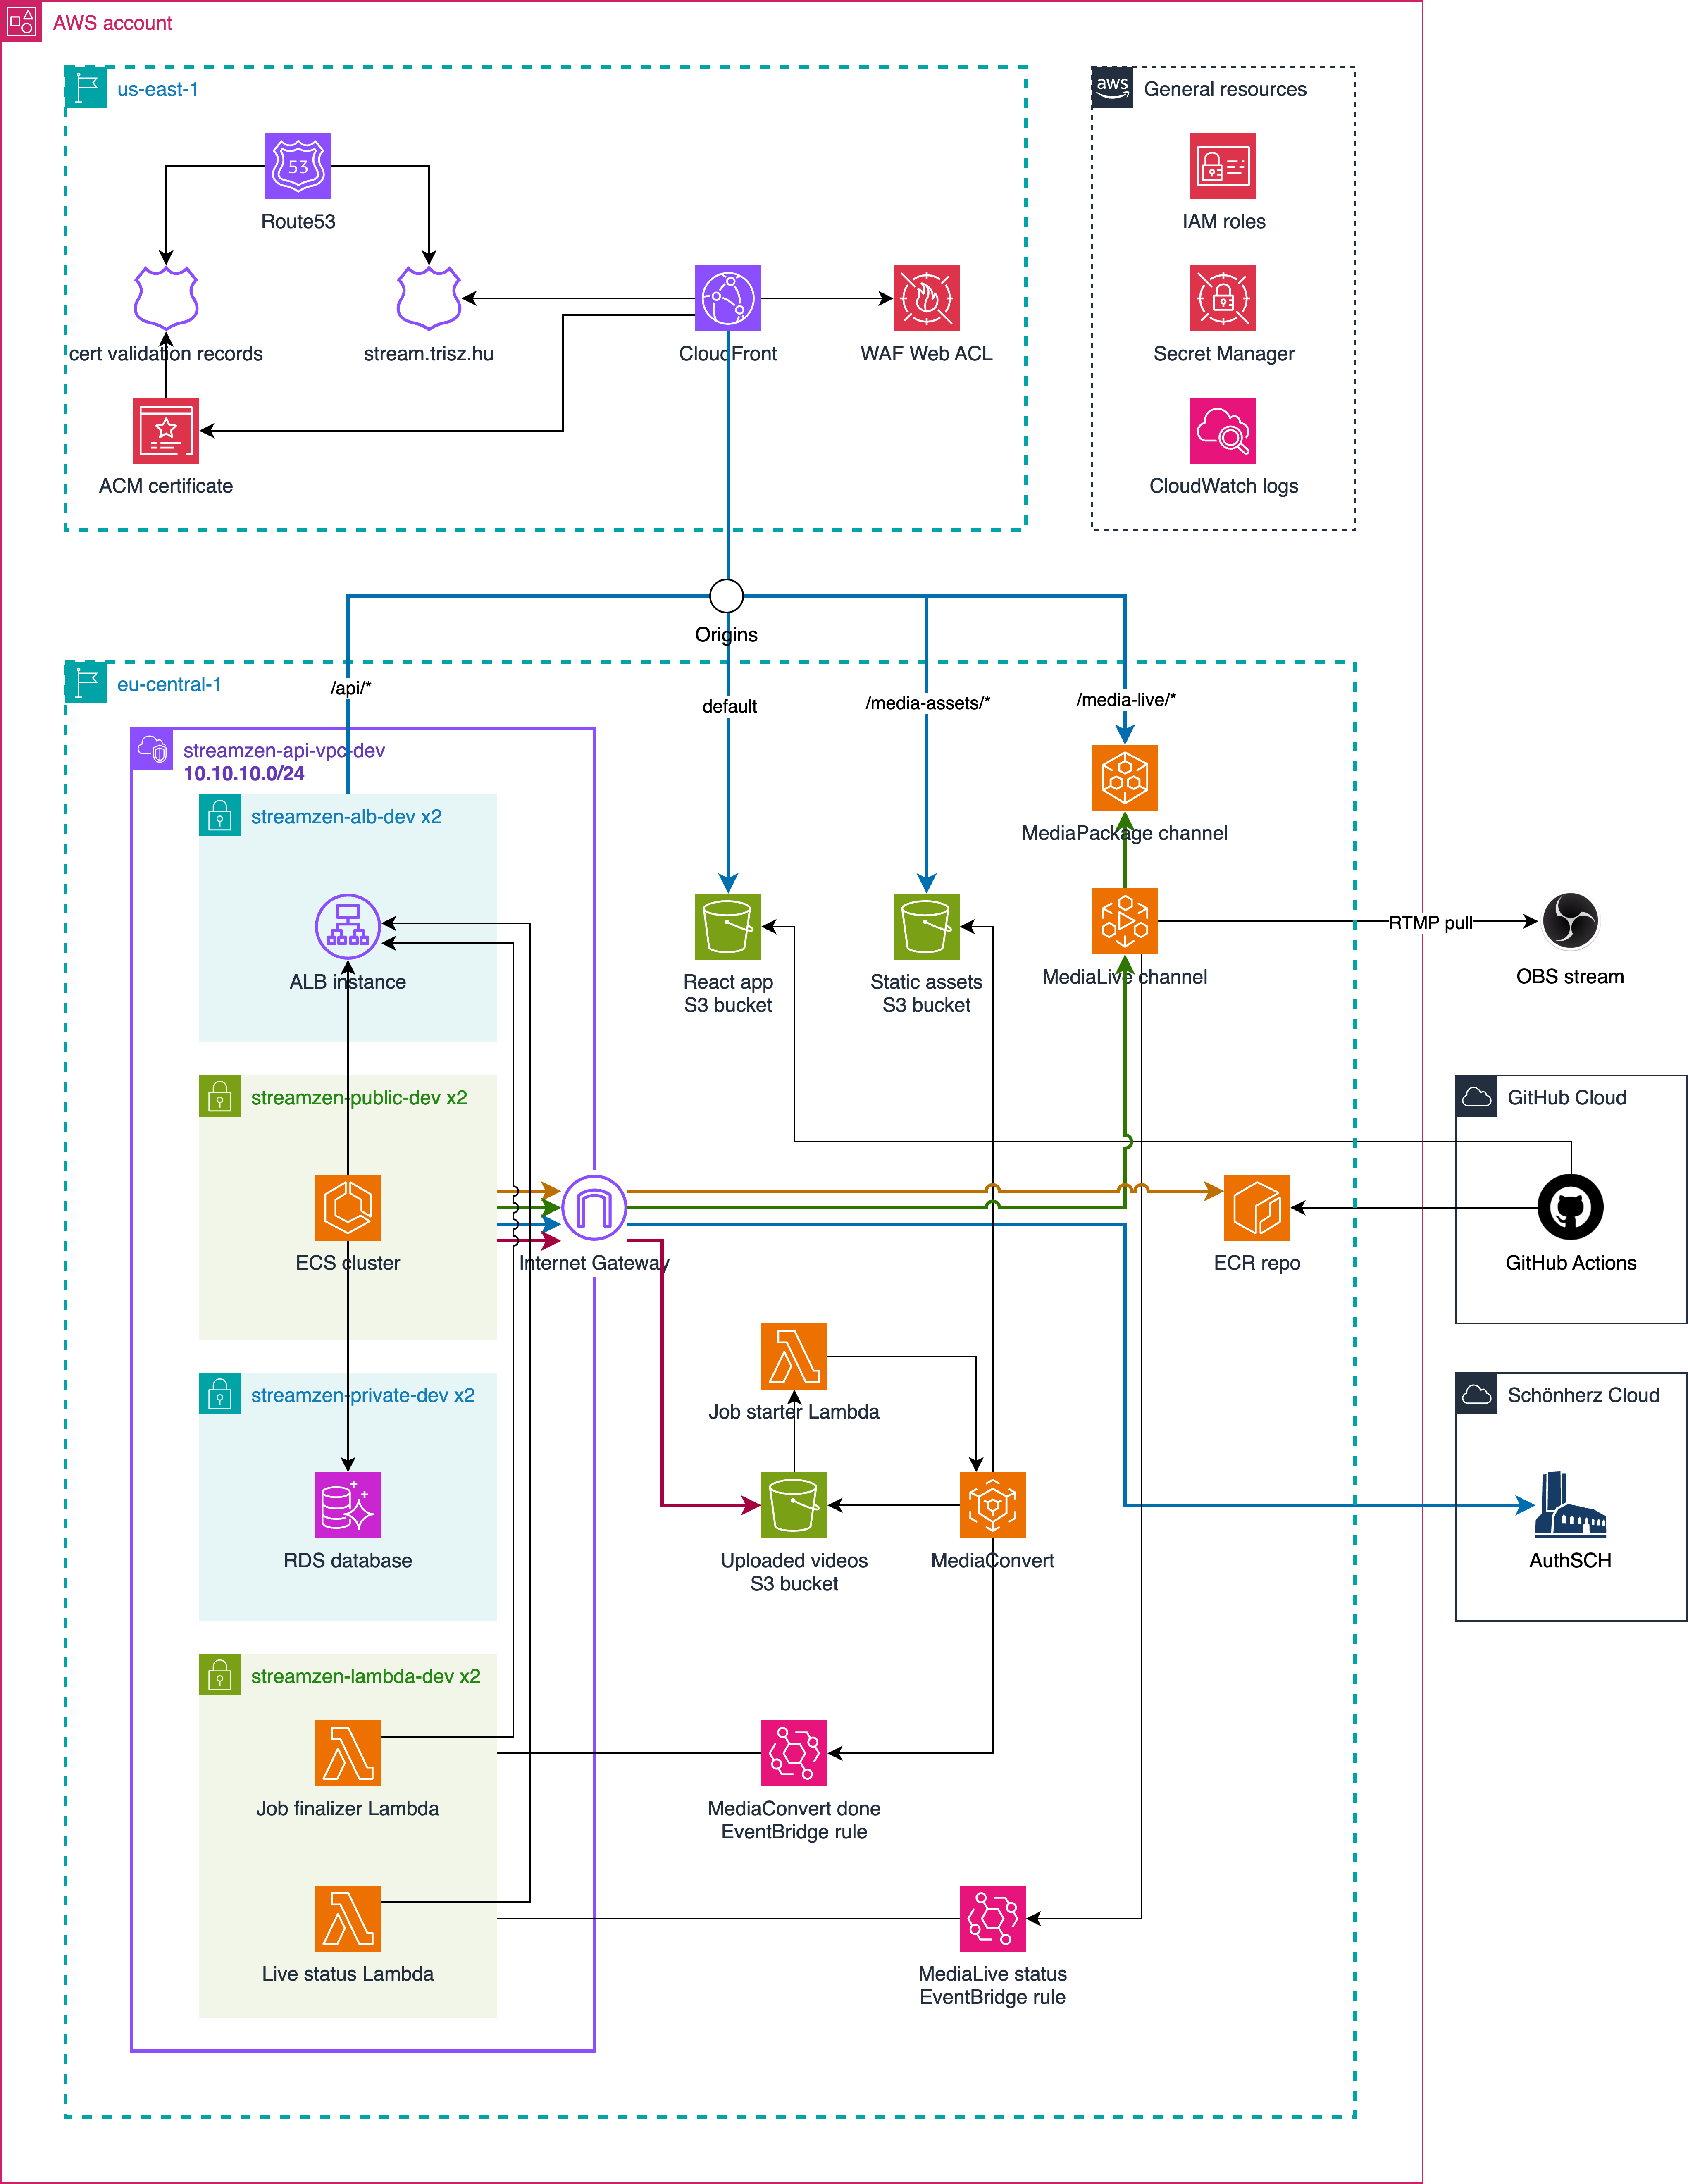
\includegraphics[width=160mm, keepaspectratio]{figures/dipterv_architect.png}
	\caption{Az AWS-fiók erőforrásainak logikai kapcsolata.}
	\label{fig:architect}
\end{figure}

Az egyes erőforrások csoportokra bonthatóak. A kliensközeli csoportot a CloudFront CDN szolgálja ki, készítettem számára egy \url{stream.trisz.hu} domén alatti Route 53 DNS\leavevmode\hbox{-}zónát is, illetve egy SSL-tanúsítványt. A védelmezésre egy AWS Web Application Firewall (WAF) web Access Control List (web ACL) is bekerült a disztribúció elé. Ezen erőforrások habár fizikailag az edge szerverfarmokra kerülnek ki, logikailag őket a~\verb|us-east-1|, azaz az észak-virginiai régióban kell elhelyezni.

A disztribúció után jönnek egy új rétegben először egy ALB-példány, ez és a mögötte lakó erőforrások az \verb|eu-central-1| (frankfurti) régión belül is egy saját hálózatba, azaz AWS VPC-be kerültek. Ezenkívül videók S3-vödrét, a React alkalmazás vödrét és a~live csatornát mind külön originként tettem a disztribúció mögé, külön-külön útvonalak mintázatokra illeszkedve.

A RTMP-alapú live stream fogadását OBS Studióból a MediaLive kezeli, ami a~MediaPackage segítségével továbbítja egy csatornán a tartalmat. A VOD-tartalmakat a~MediaConvert konvertálja HLS-adatfolyamba illeszthető formátumba, a kimenetét pedig az~S3\leavevmode\hbox{-}vödörbe helyezi. A szerveralkalmazás egy Node.js-alapú web app a terveim alapján, amely NestJS keretrendszerrel kerül kialakításra, Dockerrel konténerizálom és az ECS-be telepítem, azzal menedzselem életciklusát; az ECR-be kerülnek a konténer képei. Az adatbázis egy PostgreSQL-példánnyal kerül megvalósításra, amelyet az RDS szolgáltatásban helyezek el menedzselésre.

Az orkesztrációs eseményekre Lambda-függvények reagálnak, az eseményeket központilag az EventBridge hallgatja le szabályokkal és kötteti össze a megfelelő Lambda`|függvényekkel. Felhasználásra kerülnek a biztonságos kezelésre IAM-szerepkörök, monitorozásra és naplózásra a CloudWatch Logs, illetve az érzékeny paraméterek tárolására az AWS Secrets Manager.

A kódbázis GitHubon kerül verziókezelésre, ott a CI/CD-folyamatokat GitHub Actions segítségével automatizálom a szerveralkalmazás élesítésére, a React-alkalmazás statikus fájljainak feltöltésére. Terraformot terveztem bevezetni, amely segítségével az infrastruktúrát kód formájában kezelhetem.

\subsection{Video-on-Demand kiszolgálás folyamata}

A VOD-ok kiszolgálásának folyamatát a következőképp terveztem meg. \Az+\refstruc{fig:vod1} mutatja be a VOD-tartalom feltöltésének folyamatát, ahol a szerveralkalmazás a nyers videót buffer formájában fogadja HTTPS-en keresztül a böngészőből. A webszerver az S3-vödörbe helyezi, illetve lenyugtázza az adatbázisban, hogy a konvertálási folyamat ezzel elindult. A folyamatot a felhasználói felületen a felhasználók követhetik, ahol a folyamat állapotát mutatja a szerveralkalmazás.

\Az+\refstruc{fig:vod2} mutatja be, hogy fut le a feltöltés utáni folyamat. Egy konvertálási jobot indító Lambda-függvény feliratkozik a feltöltött videókat tároló S3-vödörre, amely a feltöltés után felkonfigurál egy jobot a MediaConvert számára, megadja a forrásfájlt és az S3-vödröt, ahova majd a job után kell kerüljön a HLS-kompatibilis fájlcsomag. Egy másik Lambda-függvény, amely a MediaConvert-job állapotváltozásaira van feliratkozva, a folyamat végén értesíti a webszervert az ALB-n keresztül, hogy nyugtázza a folyamat jelenlegi státuszát.

\begin{figure}[h]
	\centering
	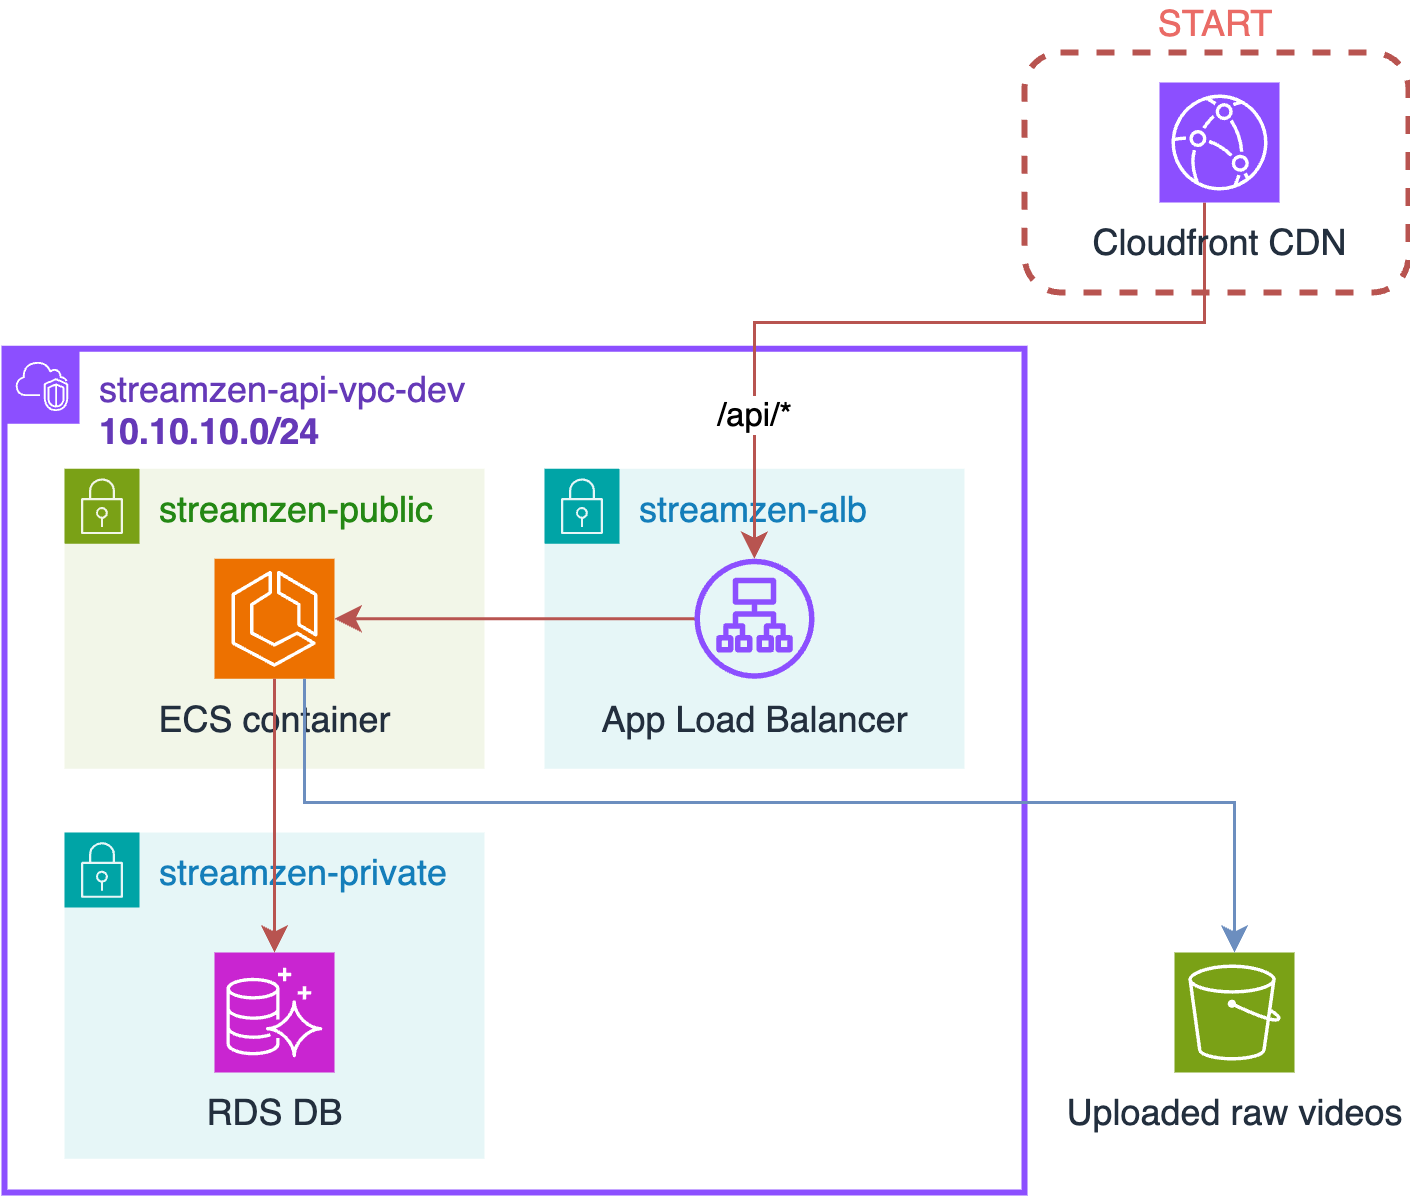
\includegraphics[height=80mm, keepaspectratio]{figures/dipterv_vod1.png}
	\caption{Folyamatábra a nyers videó feltöltéséről.}
	\label{fig:vod1}
\end{figure}

\begin{figure}[h]
	\centering
	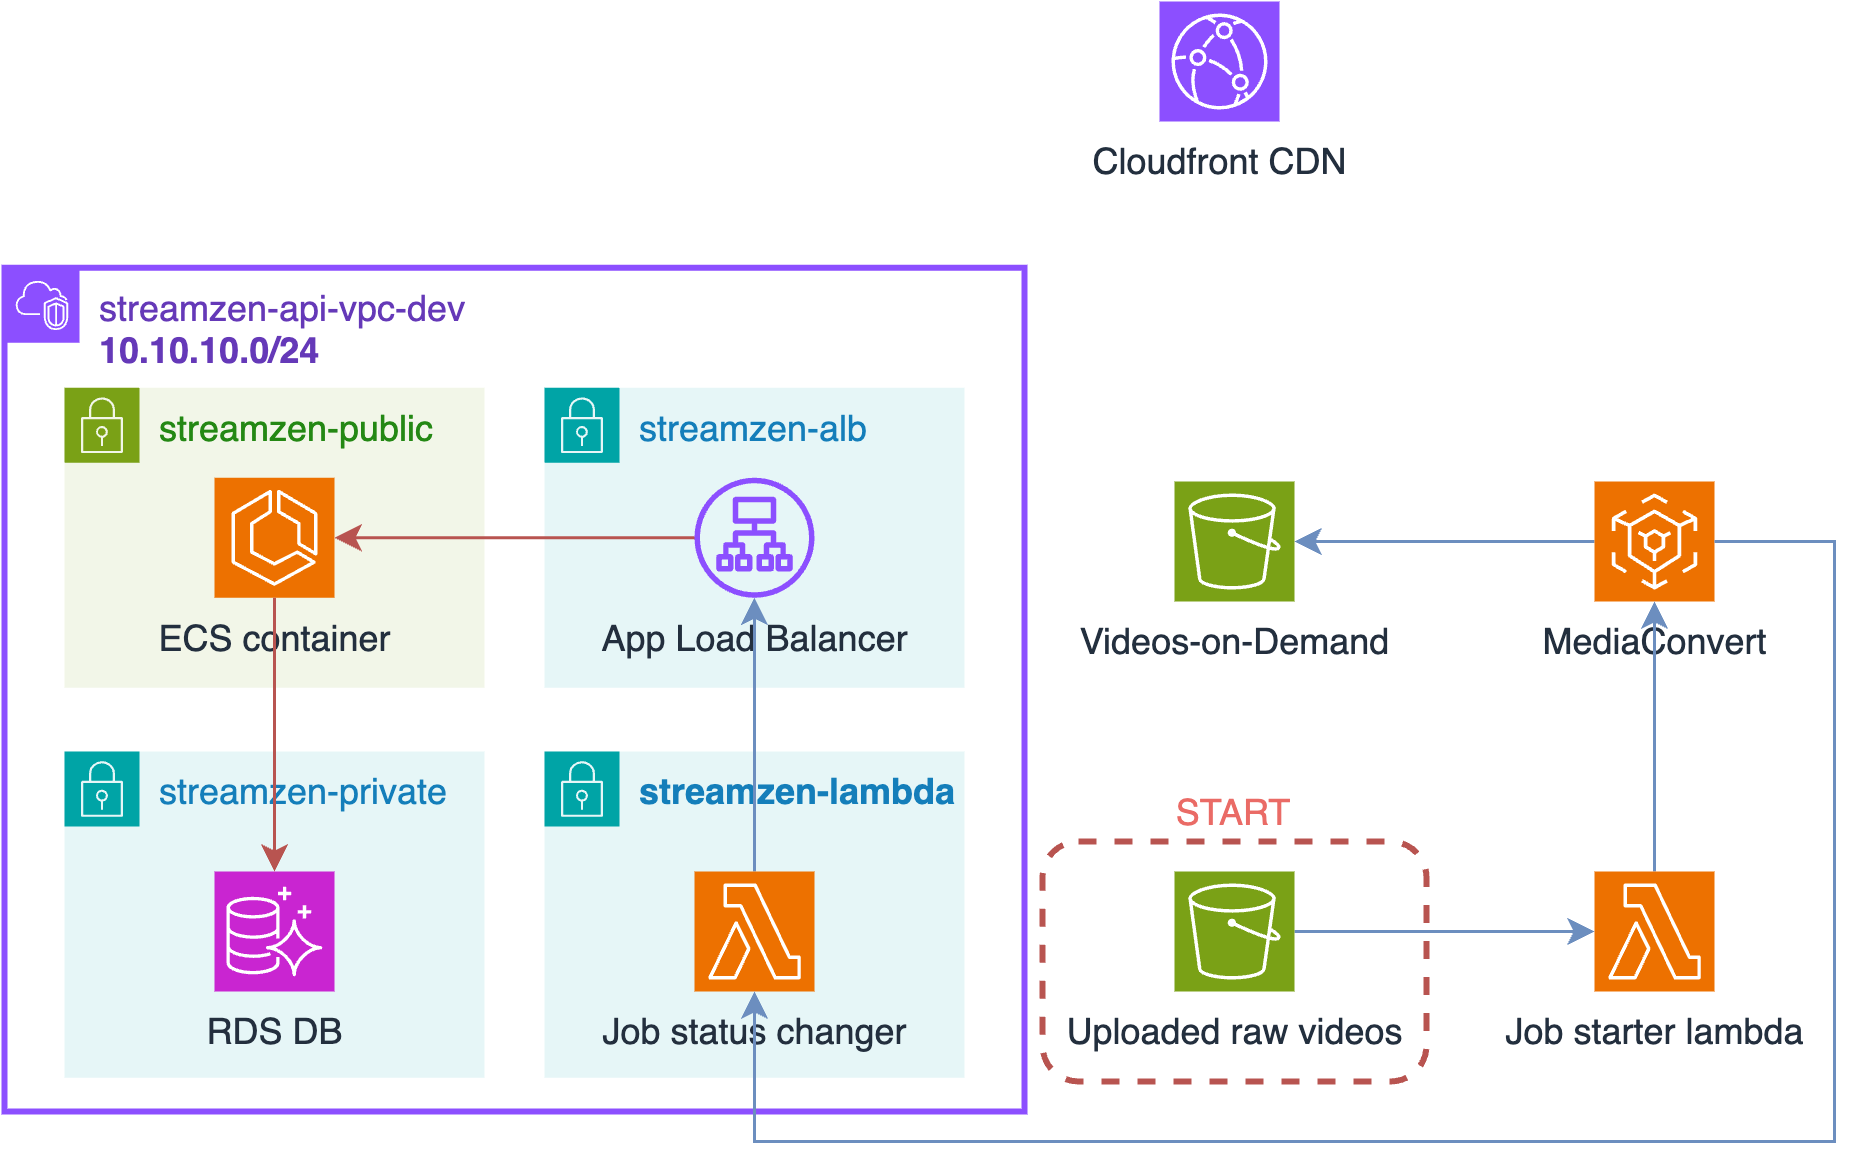
\includegraphics[height=80mm, keepaspectratio]{figures/dipterv_vod2.png}
	\caption{Folyamatábra a feltöltés utáni videófeldolgozásról.}
	\label{fig:vod2}
\end{figure}

\Az+\refstruc{fig:vod3} fejti ki egy részről, hogy hogy értesül az adminisztrátor a videó feldolgozottságának állapotáról az API-n keresztül, illetve a UI-on értesülés után mi történik, ha meg is nyitja a már streamelhető videót, amely a CloudFront-disztribúció Video-on-Demand S3-alapú originjén keresztül érhető el.

\begin{figure}[h]
	\centering
	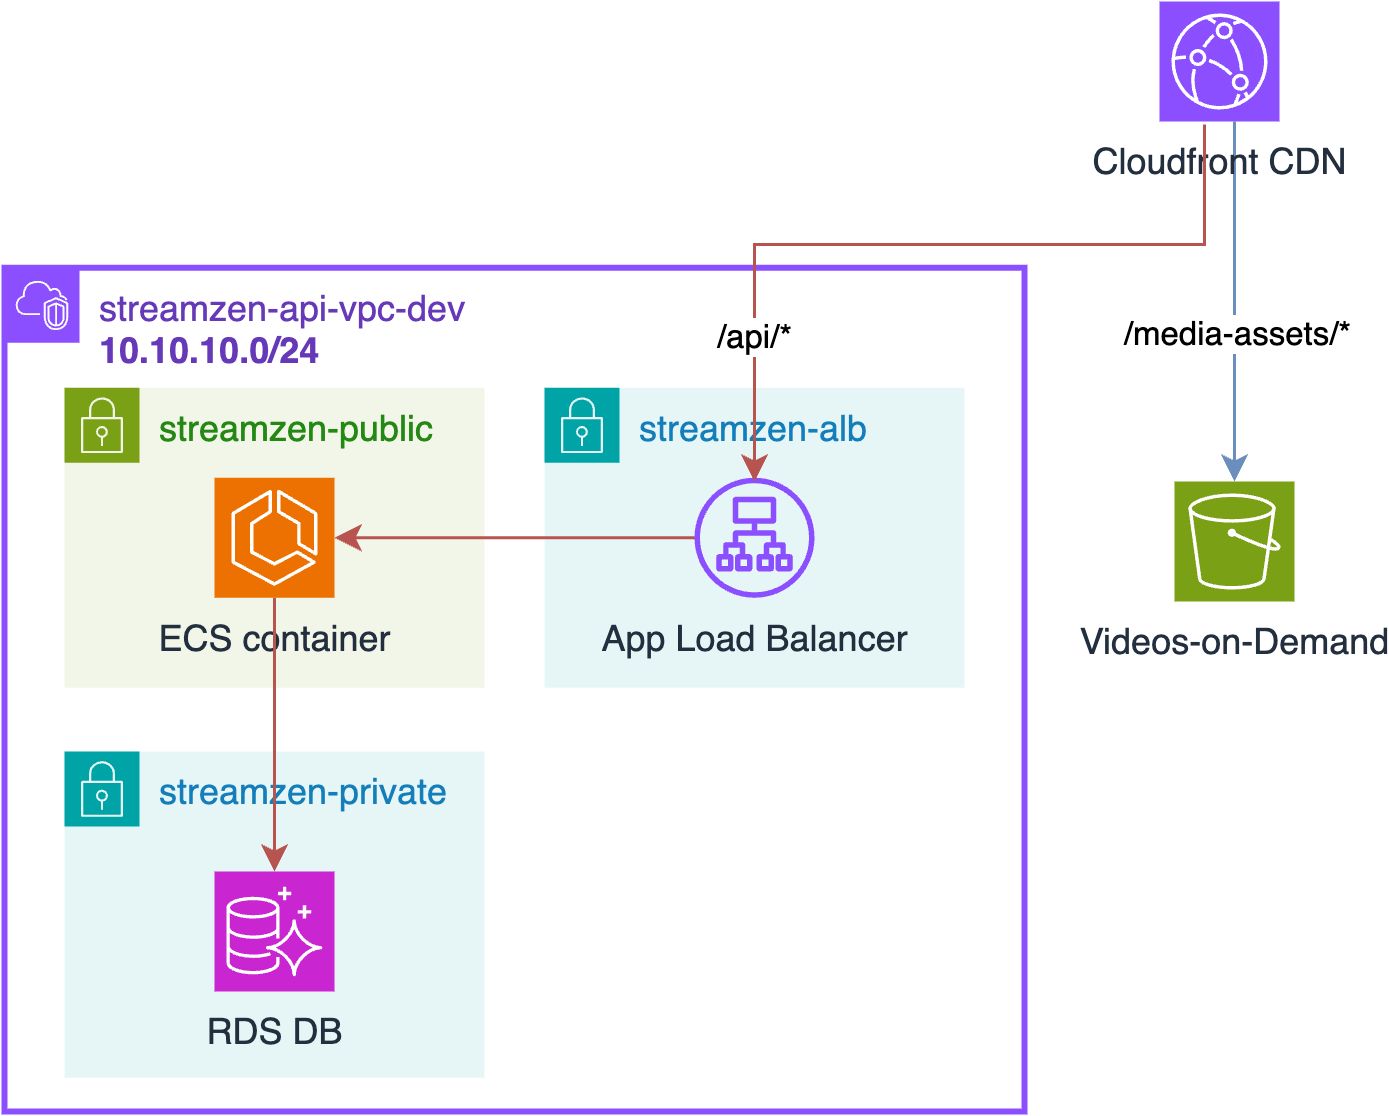
\includegraphics[height=80mm, keepaspectratio]{figures/dipterv_vod3.png}
	\caption{Folyamatábra a VOD-tartalom lejátszásáról.}
	\label{fig:vod3}
\end{figure}

\subsection{Live streaming folyamata}

A live streaming indítását mutatja be \az+\refstruc{fig:live1}. Az adminisztrátor a stúdióban gombnyomásra megnyitja API-n keresztül a live streamet, amellyel a MediaLive szolgáltatásban a csatorna is elindul, aktívan húzza RTMP-n keresztül a felcsatlakoztatott forrásból a videóanyagot.

\begin{figure}[h]
	\centering
	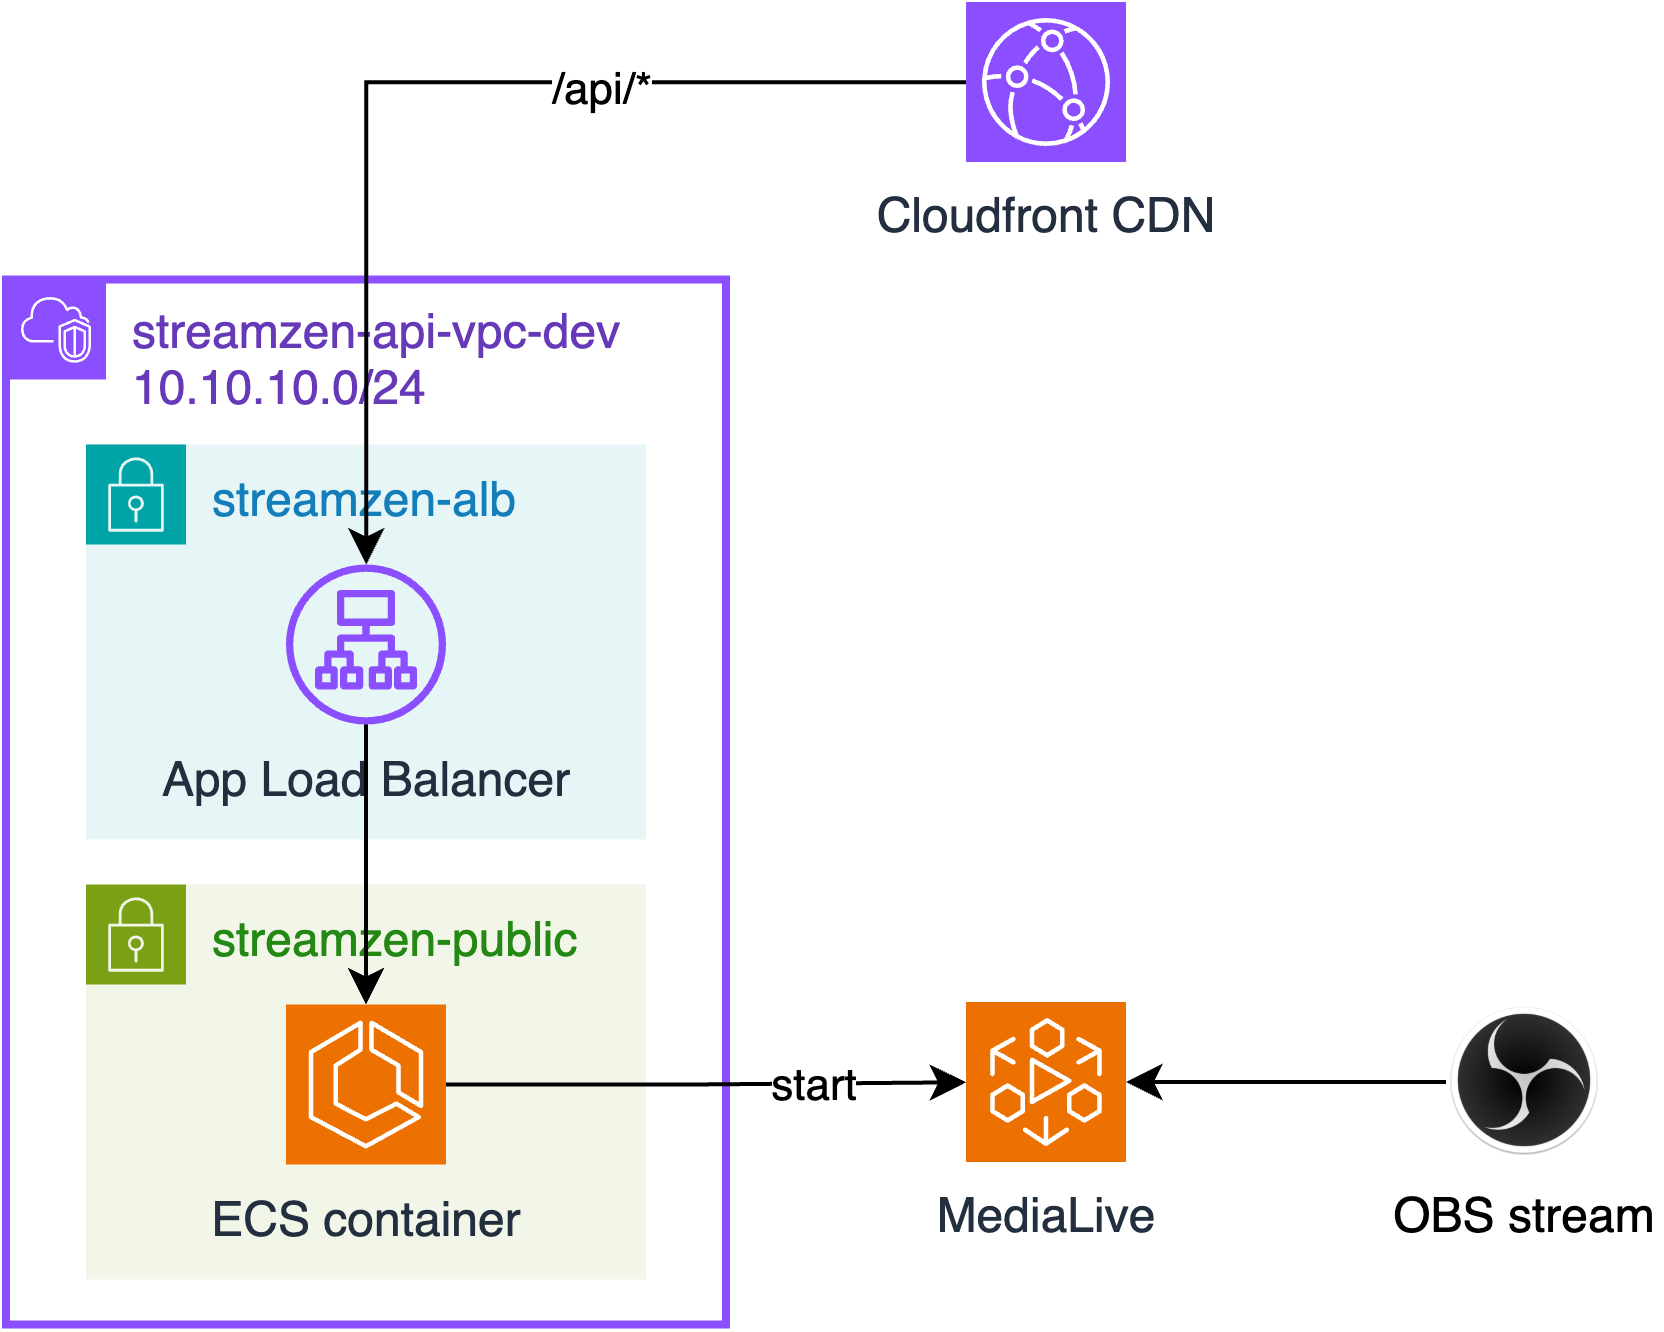
\includegraphics[height=80mm, keepaspectratio]{figures/dipterv_live1.png}
	\caption{Folyamatábra a live stream indításáról.}
	\label{fig:live1}
\end{figure}

\Az+\refstruc{fig:live2} pedig bemutatja, miután a live stream elindult, a MediaPackage-csatorna húzza át a konvertált videót a CloudFront-disztribúció elé, így ezen az originjén keresztül lesz elérhető a Cloudfront-disztribúciónak a felhasználók számára, akik a webalkalmazásban a megfelelő útvonalon érik el a live streamet.

\begin{figure}[h]
	\centering
	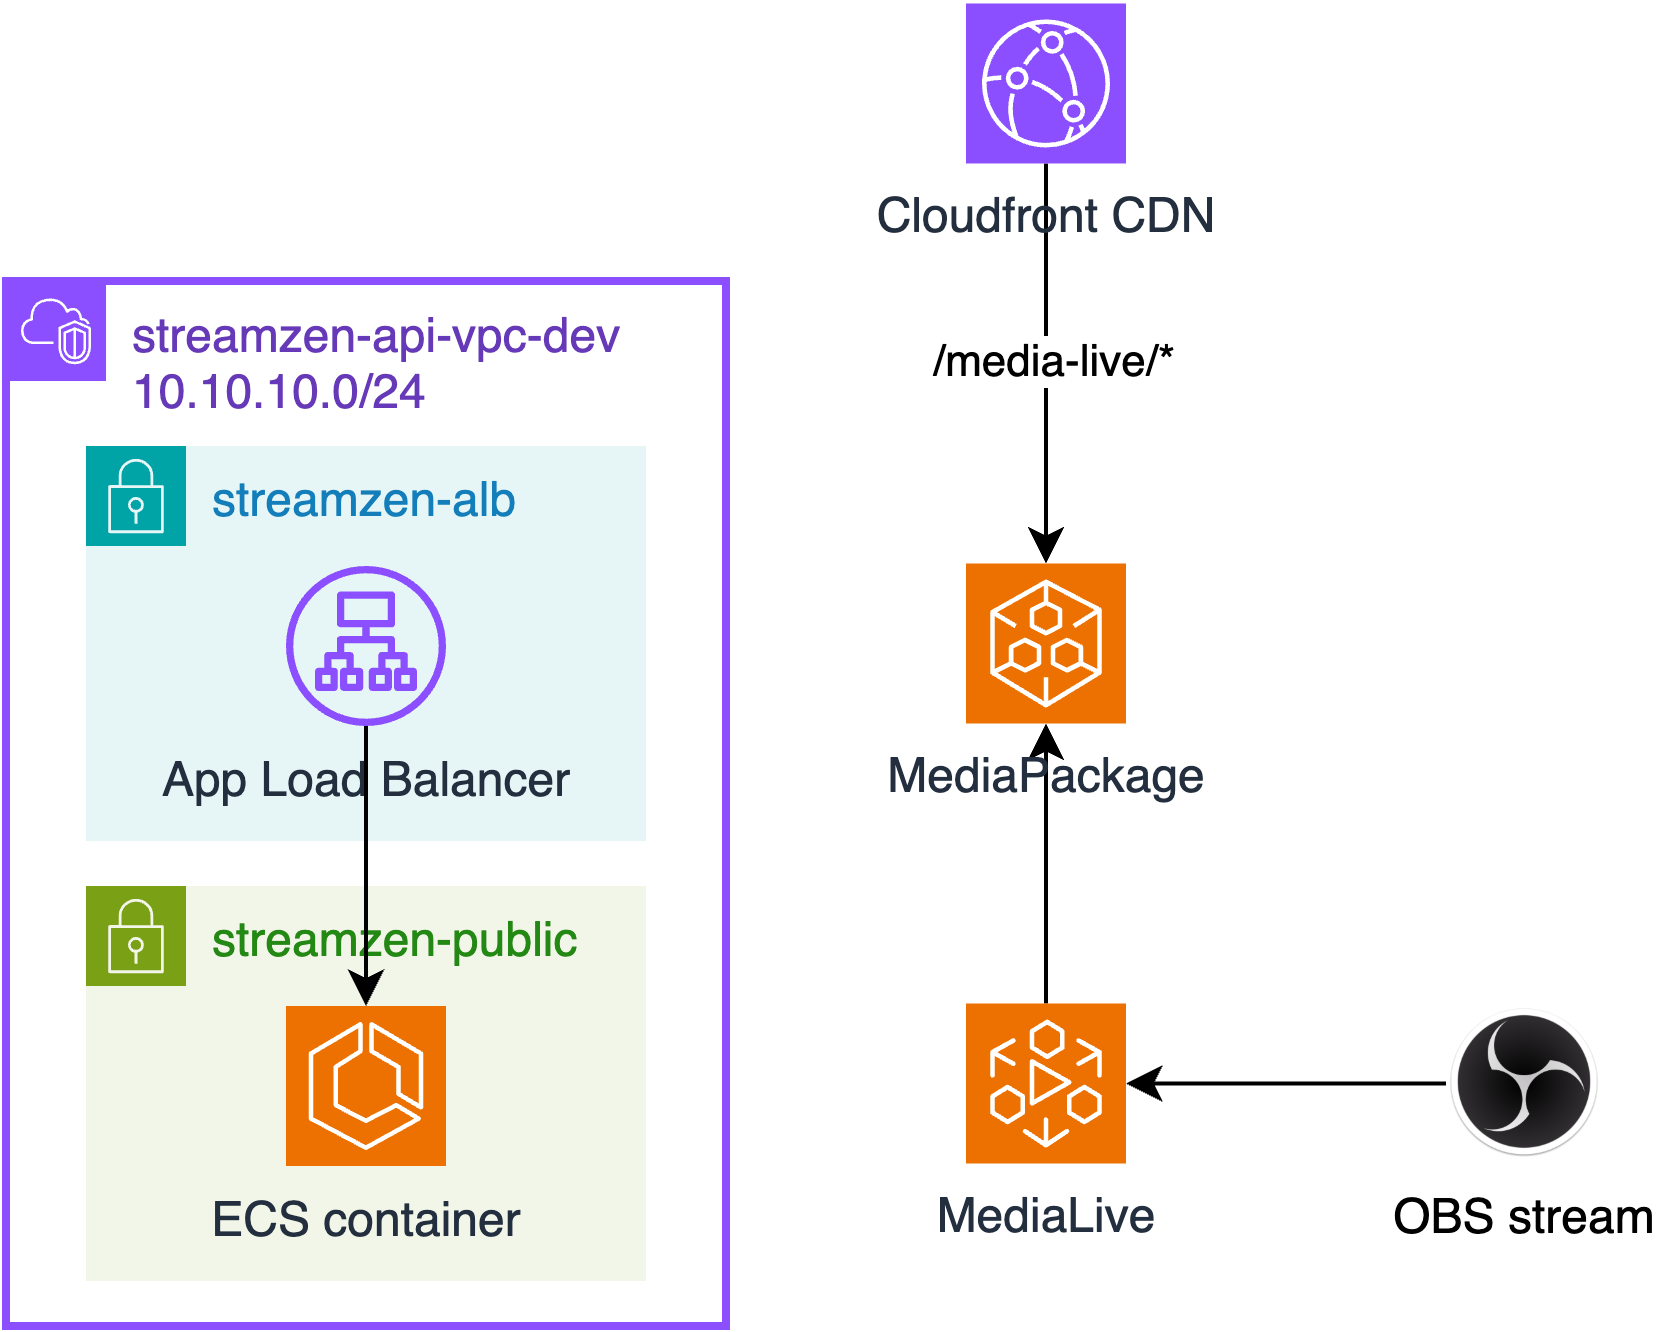
\includegraphics[height=80mm, keepaspectratio]{figures/dipterv_live2.png}
	\caption{Folyamatábra a live streamre való kapcsolódásról.}
	\label{fig:live2}
\end{figure}

\section{Konfigurációmenedzsment}\label{sec:config}

Nagyobb rendszerek tervezése igényli, hogy megfelelő konfigurációmenedzsmentet teremtsen köré a tervezőmérnök, hogy a rendszer könnyen karbantartható legyen. A Terraform lehetővé teszi az infrastruktúra építését és az annak felkonfigurálását kód formájában, a~kódban való élesítések nyomán friss és dokumentált marad az állapota is ezeknek.

Egyetlen környezetet terveztem kialakítani, egy \emph{development}, azaz fejlesztési környezetet, azonban úgy szervezve a környezet erőforrásait, hogy később akár szakaszos bevezetéssel (\emph{rollout}) újra élesíthető lehessen egy másik (pl. \emph{production}, azaz gyártási) könyezetre. A Terraform-modulokat egy befoglaló Terragrunt gyökérmodulba szerveztem, a \verb|streamzen-core| mappába. Az erőforrásokat igyekeztem olyan módon elnevezni, hogy azok tartalmazzák a \verb|streamzen| prefixet és a környezet nevét, például \verb|dev| is tartalmazzák, hogy könnyen lehessen azonosítani őket a későbbiekben. Az erőforrások alapvetően az ``eu-central-1'' régióban helyezkedtem el, a globális erőforrások kivételével.

Terraformban menedzselt infrastruktúra tipikus életciklusa áll a kódból származó tervek előállításából (plan), annak manuális átolvasásából, majd pedig a változtatások aktiválásából (apply). Az automatizálás érdekében GitHub Action-munkafolyamatokba terveztem szervezni az élesítési tervek előnézetének generálását -- amely a \verb|terraform| \verb|plan| parancs kiadásával kezdeményezhető --, ami minden Pull Request (PR) UI-ján kommentként kerül hozzáadásra a PR-hez, viszont a tervek élesítését (erre használt parancs a \verb|terraform| \verb|apply|) saját kézzel a saját parancssoromból terveztem megtenni, tekintettel arra, hogy csupán egyedül dolgoztam a kódbázissal.

Hogy az AWS-fiók erőforrásaihoz hozzáférést kaphassanak az egyes munkafolyamatok, azok számára OpenID Connect (OIDC) felállításával terveztem az erre szánt AWS`|szerepkör felvételét megvalósítani (\refstruc{fig:githuboidc}).\cite{githuboidc}

A szerveralkalmazás egységként való kezelése érdekében és a könnyű telepíthetőségért -- ahogy ezt a nem funkcionális követelmények is megkívánták -- konténerizálni terveztem a~Node.js-szerveralkalmazást Docker-konténerbe való komponálással, a buildelési folyamatot Dockerfile-lal kívántam megvalósítani hozzá. GitHub Action került alkalmazásra a~buildelt Docker-konténerkép ECR-be való automatizált feltöltésére (\refstruc{fig:ecr}), a~React-kód buildelésére és S3-vödörbe való feltöltésére.

\vspace{1cm}

\begin{figure}[h]
	\centering
	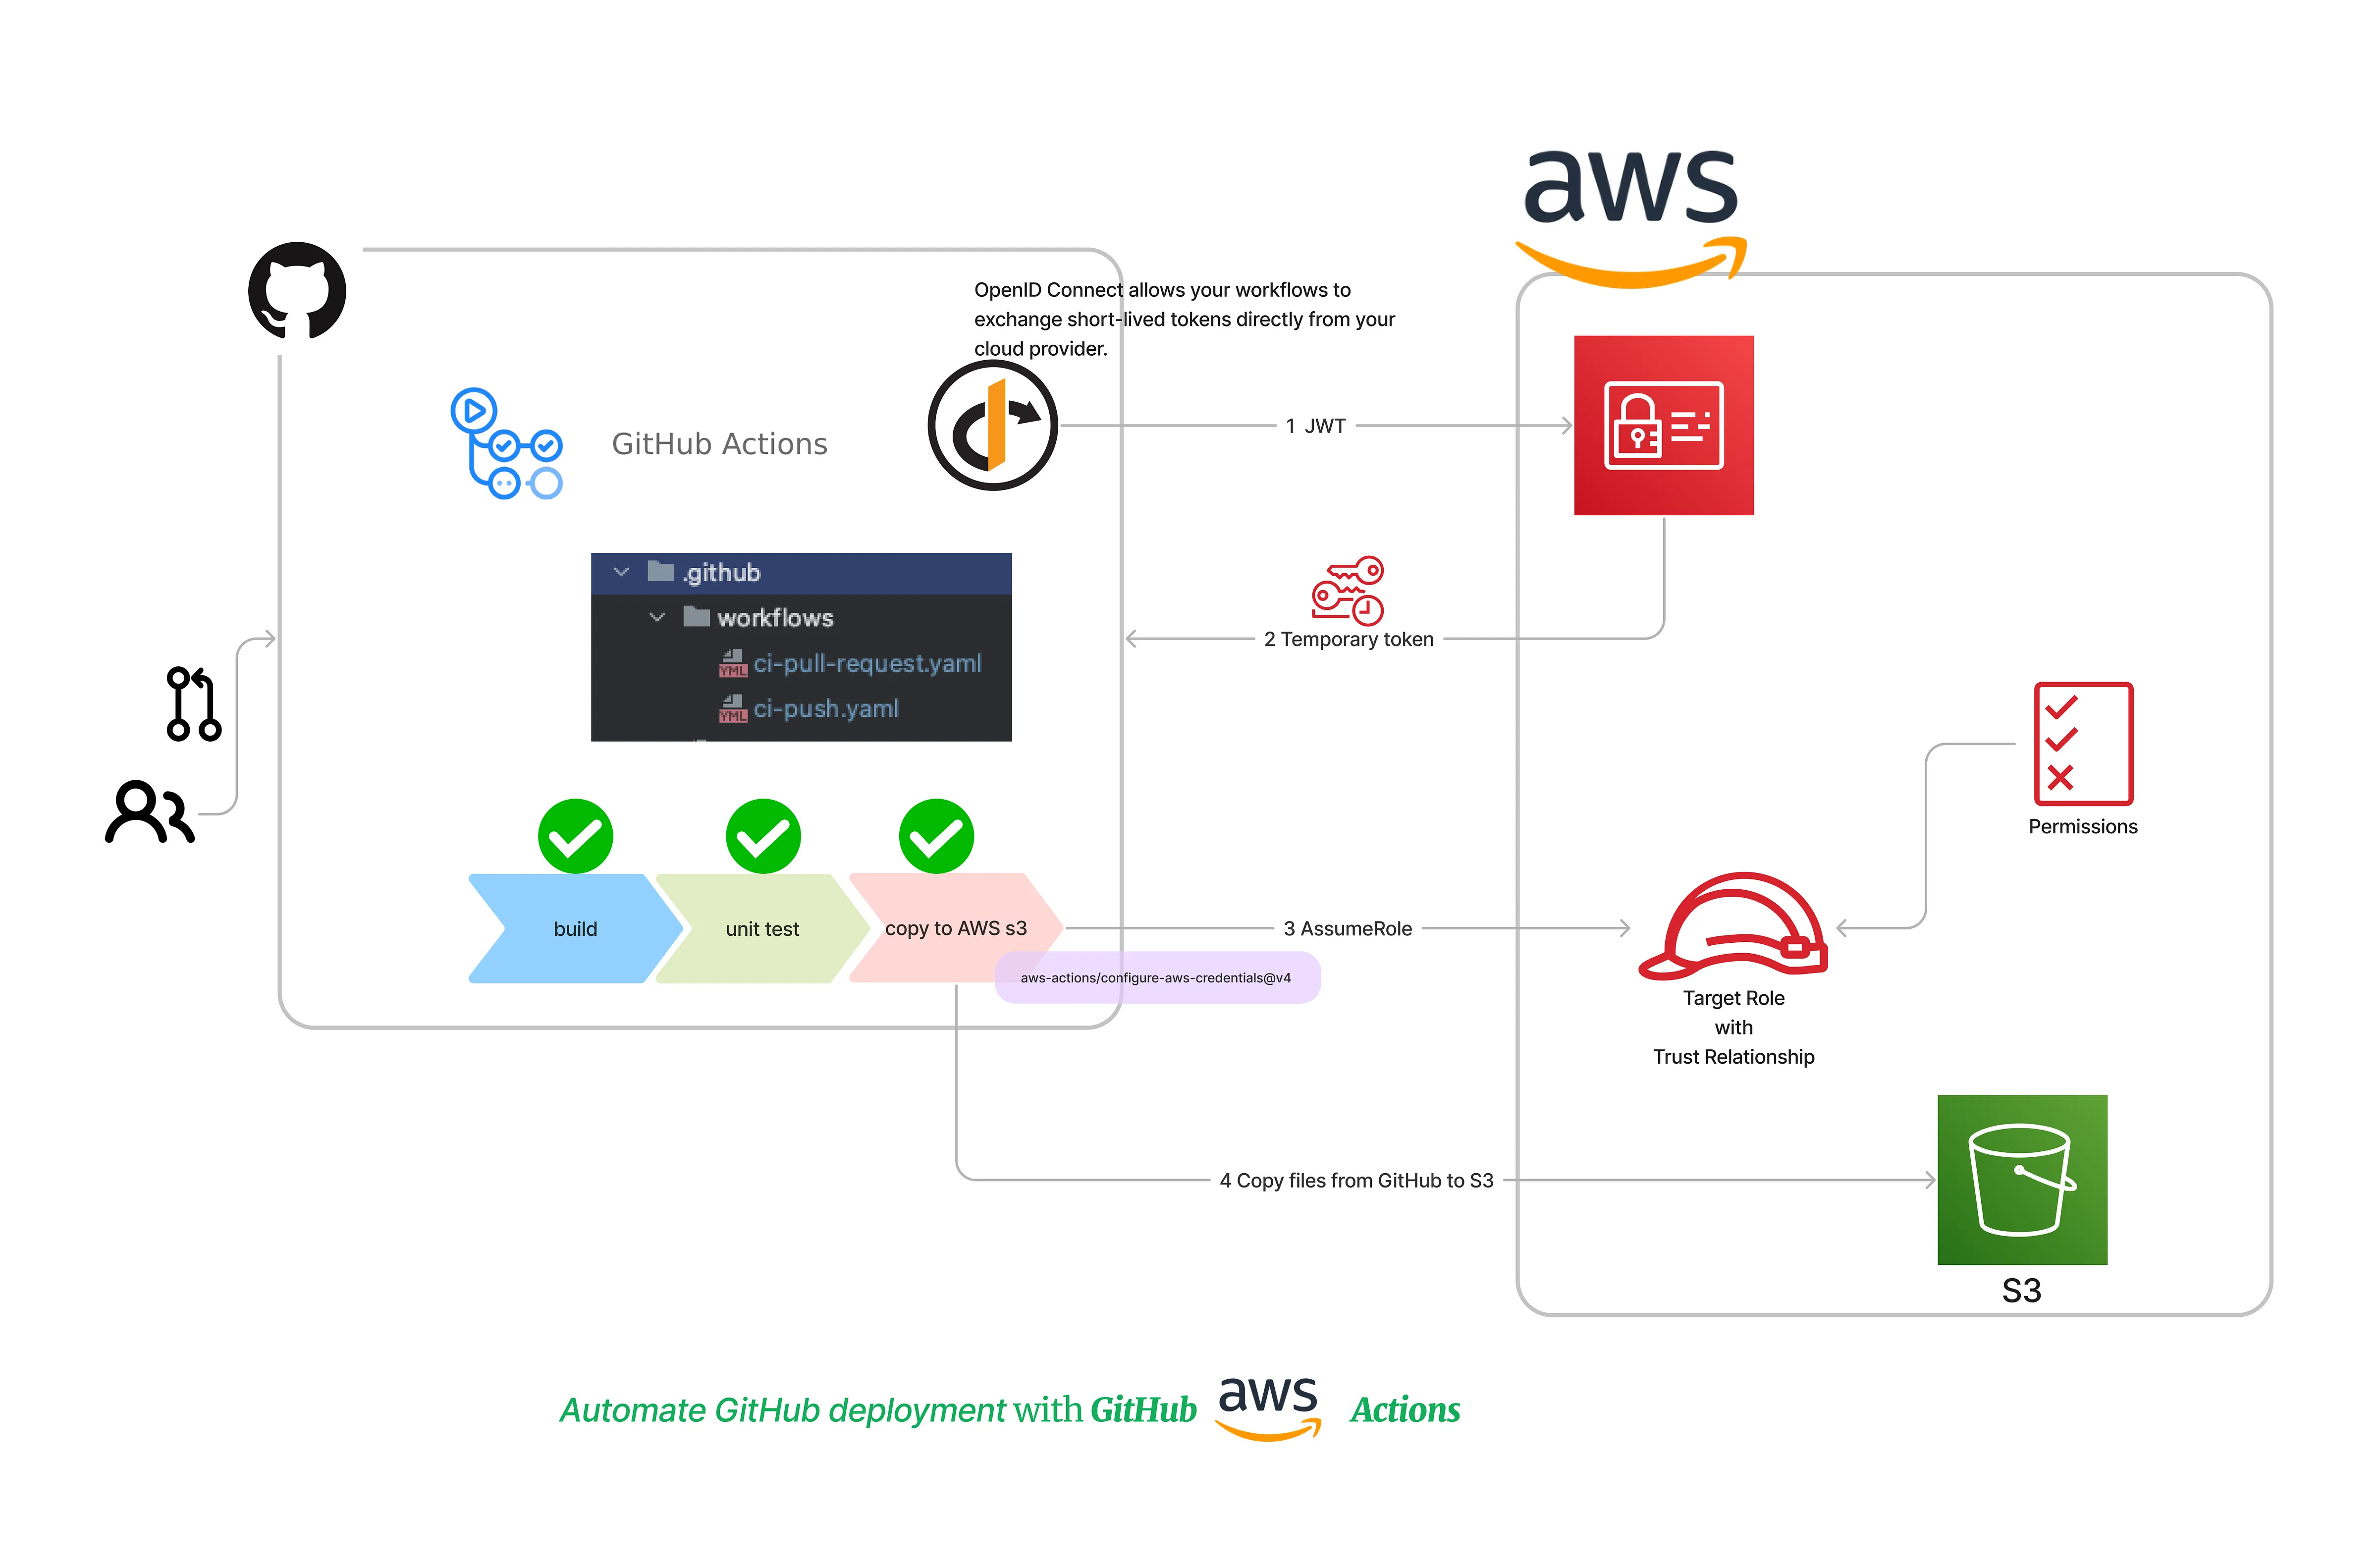
\includegraphics[width=150mm, keepaspectratio]{figures/githuboidc.png}
	\caption{Workflow autorizálása AWS-szerepkörre OIDC-val.}
	\label{fig:githuboidc}
\end{figure}

\vspace{1cm}

\begin{figure}[h]
	\centering
	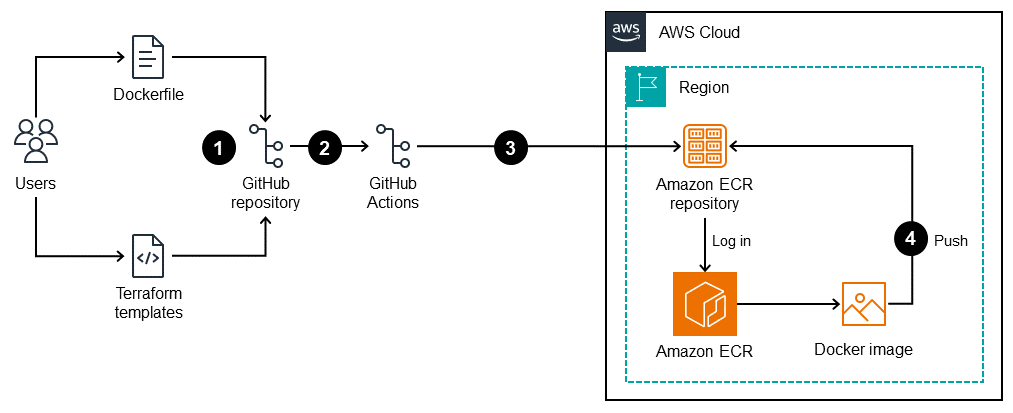
\includegraphics[width=150mm, keepaspectratio]{figures/ecr.png}
	\caption{Folyamatábra a Docker-kép ECR-be feltöltéséről.}
	\label{fig:ecr}
\end{figure}

\section{A projekt felépítése}

A projekt kódja ``monorepo'' alapokon nyugszik egy GitHub repositoryban. A TypeScript-alapú projektekre bő eszköztárat és könnyű kezelést biztosít a~Visual Studio Code (röviden VSCode\footnote{\url{https://code.visualstudio.com/}}). A teljes kódbázis gyökérében található \verb|streamzen.code-workspace| fájl VSCode-ban való megnyitása segít átlátni a hat alprojektet:

\begin{itemize}
	\setlength{\itemsep}{1pt}
  \setlength{\parskip}{0pt}
  \setlength{\parsep}{0pt}
	\item \verb|client| mappa: React-alapú statikus SPA-projekt kódbázisa.
	\item \verb|server| mappa: Node.js-alapú szerveralkalmazás kódbázisa.
	\item \verb|infra-bootstrap| mappa: Terraform-alapú infrastruktúra kódbázisa, amely a csővezetékhez szükséges erőforrásokat állítja fel. Egyszer futtatandó, ez állítja fel az~S3`|vödröt a Terraform-állapot tárolására és a jogosultságokat a CI/CD-csővezeték OIDC-n keresztüli kapcsolódásához az AWS-fiókba.
	\item \verb|infra| mappa: Terraform-alapú kódbázis minden más erőforrásra.
	\item \verb|.github| mappa: GitHub Action-munkafolyamatok kódbázisa.
	\item \verb|perftesting| mappa: A teljesítménytesztelést végző JavaScript-kódbázis.
\end{itemize}

\chapter{Kliensközeli komponensek implementációja}

A következőkben részletezem a klienseket kiszolgáló infrastrukturális komponensek konfigurációját, valamint a legfelső megjelenítési réteg szoftveres komponenseinek implementációját. A forgalom először a CDN-nel ütközik, amelyen keresztül lesznek elérhetőek a~statikus weboldal erőforrásai, valamint a média-erőforrások csatornái.

\section{A CDN és a hozzácsatolt erőforrások}

A CDN és az ahhoz tartozó erőforrások jelentik az első belépési pontját egy a rendszerhez intézett kérésnek. A rendszer és a CDN -- azaz a CloudFront-disztribúció -- számára a~\verb|stream.trisz.hu| doménnevet rendeltem, amelyet a saját \verb|trisz.hu| doménem aldoménjeként jegyeztem be a~Route 53 szolgáltatásban egy külön DNS zónaként. A böngészőből, azaz kívülről indított kérések minden esetben a DNS feloldásával kezdődnek, a~Route 53 névszervereire oldódik fel, ezzel szerzi meg a kliens az IP-jét a CloudFront edge szerverfarmjának. A CloudFront-disztribúcióknak különleges CNAME rekordjaik vannak, biztosítják hogy a kliens a legközelebbi edge szerverfarmhoz csatlakozhasson, a konkrét működést az AWS elrejti a háztető alatt előlünk. A biztonságos, HTTPS-alapú szerver--kliens kommunikációt a CloudFront-disztribúcióhoz tartozó SSL-tanúsítvánnyal biztosítja a rendszer. A tanúsítványt az AWS Certificate Manager szolgáltatásban generáltam és kezeltem, amely automatikusan megújítja a lejáró tanúsítványokat, amennyiben a doménhez tartozó DNS-zónát a Route 53 szolgáltatásban -- azaz az AWS szolgáltatásában kezeljük.

A CloudFront-disztribúcióhoz hozzácsatoltam egy WAF ACL-t, amely a webalkalmazás szintű tűzfal szerepét tölti be. Minden kérést ez a Layer 7 rétegbeli logika szűri meg. Mivel nem volt élő forgalomra készítve az alkalmazás, így egy egyszerű AWS menedzselte szabályt tettem csak rá a WAF-ra demonstrációképp, amely megvizsgálja a kérést, hogy tartalmaz-e SQL injection támadást vagy egyéb megszokott webalkalmazásokra jellemző ilyen jellegű támadást (pl.: ismert kihasználható URI`|útvonalak, Java webalkalmazásokra jellemző exploitok) -- a szabálycsoportot név szerint \verb|AWSManagedRulesKnownBadInputsRuleSet| név alatt tartja számon az AWS WAF.

Az edge-en kerül kiértékelésre a kapott kérés útvonala (angolul \emph{path}) alapján az, hogy melyik origin felé kell továbbítsa a disztribúció a kérést.

\begin{figure}[h]
  \centering
  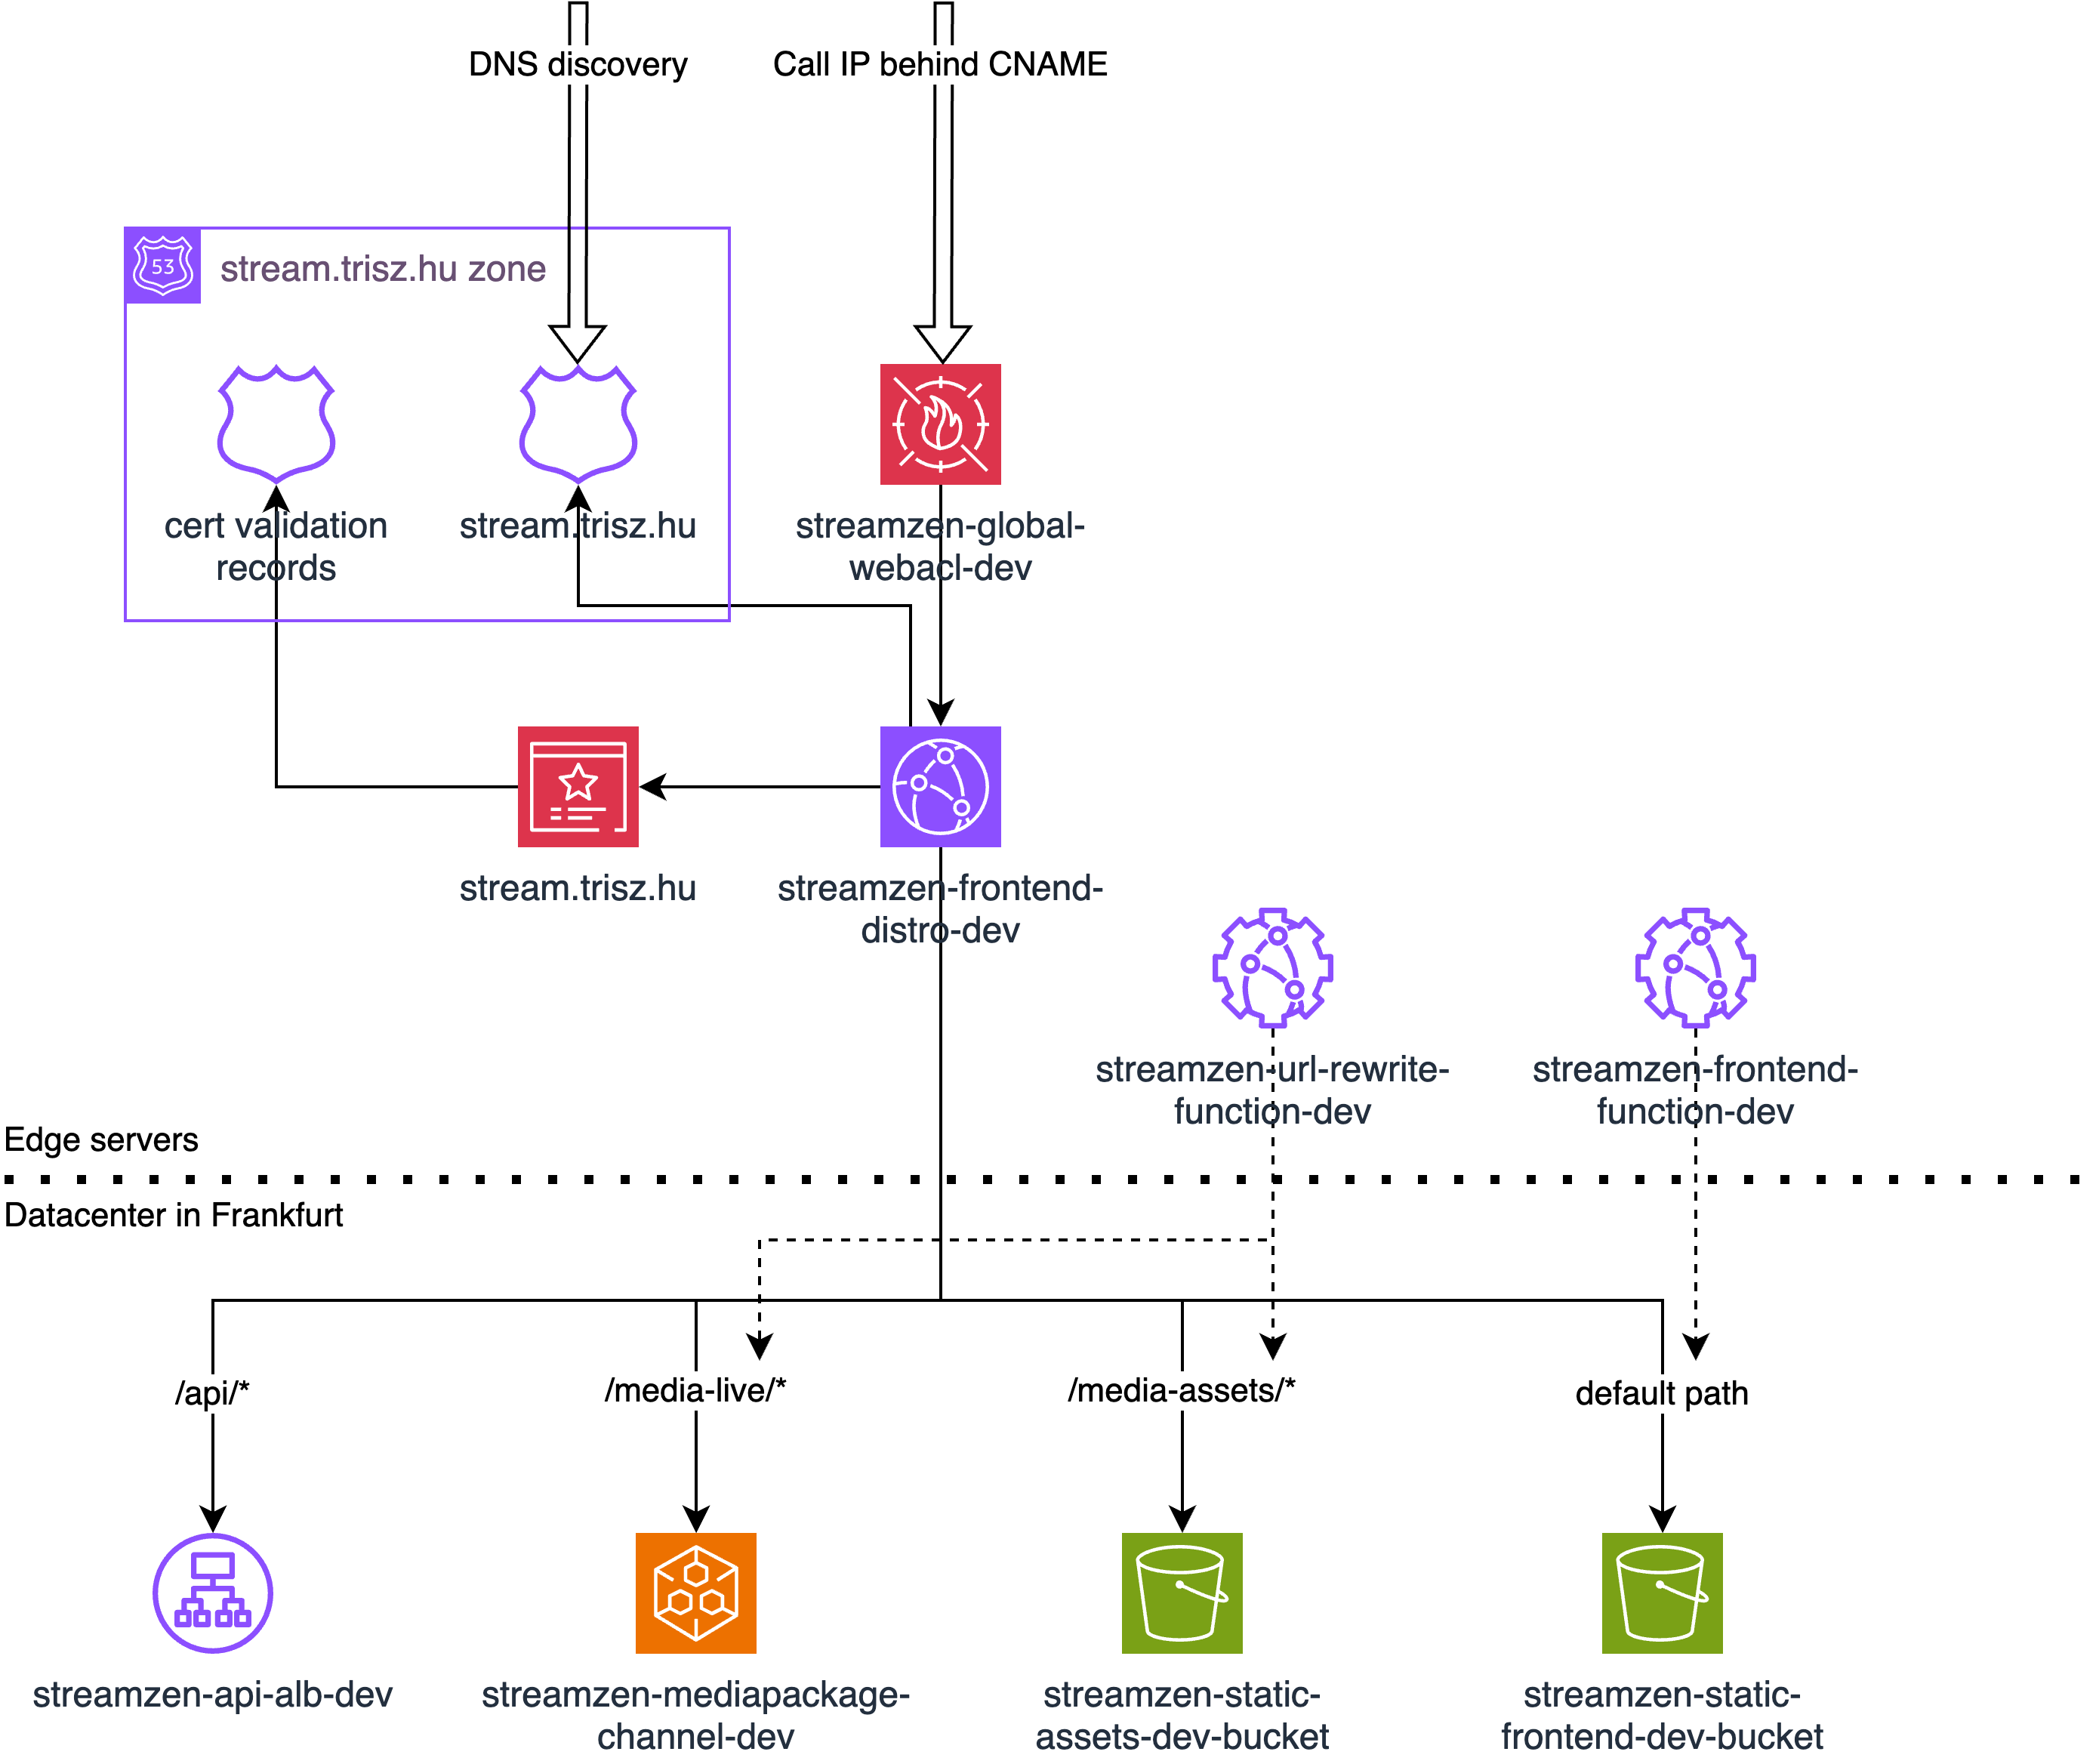
\includegraphics[width=150mm, keepaspectratio]{figures/dipterv_client.png}
  \caption{A kliensoldali architektúra részletesebben.}
  \label{fig:client}
\end{figure}

\Az+\refstruc{fig:client} adatközpont (angolul \emph{datacenter}) felőli oldalán láthatóak a nyilak végén, hogy milyen útvonalak alapján kerül a kérés melyik originhez. A kiértékelés során a disztribúció figyelembe veszi a szabályok sorrendjét, az szabályokban definiált útvonalmintákra mintaillesztés történik, és ha kapott útvonal illeszkedik a sorban következő mintára, ott véget és a kiértékelés. A disztribúcióhoz tartozó originok közül a legfontosabb a statikus weboldal, amely az S3-vödörben található, ez lett az alapértelmezett útvonal, ahova a kérések mennek, amennyiben egyik előbbi útvonalmintára se illeszkedik a kérésben található útvonal.

A CloudFront biztosítja, hogy kis számításigényű logikát tudjuk még az edge rétegében futtatni a kéréseken, erre CloudFront Function-függvényeket alkalmaztam a~MediaPackage-csatorna előtt és a VOD-okat kiszolgáló S3-vödör (\verb|static-assets|) előtt. Ez az \verb|url-rewrite| kis függvény egy \verb|url-rewrite.js| nevű fájlt futtat (\ref{lst:urlrewrite}. kódrészlet). A függvény a kérés URI-ját vizsgálja, és ha a kérés a \verb|/media-assets/| vagy \verb|/media-live/| előtaggal kezdődik, akkor eltávolítja ezeket az előtagokat, és a kérés így megtisztított URI-ját továbbítja a konkrét origin felé.

\begin{minipage}{0.92\textwidth}
  \begin{lstlisting}[
  caption=url-rewrite.js fájl tartalma.,
  label=lst:urlrewrite,
  basicstyle=\fontsize{10}{12}\ttfamily,
  style=js,
]
function handler(event) {
  const request = event.request;
  ["/media-assets/", "/media-live/"].forEach((prefix) => {
    request.uri = request.uri.replace(prefix, "/");
  });
  return request;
}
\end{lstlisting}
\end{minipage}

A backend \verb|/api| előtagú útvonalakon keresztül elérhető, a CloudFront erre egy VPC Origin típusú originként csatlakozik rá, azon keresztül továbbítja a kérést, ezzel leegyszerűsítve a kérések hálózati biztonsági kezelését. Ennek az originnek a cache behaviorje nem igényli, hogy lehagyjuk a \verb|Host| fejlécet, ugyanis az ALB mögötte akár fel tudja használni a forgalomirányításhoz. A többi origin esetén a \verb|Host| fejlécet le kell hagyni a kérésekről (működésük ezt igényli az AWS-dokumentáció alapján dolgozva), ezért is került használatra ezeken az útvonalakon a \verb|Managed-AllViewerExceptHostHeader| nevű Origin Request Policy, azaz ez a kéréseket minden fejléccel együtt továbbítja, kivéve a \verb|Host| fejlécet. A behaviorök mindegyikénél beállítottam, hogyha HTTP-vel jönne a kérés, akkor dobja vissza a kliens felé, hogy kezdje újra HTTPS-en a kérést. A gyorsítótárazási szabályzásokat (angolul \emph{caching}) nem volt célom túlbonyolítani a fejlesztési környezetben, így azt kikapcsoltam. Később ezekkel kísérleteztem (\ref{sec:vod_test}. alfejezet). Az API-n kívül a többinél be kellett állítsam, hogy az alap CORS-fejléceket (\verb|Managed-CORSHeaders|) visszaküldje a kliens felé a disztribúció, hogy a böngésző ne blokkolja a válaszokat. Az API esetében maga a NestJS-alkalmazás kezeli ezt. Ezen beállításokat mutatja be \az+\refstruc{fig:behav} is.

\begin{figure}[h]
  \centering
  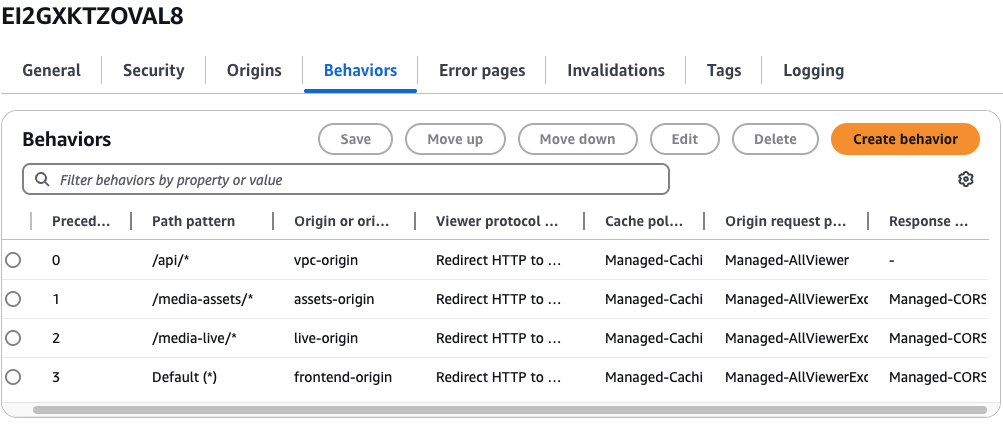
\includegraphics[width=150mm, keepaspectratio]{figures/distro_behav.png}
  \caption{Képernyőkép a különböző útvonalak cache szabályairól.}
  \label{fig:behav}
\end{figure}

A VPC Origin típusú origin a CloudFront-disztribúcióban egy Amazon VPC-n belüli erőforrást jelent -- a mi esetünkben ez az ALB-példányunk --, amelyet a CloudFront közvetlenül elérhet. Nem működik \emph{cross-account} módon, tehát amennyiben a célpont egy másik AWS-fiókban helyezkedne el. Az origin a VPC-n belül található, és elsősorban privát alhálózaton, Security Groupokkal van védve hálózati szinten. A~VPC Origin típusú origin használata lehetővé teszi, hogy a CloudFront közvetlenül kommunikáljon az erőforrással, anélkül hogy nyilvános doménnevet kelljen rendelni hozzá. Ezzel megspórolhatjuk az ALB-példány Internet Gateway-re való kötését, az ALB-példány számára domén bejegyzését, valamint SSL-tanúsítvány felvételét annak, a TLS-kapcsolat is terminálhat a CloudFront-disztribúcióban, házon belül már elég HTTP-alapon forgalmazni komponensek között.

\begin{figure}[h]
  \centering
  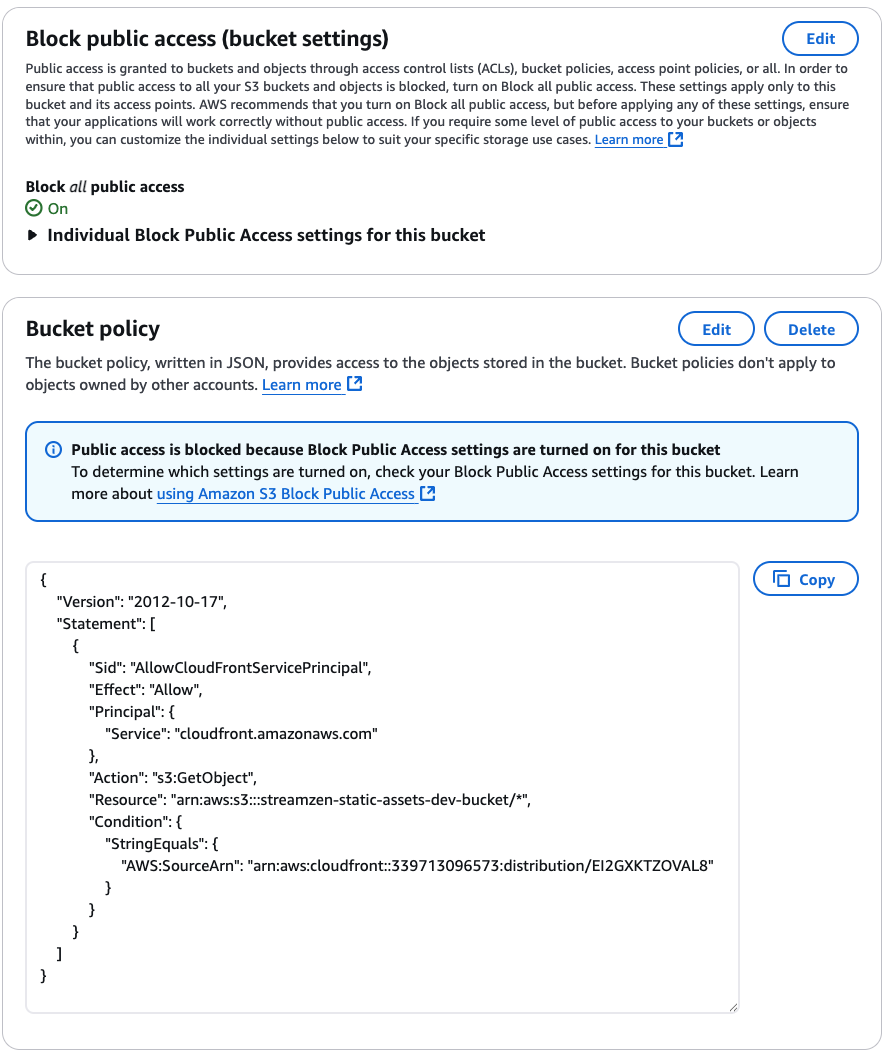
\includegraphics[width=130mm, keepaspectratio]{figures/distro_s3policy.png}
  \caption{Képernyőkép a vödrök hozzáférési beállításairól.}
  \label{fig:s3policy}
\end{figure}

Az S3-vödrök publikus elérését teljes blokkolásra állítottam (\refstruc{fig:s3policy}). Úgy tettem őket elérhetővé a CloudFront-disztribúció számára, hogy egy-egy ``bucket policy''-t csatoltam hozzájuk\cite{s3policy}, amely az S3 originre egyedi, arra csatolt Origin Access Controllal (OAC)\cite{oac} együtt lehetővé teszi, hogy csupán az az AWS-beli principal -- azaz a mi disztribúciónk -- kapjon az objektumolvasásokra (és csak arra) hozzáférést, amelynek a megadott Amazon Resource Number (ARN) azonosítója van. Az ábrán megadott \verb|AWS:SourceArn| a~\verb|streamzen-frontend-distro-dev| disztribúció ARN-je. A fent gyakorolt beállítás is biztosítja az IT-biztonságban is elterjedt és az AWS által is ösztönzött \emph{"principle of least privilege (PoLP)"} elvét.

\begin{figure}[h]
  \centering
  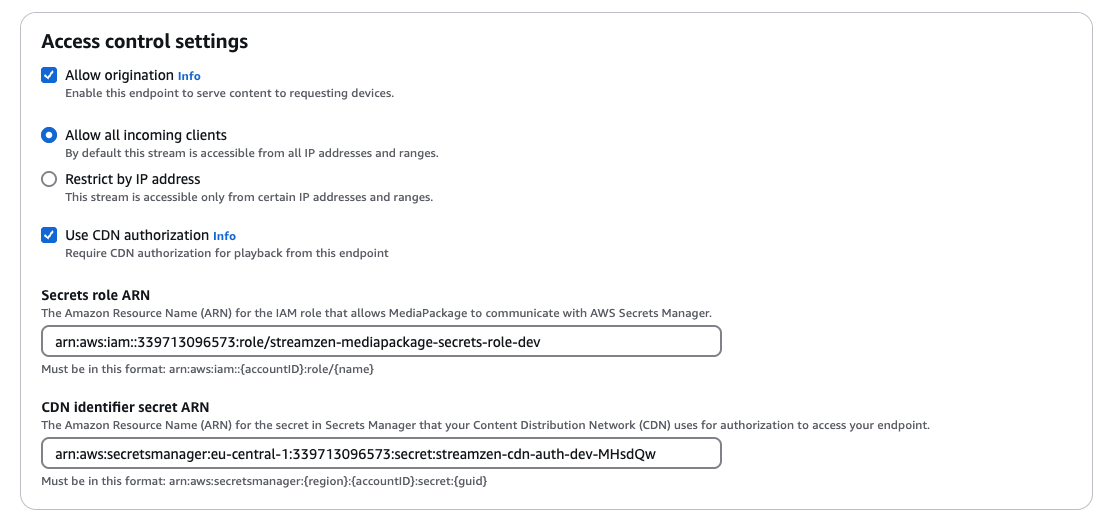
\includegraphics[width=150mm, keepaspectratio]{figures/distro_mediapack.png}
  \caption{Képernyőkép a HLS-végpont hozzáférési beállításairól.}
  \label{fig:mediapack}
\end{figure}

A MediaPackage-csatorna védettségét pedig a publikált HLS-végpontra beállított \emph{CDN Authorization}\cite{cdnauth} segítségével biztosítottam, amely a CloudFront-disztribúciótól érkező kérésekben a \verb|X-MediaPackage-CDNIdentifier| fejlécbe várja el egy titkos kulcs-érték párból az értéket. Ezt a fejlécet a disztribúció felkonfigurálásakor a megfelelő originra rátettem. A MediaPackage-csatorna HLS-végpontjának hozzáférési beállításait, a felhasznált Secret Managerből származó kulcs-érték pár ARN-jét, és az azt elérő IAM-szerep ARN-jét \az+\refstruc{fig:mediapack} mutatja be.

\section{A statikus weboldal}

A statikus weboldal HTML-, JavaScript- és CSS-fájlokból, valamint a weboldal statikus tartalmát képező médiafájlokból (képek, betűtípusok) tevődik össze. Ezek összeállításához a React keretrendszerben írt SPA-alkalmazásokat is jól kezelő Vite.js eszközt használtam, amely a React-alkalmazásokat egyetlen kiindulási \verb|index.html| HTML-fájlba csomagolja, és a készülő JavaScript-kódot is optimalizálja. A Vite.js a fejlesztési környezetben gyorsítótárazza a fájlokat, így gyorsabbá téve a fejlesztést, míg a gyártási környezetben (angolul \emph{in production}) optimalizálja azokat, hogy a lehető legkisebb méretűek legyenek.

Korábban bemutatásra került két különböző CloudFront Function-függvény, amelyek az S3-vödrök elérése előtt futnak minden kérésen. Ezek közül a statikus weboldal előtti függvény (\ref{lst:frontend}. kódrészlet) csupán arra hivatott, hogy a kéréseknél az egyes prefixekkel kezdődő kéréseket átirányítsa az alapértelmezett \verb|/| útvonalra. Ezekre azért volt szükség, hogy a statikus oldal által kezelt útvonalak mind a CDN-re való belépés után az alapértelmezett útvonalon elérhető \verb|index.html|-re oldódjanak fel, hiszen az indexoldalon behivatkozott JavaScriptből pedig majd a betöltés után a React Router megfelelően kezeli le a böngészőben az eredetileg kért útvonalat. Ez a megoldás természetesen magával vonzza azt az igényt, hogy akármikor, ha új aloldalt vezetünk be, akkor a CloudFront Function-függvényben ezt a prefixet hozzá kell adnunk a \verb|routingPrefixes| tömbhöz, amely a kód elején található.

\begin{minipage}{0.92\textwidth}
  \begin{lstlisting}[
  caption=frontend-request-default.js fájl tartalma.,
  label=lst:frontend,
  style=js,
  basicstyle=\fontsize{10}{12}\ttfamily
]
const routingPrefixes = ["/videos", "/live", "/events", "/members", "/courses", "/about", "/studio", "/login"];
function handler(event) {
  const request = event.request;
  if (routingPrefixes.some((pref) => request.uri.startsWith(pref))) {
    request.uri = "/";
  }
  return request;
}
\end{lstlisting}
\end{minipage}

A Vite.js ökoszisztémájának részét képzik különböző fejlesztők által összerakott kódgeneráló szkriptek, a Vite.js hivatalos dokumentációja által ajánlott szkriptek közül választottam a kezdőprojekt felállítására egy olyat, amely TypeScript nyelven írt és React keretrendszerre felkészítve rak össze egy kliensoldali NPM-projektet.

Ezek után telepítettem ebbe a projektbe a könnyebb fejlesztéshez szükséges könyvtárakat, ilyenek például a React Router, a React Hook Forms, az Axios és a Hls.js, utóbbi kettő jelentős szerepet fog még betölteni később implementációs kifejtéseimben. Ezek mellett UI-komponensek kódját húztam be a \emph{shadcn/ui}\footnote{\url{https://ui.shadcn.com/}} könyvtárából, amelyek a felhasználói felület megjelenítéséhez szükségesek.

A Vite.js képes fejlesztői módban indítani egy webszervert arra, hogy folyamatosan figyelje a fájlokat (úgynevezett \emph{watch mode}-ban), és ha változás történik, akkor újrabuildelje a fájlokat, és újraindítsa a webszervert.

\subsection{A weboldal telepítésének CI/CD-folyamata}\label{sec:ciCd}

Előkészítettem egy CI/CD-folyamatot \verb|lint-client.yml| néven a \verb|.github| mappa munkafolyamatai alatt, amely akkor fut le, ha a változtatások giten való feltöltése után készítünk egy Pull Requestet. Ez a munkafolyamat a következő lépéseket hajtja végre: statikus ellenőrzés ESLint\footnote{\url{https://eslint.org/}} használatával, kódformattálás ellenőrzése Prettier\footnote{\url{https://prettier.io/}} használatával, valamint a webalkalmazás lebuildelése. A három lépés hibátlan lefutása jelzi azt, hogy a változtatások után a webalkalmazás telepíthető lesz az S3-vödörbe.

Egy másik folyamat pedig a Pull Request elfogadása és a \verb|main| ágba való beolvasztása után indul el, amely a \verb|deploy-client.yml| néven található. \Az+\ref{lst:deployClient}. kódrészlet mutatja be a kódjának fontos részletét. Két \verb|job| jellemzi a folyamatot, amelyből a második, a konkrét telepítés függ az előző lefutásától, valamint kézzel kell elindítani, amint készen áll (ezt az \verb|environment: production| sor valósítja meg). Az elkészült teljes csomag a Node.js 20-as verziójával buildelődik, majd pedig az elkészült alkalmazás csomagja artifaktként kerül átadásra a következő jobnak. Letöltés után a telepítő szkript az AWS CLI segítségével a~megadott S3-vödörbe tölti fel a fájlokat. A \verb|aws| \verb|s3| \verb|sync| parancs használatával a fájlok feltöltése előtt törli a vödörből azokat a fájlokat, amelyek már nem találhatóak meg a~buildelt fájlok között, így biztosítva azt, hogy mindig csak a legfrissebb fájlok kerüljenek ki a vödörbe.

A GitHub Actionból való AWS-hez való hozzáférést egy külön kompozit akció valósítja meg (\verb|setup-aws| néven), amely az AWS által fenntartott hivatalos ``Configure AWS Credentials'' nevű GitHub Marketplace-en publikált akció\footnote{\url{https://github.com/marketplace/actions/configure-aws-credentials-action-for-github-actions}} v4-es verzióját használja. Ez az akció a megadott AWS IAM-szerepkörhöz tartozó hitelesítő adatokat állítja be a környezeti változókban, amelyeket a következő lépésben használhatunk.

A szerepkör, amelyet a környezet felvesz a \verb|github-oidc-pipeline| névre hallgat. Ezt a szerepkört az infra-bootstrap alprojektből telepítettem korábban az AWS-fiókba. A szerepkört úgy konfiguráltam be, hogy csupán a teljes projektet tároló \verb|streamzen-monorepo| nevű GitHub-repository számára adjon jogosultságot, azaz csak az innen futó GitHub Actionök tudják felvenni a szerepkört. Ez a szerepkör az, amelyet \ref{sec:config} alfejezet is a tervekben bemutatott, amely OIDC nyomán kap hozzáférést.

\begin{minipage}{0.92\textwidth}
  \begin{lstlisting}[
  caption=Részlet a deploy-client.yml fájl tartalmából.,
  label=lst:deployClient,
  style=yaml,
  basicstyle=\fontsize{10}{12}\ttfamily
]
build:
  runs-on: ubuntu-latest
  defaults:
    run:
      working-directory: client
  steps:
    - name: Checkout code
      uses: actions/checkout@v4
    - name: Setup Node.js
      uses: actions/setup-node@v4
      with:
        node-version: 20.x
    - name: Install dependencies
      run: corepack enable && yarn install
    - name: Build
      run: yarn build
    - name: Save bundle
      uses: actions/upload-artifact@v4
      with:
        name: bundle
        path: ./client/dist/
deploy:
  runs-on: ubuntu-latest
  needs: build
  environment: production
  steps:
    - name: Download bundle
      uses: actions/download-artifact@v4
      with:
        name: bundle
        path: /tmp/bundle/dist/
    - name: Setup AWS
      uses: ./.github/actions/setup-aws
    - name: Deploy
      run: aws s3 sync --delete /tmp/bundle/dist s3://streamzen-static-frontend-dev-bucket
\end{lstlisting}
\end{minipage}

\chapter{Szerveroldali folyamatok implementációi}

A megjelenítési réteg alatt található szerveroldali folyamatok implementációja során a~kiszolgáló infrastruktúra kialakítására, a Node.js-alkalmazás fejlesztésére, a konténerizált környezet kialakítására, valamint a videófeldolgozásra fókuszálunk ebben a fejezetben.

\section{A virtuális privát felhő komponensei}\label{sec:vpc}

A szerveroldal erőforrásait igyekeztem mindet egy közös VPC-be szervezni, amely lehetővé teszi, hogy a komponensek egymást lássák, és biztonságosan kommunikáljanak egymással alhálózataik között. A VPC-n belül az összetartozó elemekhez két-két alhálózatot hoztam létre. A legtöbb AWS-szolgáltatás a magas rendelkezésreállás érdekében legalább kettő konkrét adatközpontba kell kitelepítésre kerüljön, azaz az AWS saját terminológiáját használva: két \emph{Availibility Zone}-ba (AZ) kell elhelyezésre kerüljenek a konkrét erőforrások. Ennek megfelelően az eu-central-1 (Frankfurt) régió alatti \emph{eu-central-1a} és \emph{eu-central-1b} AZ-ba szerveztem az egyes alhálózataim. Az alhálózatok közötti forgalom irányítását útválasztó táblák (angolul \emph{route table}) segítségével végeztem, amelyek biztosítják, hogy a~komponensek közötti kommunikáció megfelelően működjön. Az útválasztó táblák konkrét bejegyzéseit, valamint a felhasznált IP-tartományokat is tartalmazza \az+\refstruc{fig:vpc} -- a táblabejegyzések az alhálók jobb felső sarkában egy lila piktogram mellett olvashatóak, a tartományok pedig jobb alsó sarkaikban zöld/kék vastag betűkkel.

\begin{figure}
  \centering
  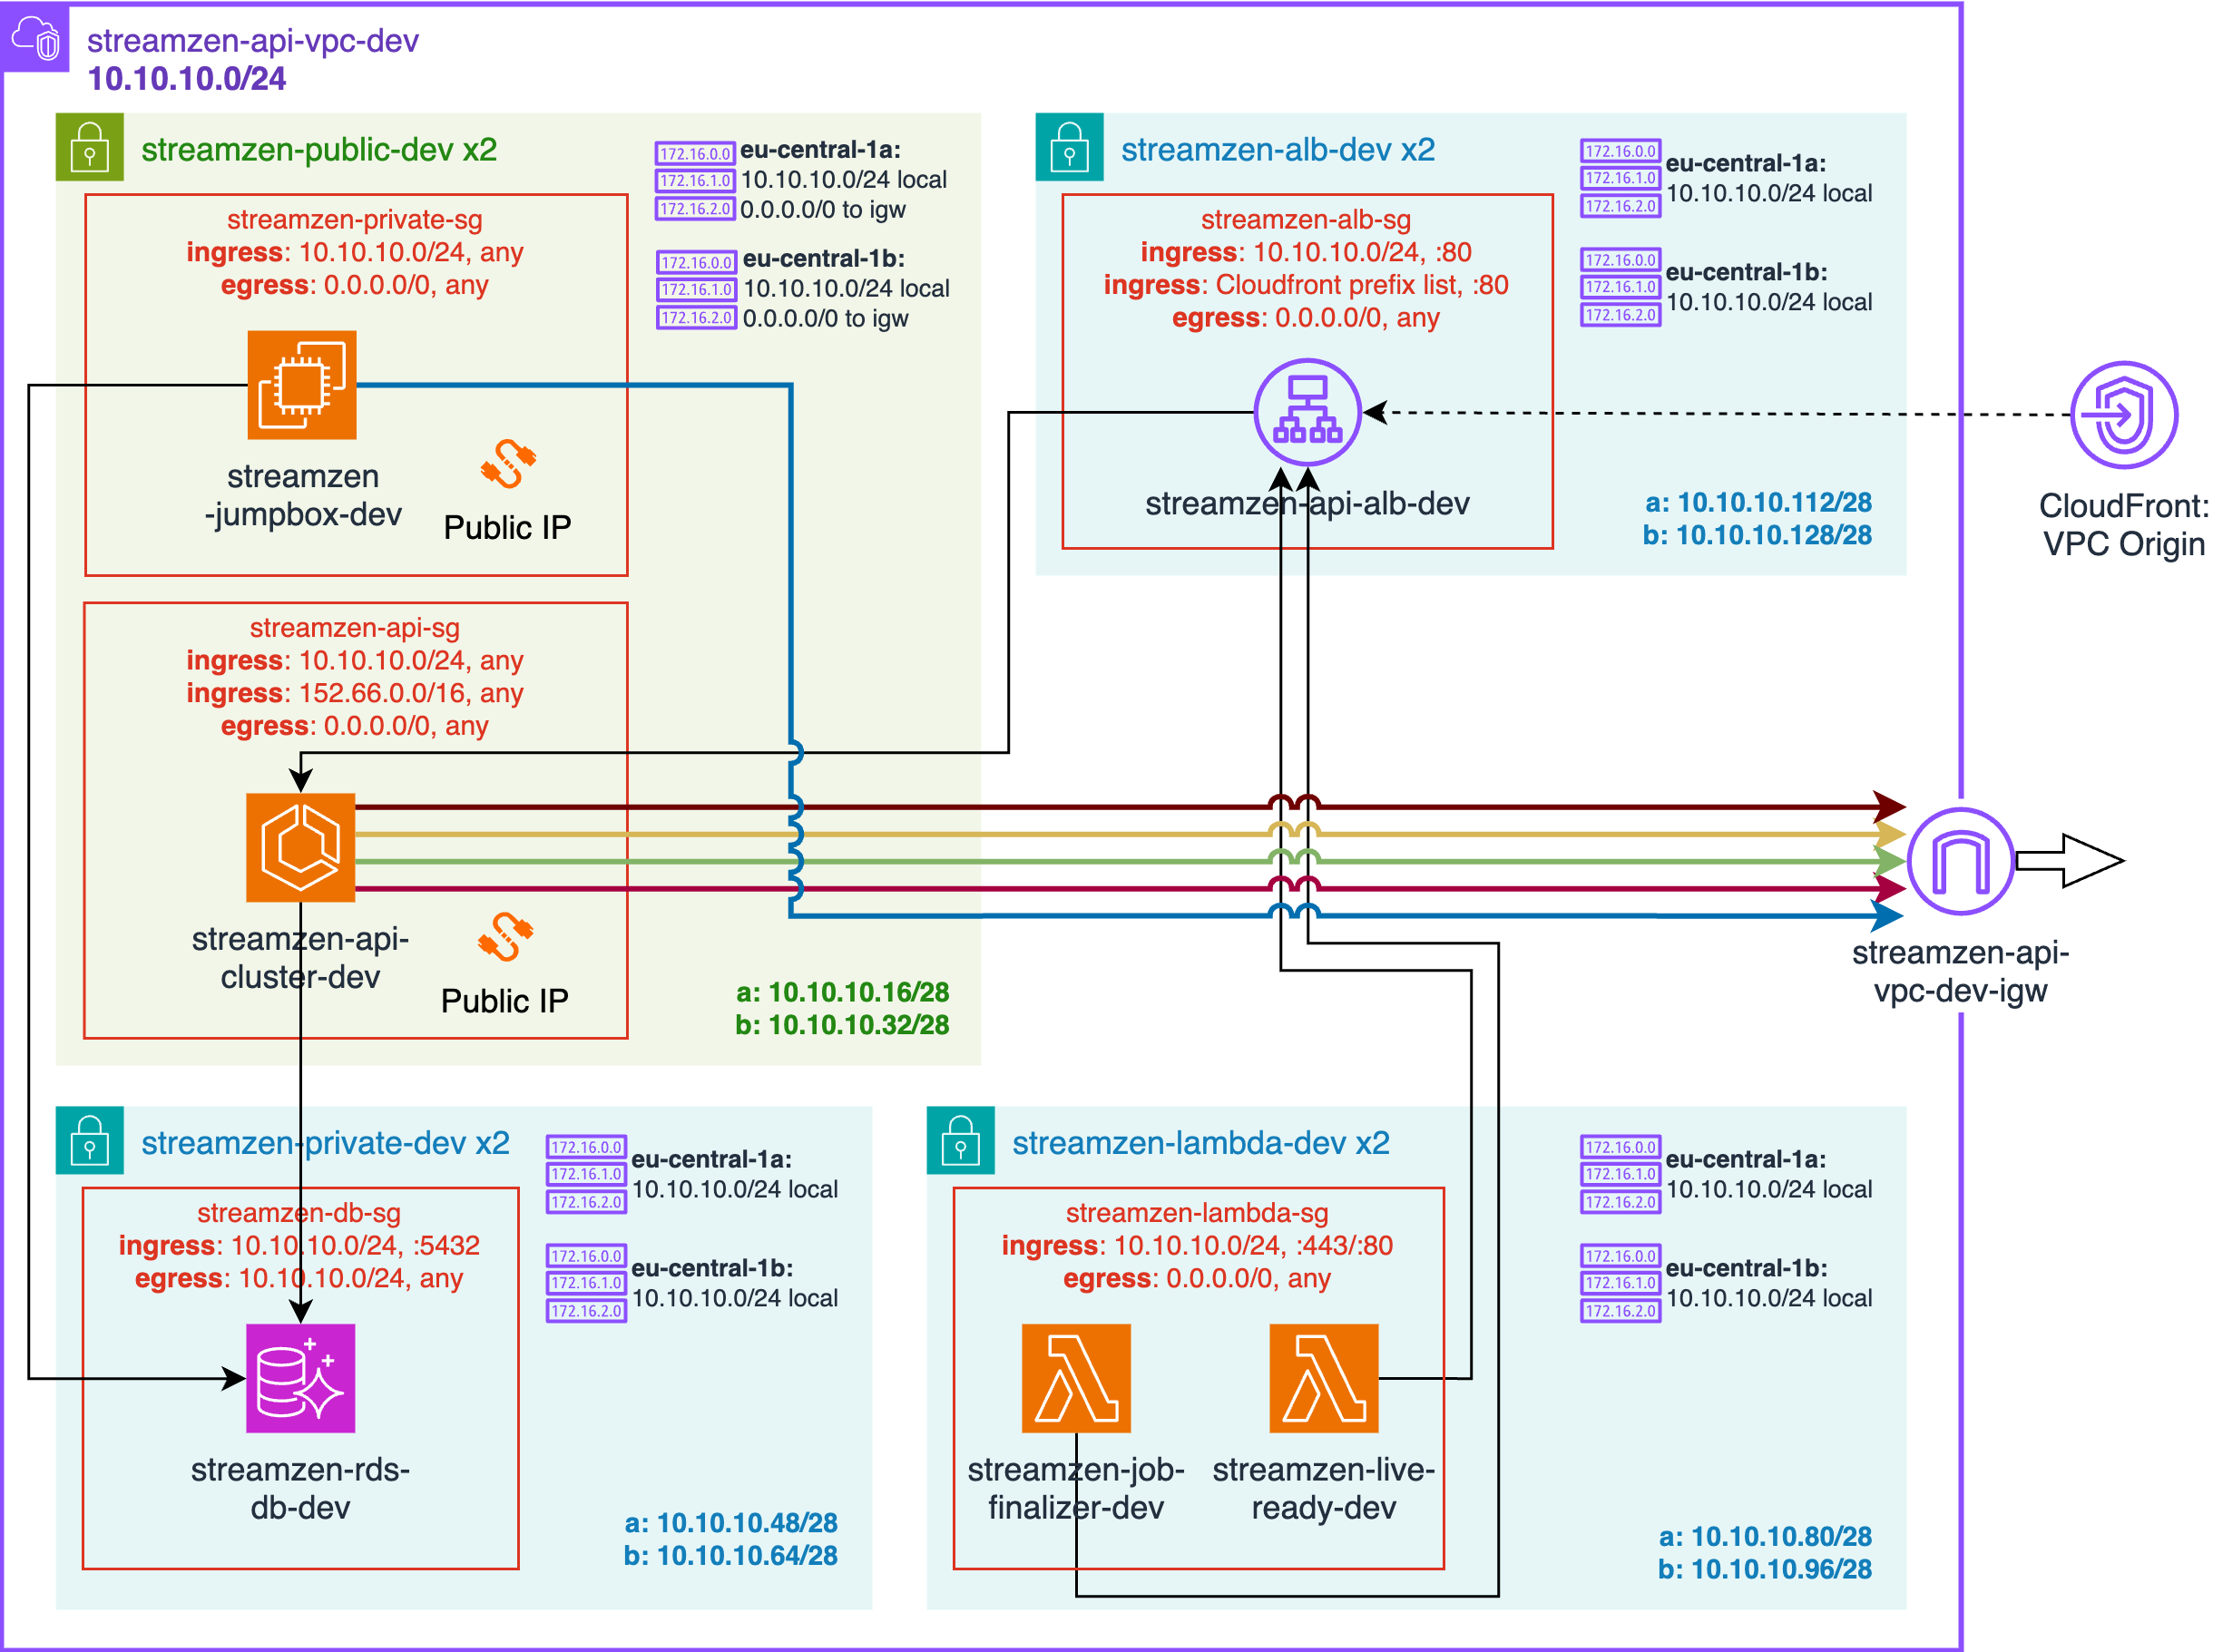
\includegraphics[width=150mm, keepaspectratio]{figures/dipterv_vpc.png}
  \caption{Részletes architektúraábra a VPC-ről.}
  \label{fig:vpc}
\end{figure}

Az ábráról leolvashatóak még a Security Groupok, azaz virtuális állapotmentes tűzfalak, ezek a komponensek vörös keretként látszódnak az ábrán és \verb|-sg| végződésűek neveik. Ezek a tűzfalak úgy kerültek kialakításra, hogy a csupán a ténylegesen szükséges IP-tartományokat és portokat engedélyezzék a kommunikációhoz (\emph{ingress}: bemenő; \emph{egress}: kimenő).

A legelső belépési pontja egy kérésnek az ALB-példány, amely privát alhálózatra lett bekötve. Privátnak minősül egy alhálózat, amennyiben nincs közvetlen internetkapcsolata, nem kerül bekötésre az útválasztó táblájába IGW. Mi esetünkben is csupán az a bejegyzés került be, amely a VPC IP-tartományán belüli kéréseket a VPC-n belül tartja (\emph{10.10.10.0/24 local}).

Habár bevezetésre került egy Internet Gateway (IGW), fontos megjegyezni, hogy nem azért, hogy a kliensoldali erőforrás -- a CloudFront-disztribúció -- elérhesse a szerveroldalt, hiszen azt megvalósítja egy VPC Originen keresztül, amely működési lényege, hogy számára nem szükségeltetik bevezetni publikus alhálózatot, a disztribúció közvetlen összeköttetést tud összehozni VPC-n belül elrejtett hálózati erőforrásokkal, azaz a mi ALB-példányunkkal is\cite{vpcorigin}. Az IGW bevezetésének indokait a következő bekezdések tisztázzák.

Az ECS-klaszter -- amely a Node.js-alkalmazást futtatja és összeköttetésre kerül az~ALB-vel -- publikus alhálózatban helyezkedik el. A Security Groupja úgy lett beállítva, hogy a VPC-n belüli eszközöket engedje be, illetve azt az IP-tartományt, amelyben az AuthSCH is fut (ez a Schönherz Kollégium hálózati tartománya, a 152.66.0.0/16).

A szervernek fontos a kapcsolódása az adatbázisra, amely egy külön privát alhálózatot kapott, abba a Security Group csupán a PostgreSQL-re jellemző 5432 porton keresztül enged és csak a VPC-belülről forgalmat, hasonlóképp kifelé is csak a VPC-n belülre enged.

Az ECS-klaszterben működő szervernek több hálózaton kívül működő szolgáltatás felé kell tudnia kommunikálni. Ezek a VPC-n kívüli komponensek \az+\refstruc{fig:nonvpc} segítségével kerülnek vizuálisan ismertetésre.

\begin{figure}
  \centering
  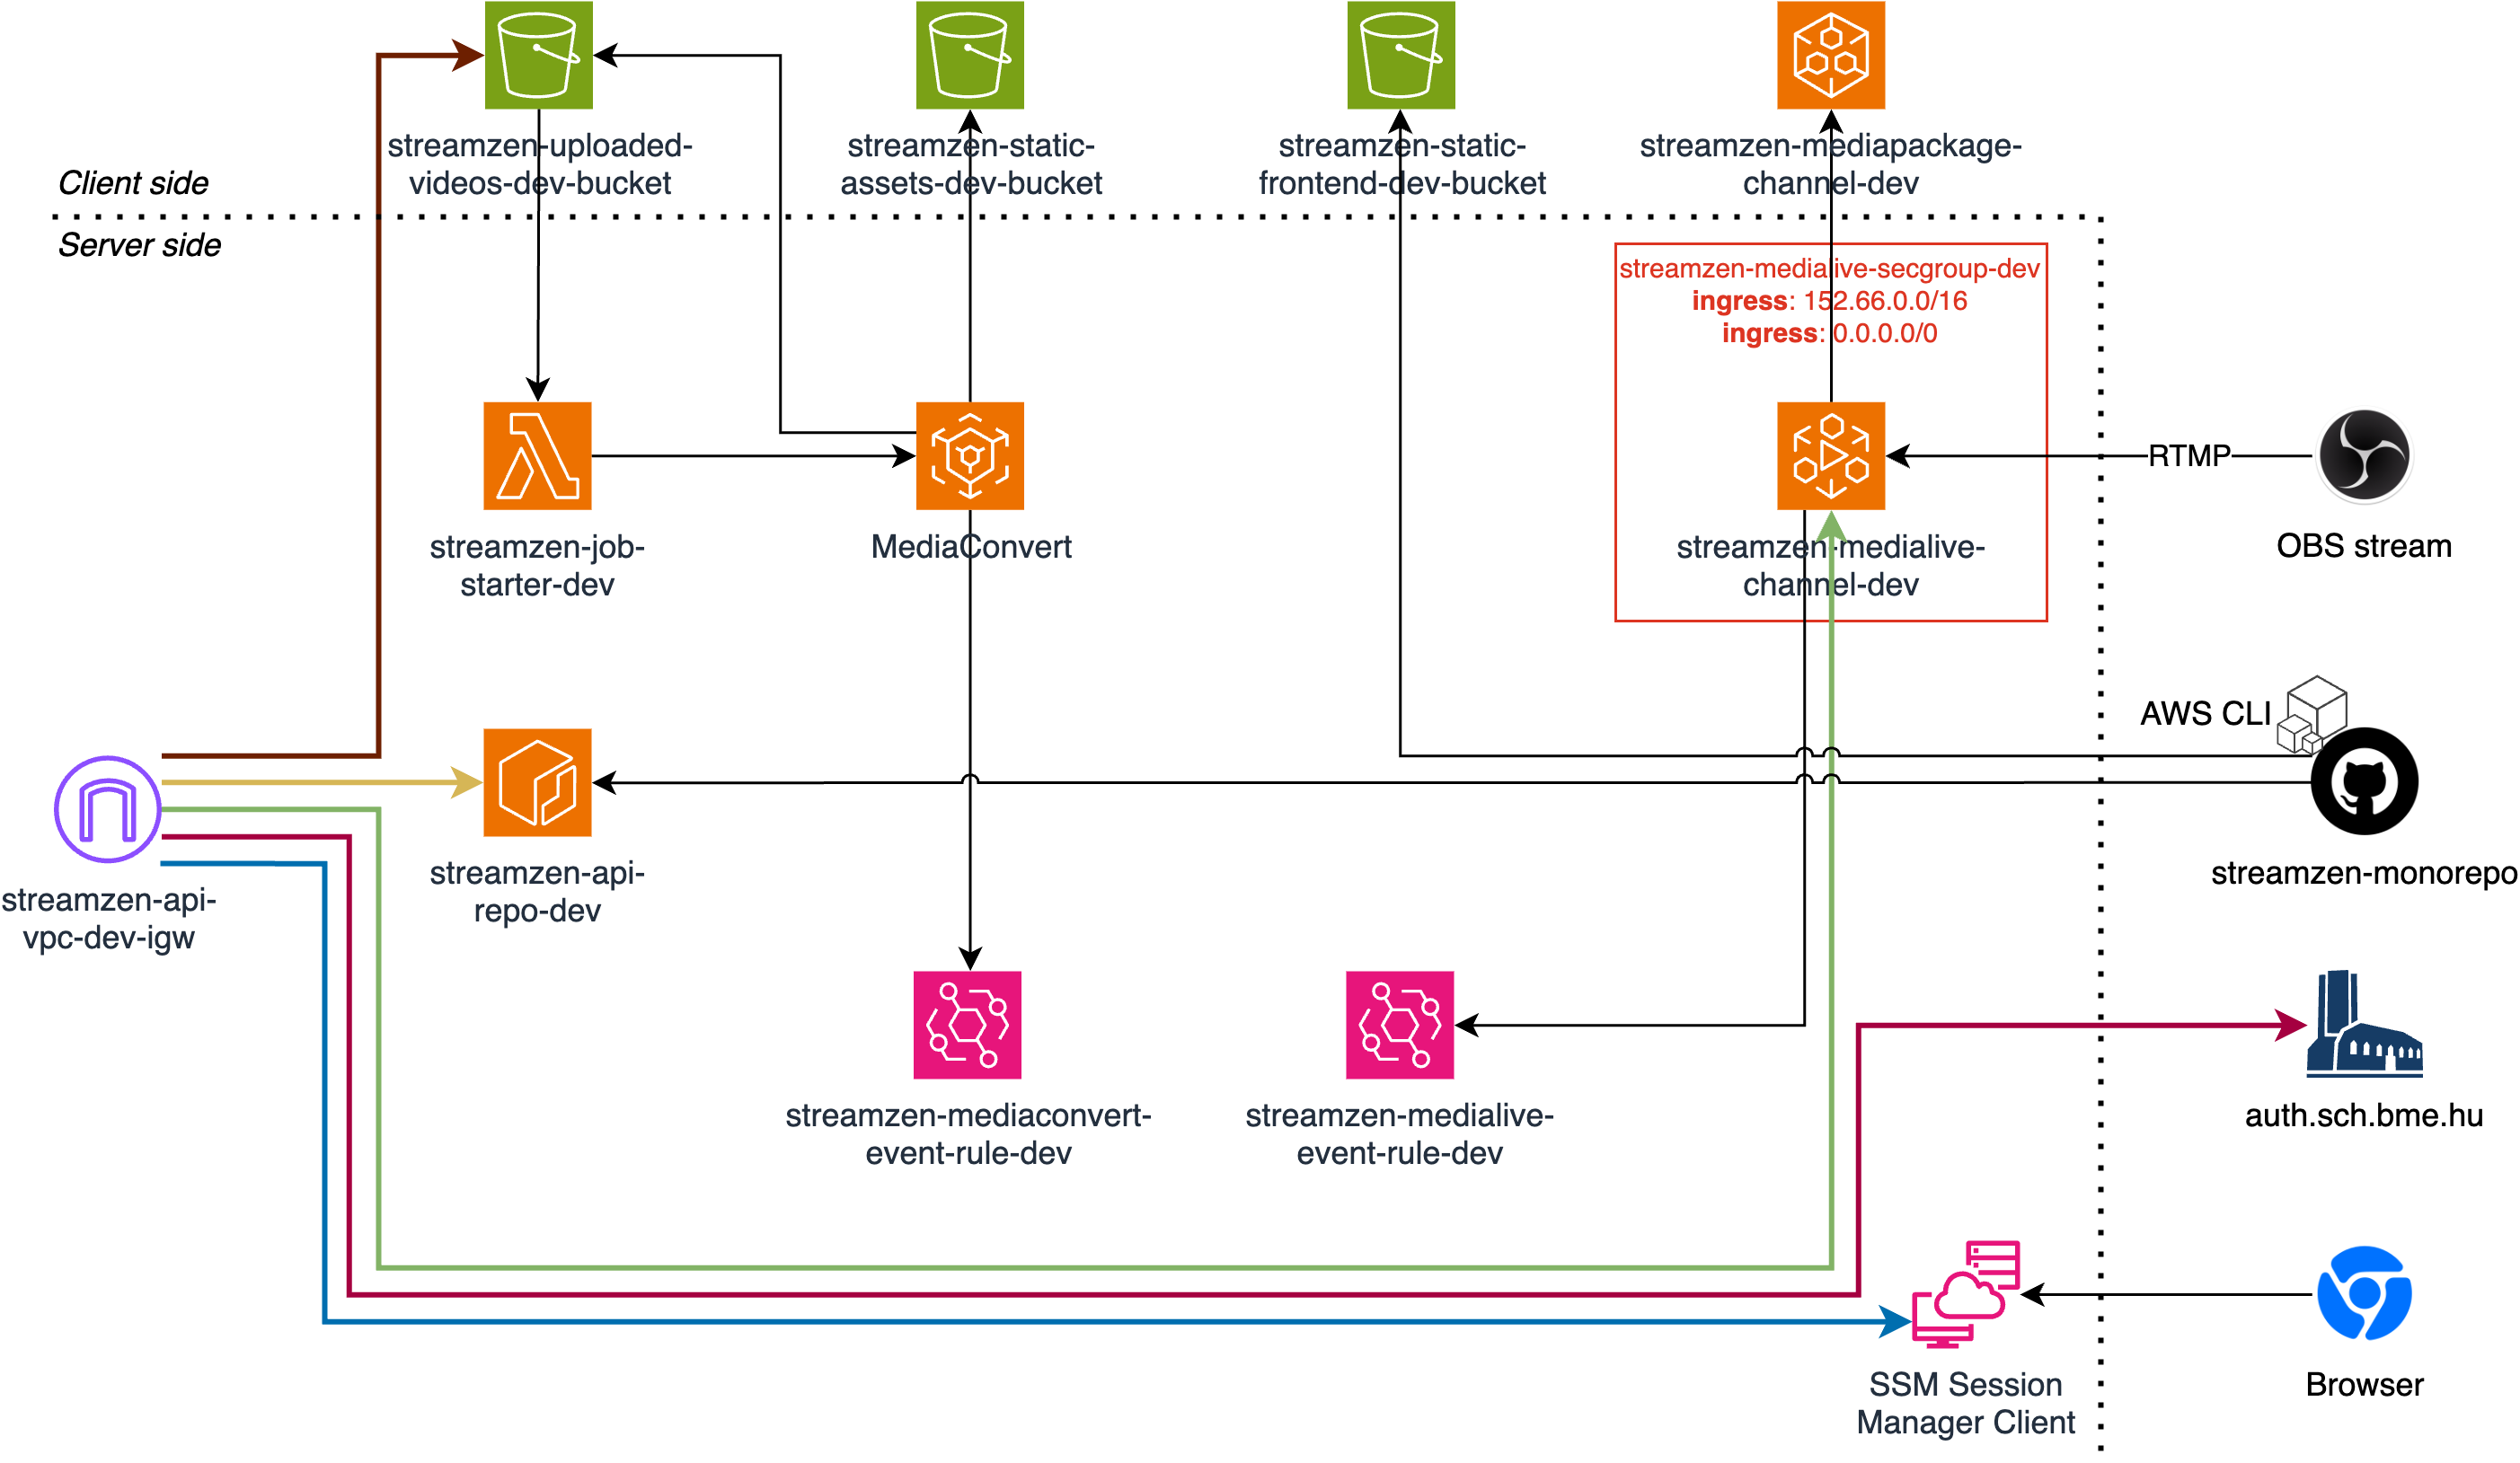
\includegraphics[width=150mm, keepaspectratio]{figures/dipterv_nonvpc.png}
  \caption{Részletes architektúraábra a VPC-ből kifelé és befelé kommunikáló komponensekkel.}
  \label{fig:nonvpc}
\end{figure}

\Az+\refstruc{fig:nonvpc} ábra és \az+\refstruc{fig:vpc} együttesen mutatja be az Internet Gateway-en keresztüli kommunikációs útvonalakat, azonos színű vonalak egyazon kommunikációs útvonalat jelölik. Ennek megfelelően az előző bekezdésben jelölt AuthSCH-t elérő kommunikációs útvonalat követi le a \textcolor{red}{vörös vonal}. A \textcolor{amber}{sárga vonal} jelöli azt, ahogy az ECS-klaszter eléri az~ECR`|tárolót a Docker-kép letöltésére. A \textcolor{green}{zöld vonal} jelöli a szerver és a MediaLive`|csatorna közti utat, amelyen keresztül a szerver elindítja a vételt a csatornán. Végül pedig a \textcolor{brown}{barna vonal} jelöli a videófeltöltés folyamatát az S3-vödörbe a szerveren keresztül.

Léteznek különféle hálózati erőforrástípusok annak kiszolgálására, hogy privát alhálózatban helyezhessünk el egy ECS-ben futó szervert, illetve akár Lambda-függvényeket, amelyeknek kommunikálniuk kell VPC-n kívüli eszközökkel.

Ilyen erőforrástípus a \emph{NAT Gateway}, amely Network Address Translation (NAT) szolgáltatás, és amennyiben adunk neki egy állandó publikus IP-címet (Amazon \emph{Elastic IP} szolgáltatással), úgy képes azon keresztül az internet felé forgalmazást biztosítani a VPC erőforrásai számára, kinti erőforrásoknak viszont befelé már nem. Ez megoldotta volna az AuthSCH felé kommunikálást. Egy másik lehetőség lett volna a~\emph{VPC Endpointok} alkalmazása, amelyek interfészt szolgáltatnak bizonyos AWS-en belüli szolgáltatások felé anélkül, hogy az elhagyná az adatközpontot. A bizonyos szolgáltatások közé tartozik a CloudWatch Logs, az ECR, az ECS-hez tartozó egyéb szolgáltatások, az EventBridge és az S3 is.\cite{vpcEndpoints} Ezt a biztonsági kockázatot a kísérletem szempontjából nem kívántam megelőzni, az igazán szükséges védelmi réteget a Security Group is megvalósítja, a privát alhálózat csupán plusz egy réteget jelent nagy kockázatú, vegyes forgalmat kezelő vállalati rendszerek kivitelezése során, az én esetemben a költségek és a bonyolultság erősen megnőtt volna jelölt erőforrások bekötésével.

A hálózat építése tégláról téglára került kivitelezésre, a fejlesztési/tervezési fázisban ezért érdemesnek tartottam a tesztelés során \emph{``jumpbox''} jelleggel bevezetni egy EC2`|példányt, amely a publikus alhálózatban helyezkedik el. Viszont annak elérésér nem kívántam jelszavakat, SSH-kulcsokat kezelni, ezért az AWS Systems Manager (SSM) Session Manager szolgáltatását használtam, amely lehetővé tette, hogy a webes konzolon keresztül SSH-kapcsolatot létesítsek az EC2-példánnyal anélkül, hogy közvetlenül elérném azt. Az~EC2-es példány létrehozása után egy ágenset kellett volna telepítsek (amihez be kellett volna tudjak lépni közvetlen a gépre), amely erre felkészíti magát a virtuális gépet, azonban ezt a telepítési folyamatot is automatizáltam a Systems Manager Host Management szolgáltatásával, amely lehetővé teszi az EC2-példányok központi kezelését. A jumpbox segítségével tudtam pingelgetni a hálózati eszközök interfészeit, illetve a~Security Groupok beállításait is tesztelni, és akár az RDS-adatbázison is futtatni egyszerű lekéréseket, sémamigrációkat.

\section{A Node.js-alkalmazás fejlesztése}\label{sec:nodejs}

A NestJS keretrendszerben írt Node.js-alkalmazások modulokra bomlanak, az egyes modulok \emph{controller} rétegre és \emph{service} rétegre válnak ketté, a javaslat, hogy az előbbi réteg osztályaiban a forgalomirányítást valósítsuk meg, a későbbiben pedig a konkrét szolgáltatásszintű üzleti logikát, a számításokat, adattisztítást, adatelérést valósítsuk meg. A~modulok implementációjában az egyes \emph{service} és \emph{controller} típusú osztályok példányainak beinjektálását, illetve azok életciklusáról való gondoskodást a NestJS által biztosított Dependency Injection (DI) rendszer valósítja meg.

Az elkészült webszerver-alkalmazás egy REST API-t valósít meg. A benne kialakításra került modulok a következő funkciókat látják el:

\begin{enumerate}
  \item \verb|AuthModule|: A felhasználók azonosításáért és jogosultságkezeléséért felelős modul.
  \item \verb|PrismaModule|: Csupán behúzza a rendszerbe a projektbe telepített Prisma ORM-et mint service.
  \item \verb|UsersModule|: A felhasználók kezeléséért felelős modul, amely a felhasználók CRUD-műveleteit valósítja meg.
  \item \verb|VideoModule|: A videók kezeléséért felelős modul, amely a videók feltöltését és metaadatainak kezelését valósítja meg.
\end{enumerate}

\subsection{Az adatbázisséma}

\Az+\refstruc{fig:prismaliser} mutatja be a Prismában írt Prisma-sémát. A séma tartalmaz jövőbeli felhasználásra szánt elemeket, az egyszerűségre törekszik a séma, csupán a lényeges adatokat tároljuk le.

A \verb|User| entitás reprezentálja a felhasználókat, akik megfelelő \verb|role| attribútumérték esetén feltölteni tudnak a weboldalra. A \verb|role| attribútum típusát enum típusra állítottam, amelynek értékei a \verb|USER| és \verb|ADMIN|. A \verb|User|nek számított attribútuma a \verb|vods| és a~\verb|crewMemberships|.

A \verb|Vod| entitás a feltöltött videók metaadatait reprezentálja. A \verb|Vod| entitásnak meg kell adni létrehozáskor egy \verb|User| kapcsolatot, amely a feltöltő felhasználót reprezentálja. Ezenkívül fontos attribútuma a \verb|state|, amely a videó állapotát reprezentálja. A \verb|state| attribútum enum típusú, lehet értéke \verb|UNPROCESSED| (ez a létrehozáskori érték), lehet \verb|UPLOADED| (amikor feltöltésre került), \verb|PROCESSING| (amikor már a MediaConvert dolgozik az átalakításán), \verb|PROCESSED| (amikor véget ért a MediaConvert-job), vagy pedig \verb|FAILED| (amennyiben hiba történt valamelyik fázisban). Segít a videó állapotának nyomon követésében a~\verb|statePercent| attribútum is, amely a MediaConvert által visszaadott százalékos értéket tárolja le.

A \verb|CrewMembership| entitáshoz tartozó tábla a \verb|Vod| és a \verb|User| entitások közötti illesztő tábla (angolul \emph{join table}), saját attribútumokat tud ehhez a kapcsolathoz hozzáadni, kardinalitás szempontjából egy \verb|CrewMembership|nek csak egy \verb|User|t és csak egy \verb|Vod|ot kell kötnie. Egy \verb|Vod|nak persze több \verb|CrewMembership|je is lehet, ugyanígy \verb|User|nek is. Ez az entitás és a \verb|ViewCounter| -- amely a megtekintések számlálóját lett volna hivatott reprezentálni -- aktívan nem került felhasználásra a fejlesztés során, tervezésben maradt csupán, nem volt esszenciális a végső cél megvalósításához.

\begin{figure}[h]
  \centering
  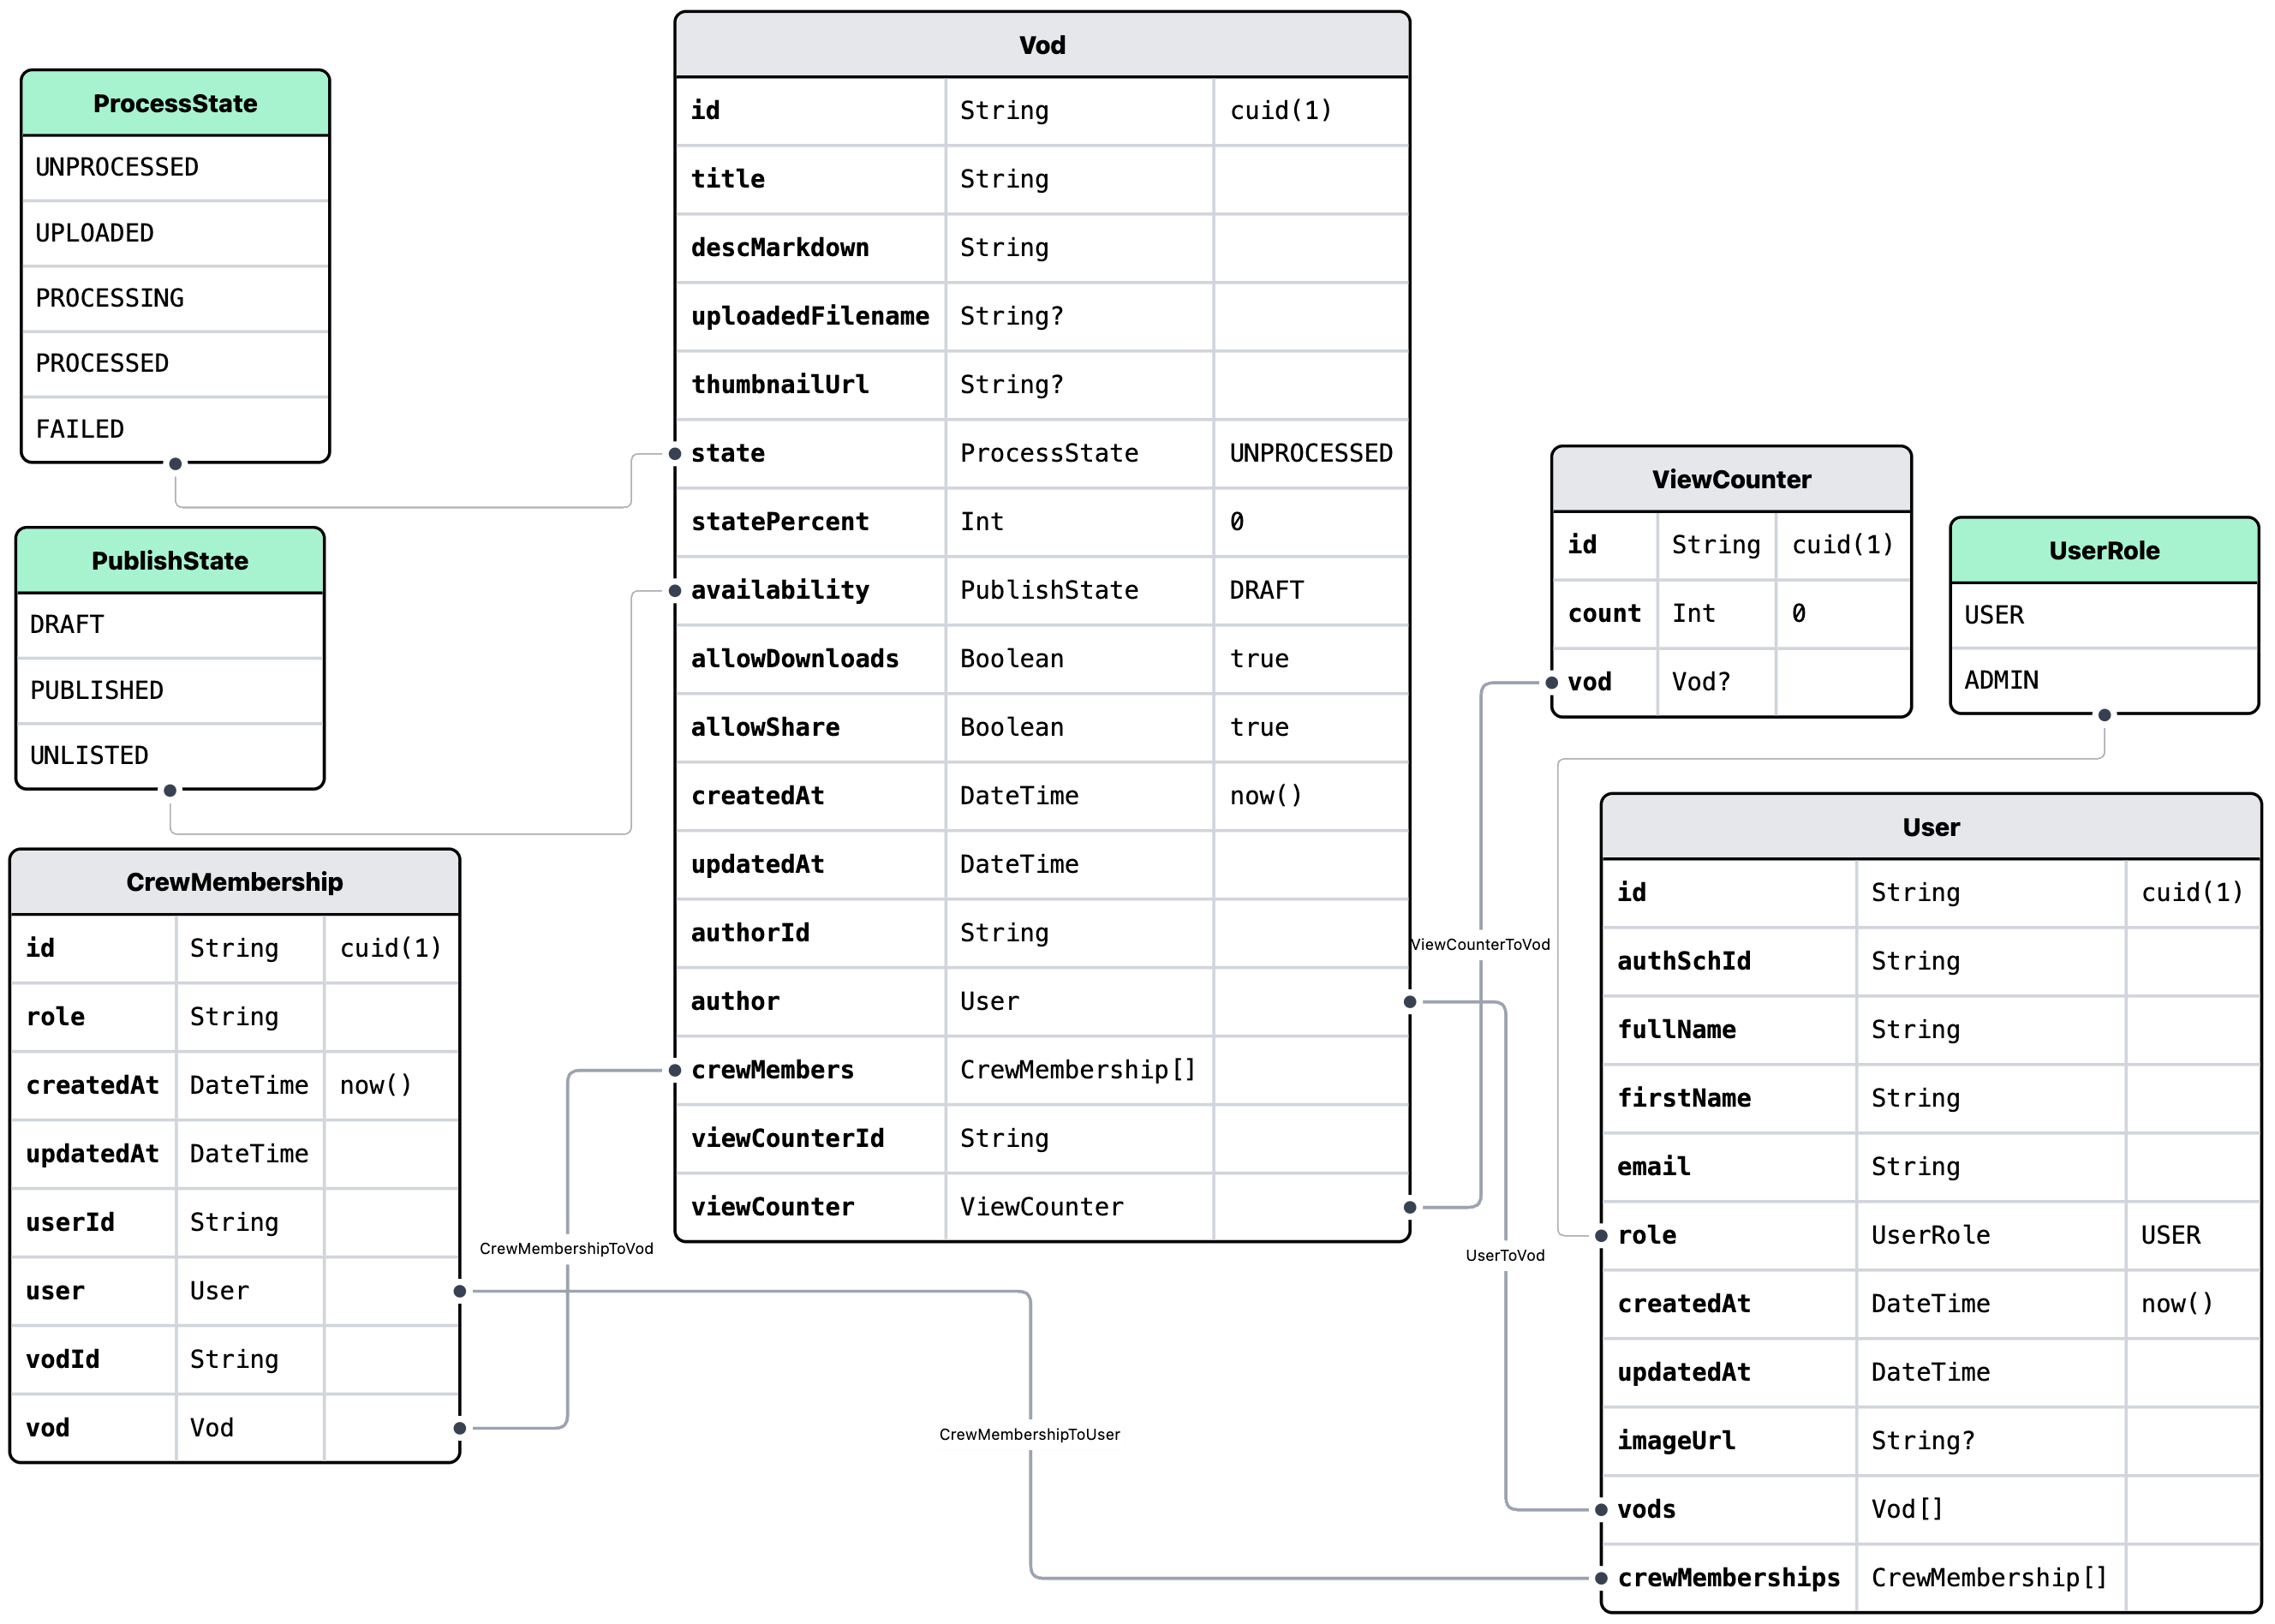
\includegraphics[width=150mm, keepaspectratio]{figures/prismaliser.png}
  \caption{A Prisma-séma vizuális reprezentációja.}
  \label{fig:prismaliser}
\end{figure}

\subsection{Környezeti változók}\label{sec:envvars}

Az alkalmazásnak korábbi alfejezetekben már kiderült, hogy vannak külső függőségei. Ezen függőségekhez való hozzáféréshez a környezeti változók használata elengedhetetlen. Az ECS-ben futó konténer környezeti változóinak beállítására az ECS is ad lehetőséget \az+\ref{lst:mainApi}. kódrészlet mutatja be a Terraform-kód egy részletét, amely átpasszolja az alkalmazás számára a következő fontos paramétereket.

Az AuthSCH SSO-ban felvett OAuth-kliensünk\cite{ietf-oauth-security-topics-13} azonosítóját és titkos kulcsát a~\verb|AUTHSCH_CLIENT_ID| és \verb|AUTHSCH_CLIENT_SECRET| környezeti változók tárolják, ezek értékeit ahogy a kódból is látható egy-egy SSM Parameter Store-ból szerzi meg a CI/CD`|folyamat futtatása során a Terraform-kliensünk (értsd: a referált erőforrás elején \verb|data| kulcsszó jelöli, hogy \emph{data source}-ként éri kéri le a Terraform az AWS CDK-n keresztül az értékét). Ezen Param Store kulcs--érték párokhoz az értéket az AuthSCH saját oldalán szereztem meg \url{auth.sch.bme.hu} oldalon található webes felületén, ahol korábban már megszerzett SCHAcc-fiókomba való belépés után új OAuth-kliens beregisztrálása után tudtam magamnak generálni a kívánt értékeket (ID és client secret).

Egy felhasználónevet és jelszót (\verb|POSTGRES_USER| és \verb|POSTGRES_PASSWORD|) is meg kell tudjuk adni környezeti változón keresztül az alkalmazásunknak, amellyel autentikál az~adatbázisba, ezek értékét is SSM Param Store-okba tettem bele, viszont a felhasználónevet már magam találtam ki, a jelszót pedig magam generáltam kézzel.

Az alkalmazásnak tudnia kell bizonyos átirányítások lekezelésére a kliensünk bázis URL-jét, így azt megadtam környezeti változóban (\verb|FRONTEND_CALLBACK|). A doménnevet változtathatónak véltem hagyni, ezért is került Terraform-változóba az értéke (\verb|var.domain_name|).

Ezenkívül még szükség van egy titkos kulcsra, amely a JWT-tokenek aláírására szolgál (\verb|JWT_SECRET|), ezt is SSM Param Store-ból szerzi be az alkalmazásunk, illetve ezt is már én töltöttem be, miután kézzel generáltam egyet.

A feltöltött videókat tároló S3-vödör nevét (\verb|AWS_S3_UPLOADED_BUCKET|) az általam kitalált nevezéktani konvenciók alapján töltöm be, illetve az S3-vödör régióját (\verb|AWS_S3_REGION|) pedig természetesen arra a régióra állítom, ahová az erőforrások főképp telepítésre kerültek (és ahova az S3-vödör is került).

\begin{minipage}{0.92\textwidth}
  \begin{lstlisting}[
    caption=Az ECS-taszk környezeti változóinak feltöltése Terraformban.,
    label=lst:mainApi,
    style=tf,
    basicstyle=\fontsize{10}{12}\ttfamily,
  ]
task_environment = {
  AUTHSCH_CLIENT_ID = data.aws_ssm_parameter.these["authsch-client-id"].value
  AUTHSCH_CLIENT_SECRET = data.aws_ssm_parameter.these["authsch-client-secret"].value
  POSTGRES_USER = data.aws_ssm_parameter.these["db-username"].value
  POSTGRES_PASSWORD = data.aws_ssm_parameter.these["db-password"].value
  FRONTEND_CALLBACK = "https://${var.domain_name}"
  JWT_SECRET = data.aws_ssm_parameter.these["api-jwt-secret"].value
  AWS_S3_REGION = var.region
  AWS_S3_UPLOADED_BUCKET = "streamzen-uploaded-videos-${var.environment}-bucket"
}
\end{lstlisting}
\end{minipage}

\section{A konténerizált környezet}

A konténerizált webalkalmazás kialakítására a Docker ökoszisztémájának eszközeit vettem alkalmazásba. A fejlesztés során a \emph{Docker Desktop} alkalmazást használtam, amely lehetővé tette a konténerek helyi futtatását, a \emph{Docker Compose} segítségével pedig a~Node.js-alkalmazás mellé felvettem egy PostgreSQL-adatbázis konténerét is, azok között a Compose-kóddal a konténerek közötti kommunikációt is könnyen meg tudtam valósítani.

Az élesítése a Node.js-alkalmazásnak a korábban is ismertetett módon, egy ECS-klaszterba telepítve került kivitelezésre. A szolgáltatás felépítő elemeit, azok működését \az+\refstruc{fig:ecscluster} mutatja be. A felkonfiguráláshoz szükséges Terraform-kódot \az+\ref{lst:ecsCluster}. kódrészlet mutatja be. A klaszterba csupán egy szolgáltatás került be: a REST API-t kiszolgáló webszerver.

\begin{figure}[h]
  \centering
  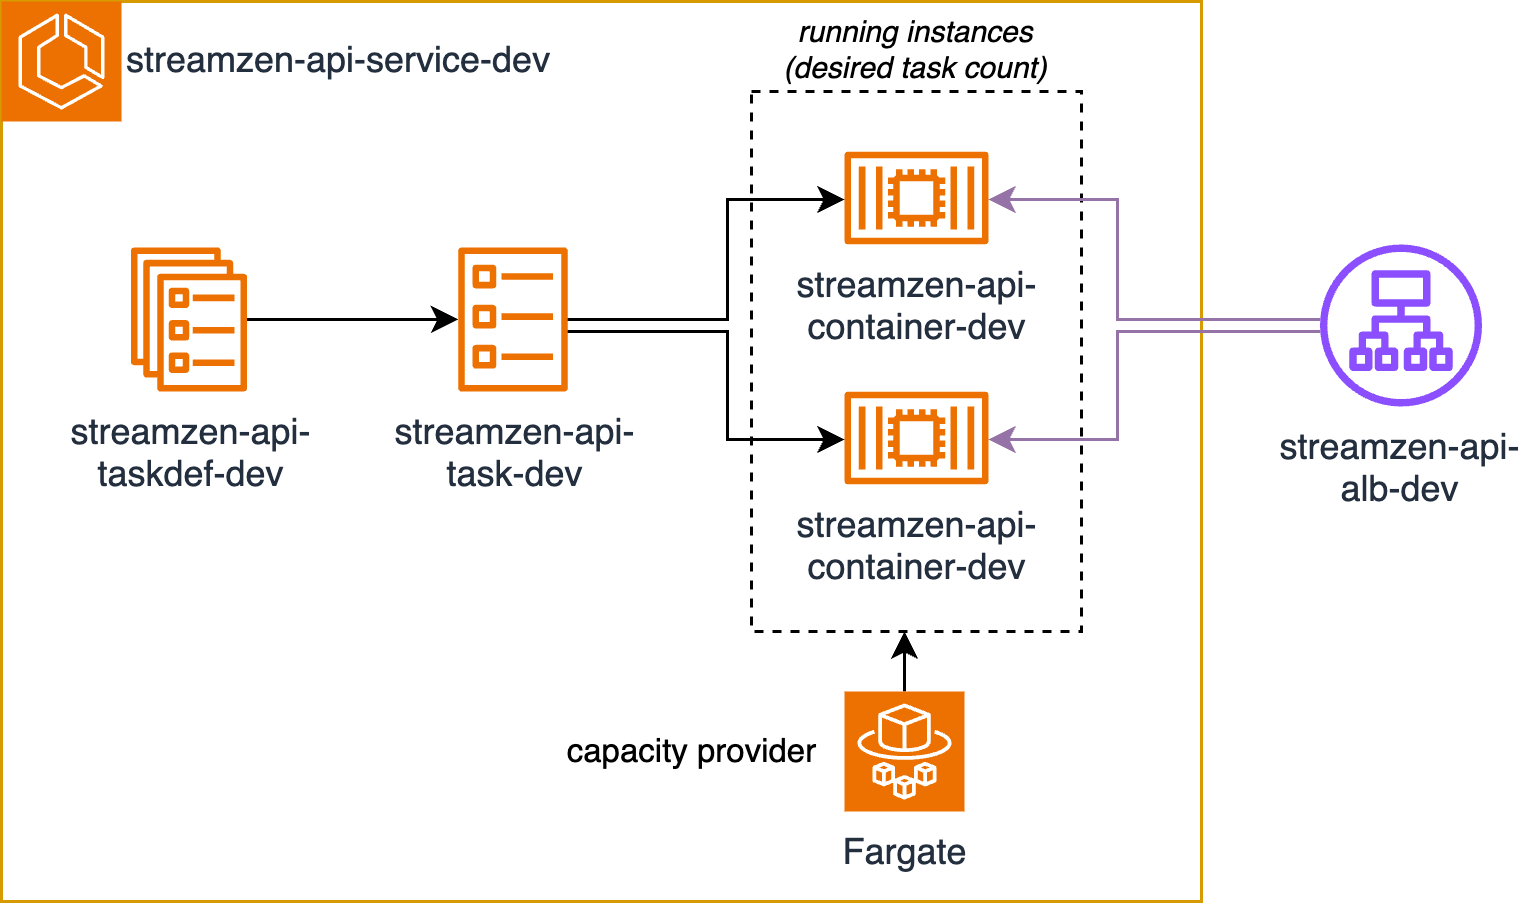
\includegraphics[width=120mm, keepaspectratio]{figures/dipterv_ecs.png}
  \caption{Az ECS-klaszter elemei.}
  \label{fig:ecscluster}
\end{figure}

Egy taszkdefiníciója van a teljes szolgáltatásnak, emiatt egyfajta taszk fog futni is, az fogja kitelepíteni a konkrét konténerpéldányokat. A taszk a konténerek képét természetesen a korábban ismertetett ECR-tárolóból tölti le, majd buildeli le. A konténerek erőforrásmenedzsmentjét a Fargate szolgáltatásra hagytam (lásd: \verb|launch type|). Az ECS-szolgáltatáshoz definiálja kapcsolatát az ALB-példánnyal (lásd: \verb|load balancer| blokk a~Terraform-kódban), az ALB pedig képes automatikusan felderíteni a konkrét konténereket, azokra pedig ráirányítani a forgalmat.

\begin{minipage}{0.92\textwidth}
  \begin{lstlisting}[
    caption=A klaszter és szolgáltatás Terraform-kódja.,
    label=lst:ecsCluster,
    style=tf,
    basicstyle=\fontsize{10}{12}\ttfamily
  ]
resource "aws_ecs_cluster" "this" {
  name = "streamzen-api-cluster-${var.environment}"
}
resource "aws_ecs_service" "this" {
  name            = "streamzen-api-service-${var.environment}"
  cluster         = aws_ecs_cluster.this.arn
  task_definition = aws_ecs_task_definition.this.arn
  desired_count   = var.ecs.desired_task_count
  launch_type     = "FARGATE"

  health_check_grace_period_seconds = 300
  network_configuration {
    subnets          = var.api_subnet_ids
    security_groups  = var.api_secgroup_ids
    assign_public_ip = true # false if you have a NAT GW
  }
  load_balancer {
    target_group_arn = aws_lb_target_group.this.arn
    container_name   = "streamzen-api-${var.environment}"
    container_port   = var.ecs.port_mapping
  }
}
\end{lstlisting}
\end{minipage}

Az ECS egy orkesztrációs környezet is, a segítségével be tudjuk konfigurálni, hogy a konténerek miképp naplózzanak, milyen portokat nyissanak meg, milyen erőforrásokat használjanak, illetve milyen környezeti változókat kapjanak. \Az+\ref{lst:ecsTask}. kódrészlet mutatja be a taszkdefiníciót. A taszkdefinícióban található \verb|container_definitions| blokkban található a konténerre vonatkozó beállítások többsége. Naplózásra az AWS CloudWatch Logs szolgáltatását használja a konténer.

\begin{minipage}{0.92\textwidth}
  \begin{lstlisting}[
    caption=Az ECS-taszk Terraform-kódja.,
    label=lst:ecsTask,
    style=tf,
    basicstyle=\fontsize{10}{12}\ttfamily
  ]
resource "aws_ecs_task_definition" "this" {
  family                = var.ecs.family_name
  container_definitions = jsonencode([{
    volumes          = []
    mountPoints      = []
    healthCheck      = try(var.ecs.health_check, {})
    portMappings     = local.port_mappings
    environment      = [for k, v in var.ecs.task_environment : { name = k, value = v }]
    memory           = var.ecs.memory,
    cpu              = var.ecs.cpu,
    image            = "${aws_ecr_repository.this.repository_url}:latest",
    essential        = true,
    name             = "streamzen-api-${var.environment}",
    logConfiguration = {
      logDriver = "awslogs",
      options   = {
        awslogs-group         = aws_cloudwatch_log_group.this.name
        awslogs-region        = data.aws_region.current.name
        awslogs-stream-prefix = "ecs-streamzen-api-${var.environment}"
      }
    }
  }])
  network_mode             = "awsvpc"
  requires_compatibilities = ["FARGATE"]
  memory                   = var.ecs.memory
  cpu                      = var.ecs.cpu
  execution_role_arn       = aws_iam_role.ecs_service_install.arn
  task_role_arn            = aws_iam_role.ecs_service.arn
}
\end{lstlisting}
\end{minipage}

Az \verb|execution_role_arn| az az IAM-szerepkör, amelyet az ECS-motor fog használni ahhoz, hogy AWS-en belüli hívásokat intézzen a~felhasználó nevében, például a CloudWatch Logs szolgáltatásba való naplózásra vagy az ECR-ről való letöltésére a konténerképnek. A \verb|task_role_arn| pedig az a~szerepkör, amelyet konkrétan a taszk kap meg, a~Node.js-app fogja használni, például az~S3-vödörbe való feltöltéshez.

A szerveralkalmazás kódjának a telepítés szempontjából fontos része a Dockerfile, amely leírja a konténerkép felépítéséhez szükséges lépéseket. Ennek kódját mutatja be \az+\ref{lst:dockerfile}. kódrészlet.

\begin{minipage}{0.92\textwidth}
  \begin{lstlisting}[
  caption=Dockerfile tartalma.,
  label=lst:dockerfile,
  style=dockerfile,
  basicstyle=\fontsize{10}{12}\ttfamily
]
# Stage 1: Build the application
FROM node:20-alpine AS build
ENV NODE_ENV=development
WORKDIR /app
COPY package.json ./
COPY yarn.lock ./
COPY .yarnrc.yml ./
COPY prisma ./prisma/
RUN corepack enable
RUN yarn install
COPY . .
RUN npx prisma generate
RUN yarn build

# Stage 2: Create a lightweight container with the built app
FROM node:20-alpine AS production
ENV NODE_ENV=production
WORKDIR /app
COPY --from=build /app/dist ./dist
COPY --from=build /app/package.json ./package.json
COPY --from=build /app/yarn.lock ./yarn.lock
COPY --from=build /app/.yarnrc.yml ./.yarnrc.yml
COPY --from=build /app/prisma ./prisma
RUN corepack enable
RUN yarn install --immutable
RUN npx prisma generate
CMD ["npm", "run", "start:migrate:prod"]
\end{lstlisting}
\end{minipage}

A Dockerfile két szakaszból áll: az első szakaszban a Node.js-alkalmazás kódbázisának lebuildelése történik csak meg -- standard Node.js-appokra jellemző folyamatot mutat be.

A második szakaszban pedig a buildelt alkalmazás kódja kerül átmásolásra kerül egy újabb Node.js\leavevmode\hbox{-}konténerbe, telepítésre kerülnek az importált NPM-csomagok a~\verb|node_modules|-ba viszont ebben a fázisban a lockfile módosításának lehetősége nélkül. A végén még a Prisma ORM-hez szükséges JavaScript-modulokat is legenerálja. Végül beiktatásra kerül az alapértelmezett parancs, amely a konténer indulásakor a fő folyamatot indítja: ez az \verb|npm| \verb|run| \verb|start:migrate:prod| parancs. Ezt a futtató parancsot a~\verb|package.json| fájlban magam definiáltam, a Prisma ORM által biztosított migrációs eszközt hívja meg (\verb|prisma| \verb|migrate| \verb|deploy|), amely a PostgreSQL-adatbázisunkban sémamigrációt hajt végre, létrehozza a megfelelő táblákat vagy frissíti azok oszlopait, aztán pedig indítja a~Node.js folyamatát (\verb|node| \verb|dist/main|).

\subsection{A szerveralkalmazás CI/CD-folyamatai}

A kliensoldalon is került ismertetésre \ref{sec:ciCd} alfejezetben egy olyan GitHub Actions-alapú CI/CD-munkafolyamat, amely az AWS-fiókba lép be GitHub OIDC-t használva. Azonosképp a szerveroldali konténerkép telepítése a változtatások \verb|main| főágba való olvasztása után az ott ismertetett autentikációs módszerrel kerül feltöltésre AWS-re.

Ennek a folyamatnak az esetében egyszerűbb volt a build- és telepítő folyamatot egybeépíteni, egy job végzi a kettőt. Ennek megfelelően a munkafolyamat miután megszerezte az AWS-fiókhoz hitelesítő adatokat, a következő lépéseket hajtja végre: belép az~ECR-beli Docker Registrybe, majd a Docker-képfájlt buildeli, végül pedig feltölti a saját ECR`|képtárolónkba. \Az+\ref{lst:deployServer}. kódrészlet mutatja be a \verb|deploy-server.yml| fájl releváns részét, amely a kifejtett lépéseket hajtja végre.

A szerveroldali Node.js-kód ellenőrzésére is készült egy CI/CD-folyamat, amely a~\verb|lint-server.yml| fájlban található és Pull Requestek létrehozásakor fut le. Ez a munkafolyamat a kliensoldali ellenőrzéshez hasonlóan az \verb|eslint| és a \verb|prettier| eszközöket használja a kód statikus ellenőrzésére és formázására. A munkafolyamat végén utolsó lépésként pedig az NPM-projekt buildelése van ellenőrzésképp.

\begin{minipage}{0.92\textwidth}
  \begin{lstlisting}[
  caption=Részlet a deploy-server.yml fájl tartalmából.,
  label=lst:deployServer,
  style=yaml,
  basicstyle=\fontsize{10}{12}\ttfamily
]
deploy:
  runs-on: ubuntu-latest
  environment: production
  defaults:
    run:
      working-directory: server
  steps:
    - name: Checkout code
      uses: actions/checkout@v4
    - name: Setup AWS
      uses: ./.github/actions/setup-aws
    - name: Login to ECR
      run: aws ecr get-login-password --region eu-central-1 | docker login --username AWS --password-stdin 339713096573.dkr.ecr.eu-central-1.amazonaws.com
    - name: Build image
      run: docker build -t streamzen-api-repo-dev .
    - name: Tag image
      run: docker tag streamzen-api-repo-dev:latest 339713096573.dkr.ecr.eu-central-1.amazonaws.com/streamzen-api-repo-dev:latest
    - name: Push image
      run: docker push 339713096573.dkr.ecr.eu-central-1.amazonaws.com/streamzen-api-repo-dev:latest
\end{lstlisting}
\end{minipage}

\section{Elemental MediaConvert felhasználása}\label{sec:mediaConvert}

A videófeltöltés és a live indítás mindkettő olyan alfolyamata a rendszernek, amelyeknek implementációja eseményvezérelt architektúrában került kivitelezésre (\emph{event-drive architecture}, EDA\cite{eda}). Ennek az architektúrának egy eleme a Node.js-szerver is, amely a korábbi alfejezetekben került bemutatásra. A feltöltés megtörténik a Node.js REST API-ján keresztül, majd pedig beindul egy másodlagos folyamat, amely a feltöltött fájlok átkonvertálásáért felelős. A feltöltés az S3-vödrön egy \verb|"s3:ObjectCreated"| eseményt generál, amelyet egy Lambda-függvény kap el, a \verb|streamzen-job-starter-dev| (\refstruc{fig:nonvpc}).

A Lambda-függvény célja megkomponálni az konvertáláshoz szükséges job definícióját, amely a feltöltött fájlt átkonvertálja HLS-folyamba helyezhetővé, és az elkészült fájlokat egy S3-vödörbe helyezi el (\verb|streamzen-static-assets-dev-bucket|).

\subsection{A MediaConvert-jobot indító Lambda-függvény}\label{sec:jobStarter}

A függvénynek hat környezeti változót adtam meg, ezek szükségesek a MediaConvert-job felépítésére, a legfontosabbak kerülnek bemutatásra. Az AWS-fiókra egyedileg generálódik egy MediaConvert API HTTP-végpont, és ahhoz, hogy ezt megkapjuk, az AWS CLI-nak kell kiadjuk a következő parancsot: \verb|aws| \verb|mediaconvert| \verb|describe-endpoints|. A kapott URI-t a \verb|MEDIACONVERT_ENDPOINT| környezeti változóban passzolom át. Az~\verb|IAM_ROLE_ARN| az IAM-szerepkör ARN-je, feljogosítja arra a függvényt, hogy CloudWatch-ba naplózzon és az \verb|OUTPUT_BUCKET_URI| és \verb|INPUT_BUCKET_URI| változókban jelölt kimeneti és bemeneti S3-vödrökben tudjon olvasni, létrehozni.

\Az+\ref{lst:jobStarterJs}. kódrészlet mutatja be a Lambda-kód fontos részeit. Az \verb|assembleJobCommand| függvény építi fel a MediaConvert API-ja számára a job paramétereit egy óriási JavaScript`|objektumban. A következőket lehet leszűrni az objektumból:

\begin{itemize}
  \setlength{\itemsep}{1pt}
  \setlength{\parskip}{0pt}
  \setlength{\parsep}{0pt}
  \item \textbf{Kimenetek száma}: 4
        \begin{enumerate}
          \setlength{\itemsep}{1pt}
          \setlength{\parskip}{0pt}
          \setlength{\parsep}{0pt}
          \item Kimenet: 1080p képmagasság, max. videóbitráta 10 Mbps, hangbitráta 256 kbps
          \item Kimenet: 720p képmagasság, max. videóbitráta 5 Mbps, hangbitráta 192 kbps
          \item Kimenet: 480p képmagasság, max. videóbitráta 2 Mbps, hangbitráta 128 kbps
          \item Kimenet: 360p képmagasság, max. videóbitráta 1 Mbps, hangbitráta 96 kbps
        \end{enumerate}
  \item \textbf{Kimenetekre azonos mozgóképtulajdonságok}: HLS formátum, H.264 kódolású, 6 másodperces szegmensek, \emph{Quality-Defined Variable Bitrate} (QVBR) bitráta\cite{qvbr}.
  \item \textbf{Kimenetekre azonos hangtulajdonságok}: AAC audiókódolás, konstans bitráta (CBR), 48 kHz mintavételezés, 2 csatorna.
\end{itemize}

Minden más adat/konténertulajdonság, amit nem közöltem, az az alapértelmezett maradt vagy öröklődik a forrás videófájlból.

\begin{minipage}{0.92\textwidth}
  \begin{lstlisting}[
    caption=Részlet a job-starter függvény JavaScript-kódjából.,
    label=lst:jobStarterJs,
    style=js,
    basicstyle=\fontsize{10}{12}\ttfamily
  ]
const assembleJobCommand = (config) => ({
  Queue: config.jobQueueArn,
  UserMetadata: {
    id: `${config.id}`,
    uploadedFilename: `${config.uploadedFilename}`,
  },
  Role: config.iamRoleArn,
  StatusUpdateInterval: "SECONDS_20",
  Settings: {
    OutputGroups: [{
        Outputs: [
          { ... }, // 1080p settings
          { ... }, // 720p settings
          { ... }, // 480p settings
          { ... }, // 360p settings
        ],
        OutputGroupSettings: {
          Type: "HLS_GROUP_SETTINGS",
          HlsGroupSettings: {
            SegmentLength: config.segmentLength, 
            Destination: `${config.dest}`, ...
          },
        }, ...
    }],
    Inputs: [{ FileInput: `${config.origin}`, ... }],
  },
});

export const handler = async (event, context) => {
  const callerInput = event.Records[0].s3;

  const config = {
    jobQueueArn: process.env.JOB_QUEUE_ARN,
    iamRoleArn: process.env.IAM_ROLE_ARN,
    origin: `${process.env.INPUT_BUCKET_URI}/${callerInput.object.key}`,
    dest: `${process.env.OUTPUT_BUCKET_URI}/${callerInput.object.key}`,
    id: callerInput.object.key.split("/")[0],
    uploadedFilename: callerInput.object.key.split("/")[1],
    segmentLength: process.env.SEGMENT_LENGTH ?? 6,
  };

  const data = await emcClient.send(
    new CreateJobCommand(assembleJobCommand(config))
  );
};
\end{lstlisting}
\end{minipage}

\begin{figure}
  \centering
  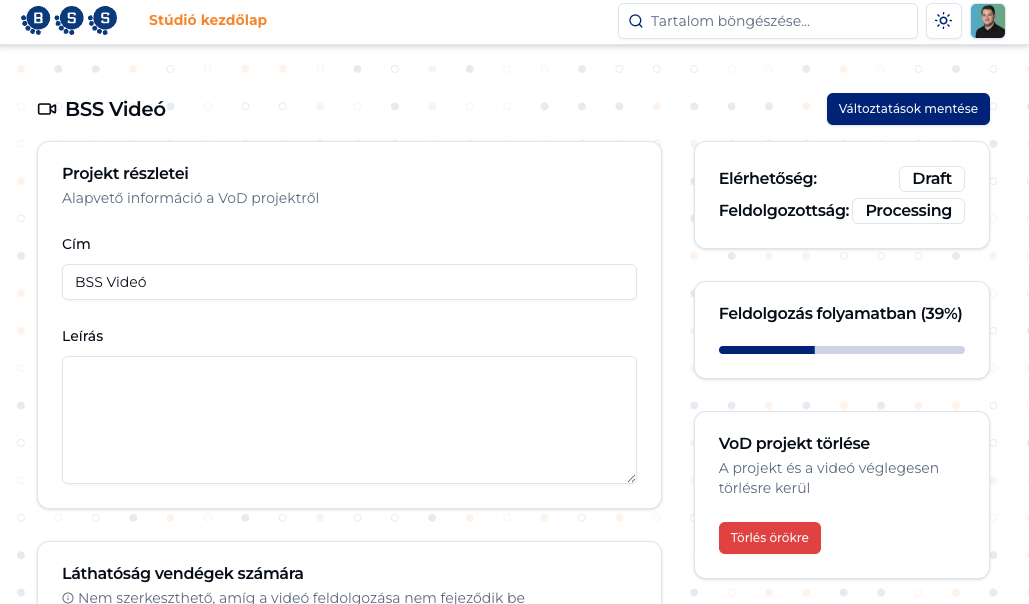
\includegraphics[width=150mm, keepaspectratio]{figures/processing.png}
  \caption{Képernyőkép egy videóprojekt szerkesztői nézetében.}
  \label{fig:processing}
\end{figure}

\Az+\refstruc{fig:processing} bemutatja, miképp kerül visszajelzésre a felületen az, hogy hol áll a feldolgozottsága egy feltöltött videónak. A képernyőképen jelzett ``BSS Videó'' nevű projektbe egy 91 MB-os 1 perc 43 másodperc hosszú videófájl került feltöltésre. A feldolgozást megvizsgáltam a MediaConvert konzoljáról, a job 42 másodpercig tartott. A feltöltött videó további paraméterei ezek voltak:

\begin{itemize}
  \setlength{\itemsep}{1pt}
  \setlength{\parskip}{0pt}
  \setlength{\parsep}{0pt}
  \item \textbf{Mozgóképanyag}: H.264 kódolású, 1920x1080p felbontás, 7 Mbps átlagos bitráta
  \item \textbf{Hanganyag}: AAC kódolás, 256 kbps bitráta, 2 csatorna, 48 kHz mintavételezés
\end{itemize}

\begin{figure}[h]
  \centering
  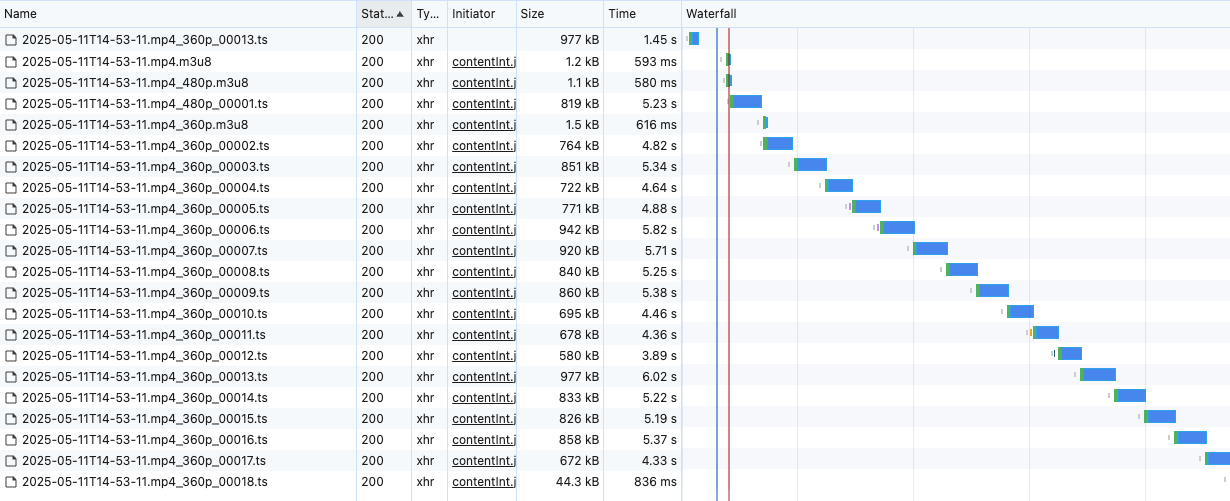
\includegraphics[width=150mm, keepaspectratio]{figures/browser_slow4g.png}
  \caption{Képernyőkép a HTTP-packetek érkezéséről (Slow 4G).}
  \label{fig:slow4g}
\end{figure}

\Az+\refstruc{fig:slow4g} mutatja be, ha átnavigálunk a weboldalon a streamelhető videó oldalára, akkor a böngészőben milyen packetek kerültek letöltésre a videófolyamokból. A böngészőben beállítottam sávszélkorlátozást (\emph{Slow 4G}), és azt tapasztaltam, hogy a böngésző elkezdi a 480p-s folyamot letölteni, majd az első packet után 360p-sre vált. A videót az~első packet megérkezése után rögtön elindítottam, a 360p-s videófolyam bufferelés nélkül tudott lejátszódni.

Kipróbáltam a 3G-s beállítást is a Chrome böngészőben, azon a sávszélen már erősen hosszú bufferelésre volt szükség még a legalacsonyabb 360p-s felbontásnál is. Vártam másfél percet, hogy betöltsön néhány packetet előre a böngésző, utána már simább volt az élmény. Ez jelentős élményromlást tud jelenteni, ha egy körülbelül 2 perces videó lejátszásához is muszáj megállnom és bevárni pár packetet. Igény merülhet fel újabb és spórolósabb kimenetek bevezetésére a konvertálás folyamatába.
A 360p-s packetek átlagban 1,2 MB-osak lettek, a CDN a legtöbbet átlagban 800 kB-osra tudta letömöríteni még. Az 1080p-s packetek átlagban 10 MB-osak lettek, a 720p-sek 6 MB-osak, a 480p-sek 2,4 MB-osak. Ezek esetében is a CDN 30-40\% körüli tömörítést tudott elérni.

\subsection{A MediaConvert-job státuszváltozásának kezelése}

\Az+\ref{lst:emcEventRule}. kódrészlet mutatja be a MediaConvertben futó job eseményeire való feliratkozást. A~\verb|job-finalizer| modulbeli Lambda-függvény roppant egyszerű kóddal rendelkezik, csupán behív az eseményből kapott paraméterekkel (job ID és feldolgozottság százaléka) az~ALB-n keresztül a Node.js-appba a \verb|/api/videos/:id/progress| végponton, a webszerver pedig frissíti az adatbázisban a videó állapotát.

\begin{minipage}{0.92\textwidth}
  \begin{lstlisting}[
    caption=A streamzen-mediaconvert-event-rule-dev Terraform-kódja.,
    label=lst:emcEventRule,
    style=tf,
    basicstyle=\fontsize{10}{12}\ttfamily
  ]
resource "aws_cloudwatch_event_rule" "this" {
  name        = "streamzen-mediaconvert-event-rule-${var.environment}"
  description = "Capture MediaConvert job state changes"
  event_pattern = jsonencode({
    source      = ["aws.mediaconvert"],
    detail-type = ["MediaConvert Job State Change"]
    detail      = {
      status = ["COMPLETE", "ERROR", "STATUS_UPDATE"]
      userMetadata = {
        application = ["streamzen-${var.environment}"]
      }
    }
  })
}

resource "aws_cloudwatch_event_target" "this" {
  rule      = aws_cloudwatch_event_rule.this.name
  target_id = "streamzen-mediaconvert-event-target-${var.environment}"
  arn       = module.job_finalizer.arn
}
\end{lstlisting}
\end{minipage}

\section{A MediaLive és MediaPackage összekötése}\label{sec:mediaLive}

A MediaLive szolgáltatásban fellőttem a tervezett egyetlen csatornát, amelyre egy RTMP push alapú inputot kötöttem be. A létrehozott inputhoz az AWS rendelt IP-t, portot, a~kapott URL így ez lett: \url{rtmp://3.73.170.41:1935/streamzen-dev}. A csatorna úgy lett felkonfigurálva, hogy maximum 20 Mbps bitráta mellett 1080p-s felbontású videófolyamot tudjon fogadni, a hangot pedig AAC kódolásúként, 256 kbps bitrátával. A~MediaLive`|csatornából átvezetett folyam két kimenetet képez, egy 8 Mbps célbitrátájú 1080p-s kimenetet ad, illetve egy 3,3 Mbps célbitrátájú 720p-s kimenetet. A MediaPackage szolgáltatásban is egyetlen csatornát hoztam létre, amely a MediaLive-csatorna kimeneteit fogadja be, és az átkonvertálja HLS-formátumú folyamra.

A MediaLive-csatornának még szüksége volt egy IAM-szerepkörre, amelyben megadtam a szerepkörnek minden olyan jogosultságot, amely szükséges a MediaPackage`|csatornába való átvezetéshez számára, illetve a CloudWatch-ba való naplózásra és a szükséges hálózati/EC2-hez kapcsolódó jogokat is megkapta (a MediaLive hátterében menedzselt EC2-példányok futnak).

A MediaLive-csatorna indítása után lehetséges az input URL-re felcsatlakozva kezdeni a streamelést. Az RTMP streameléshez az OBS Studio nevű alkalmazást használtam\cite{obsMediaLive}, abban a beállításoknál a ``Stream'' menüben kitöltöttem az egyedi RTMP-szerverem adataival a mezőket (lásd \refstruc{fig:obs}). Nem került felhasználásra egyelőre a kísérlet alatt autentikáció a végpontra.

\begin{figure}[ht]
  \centering
  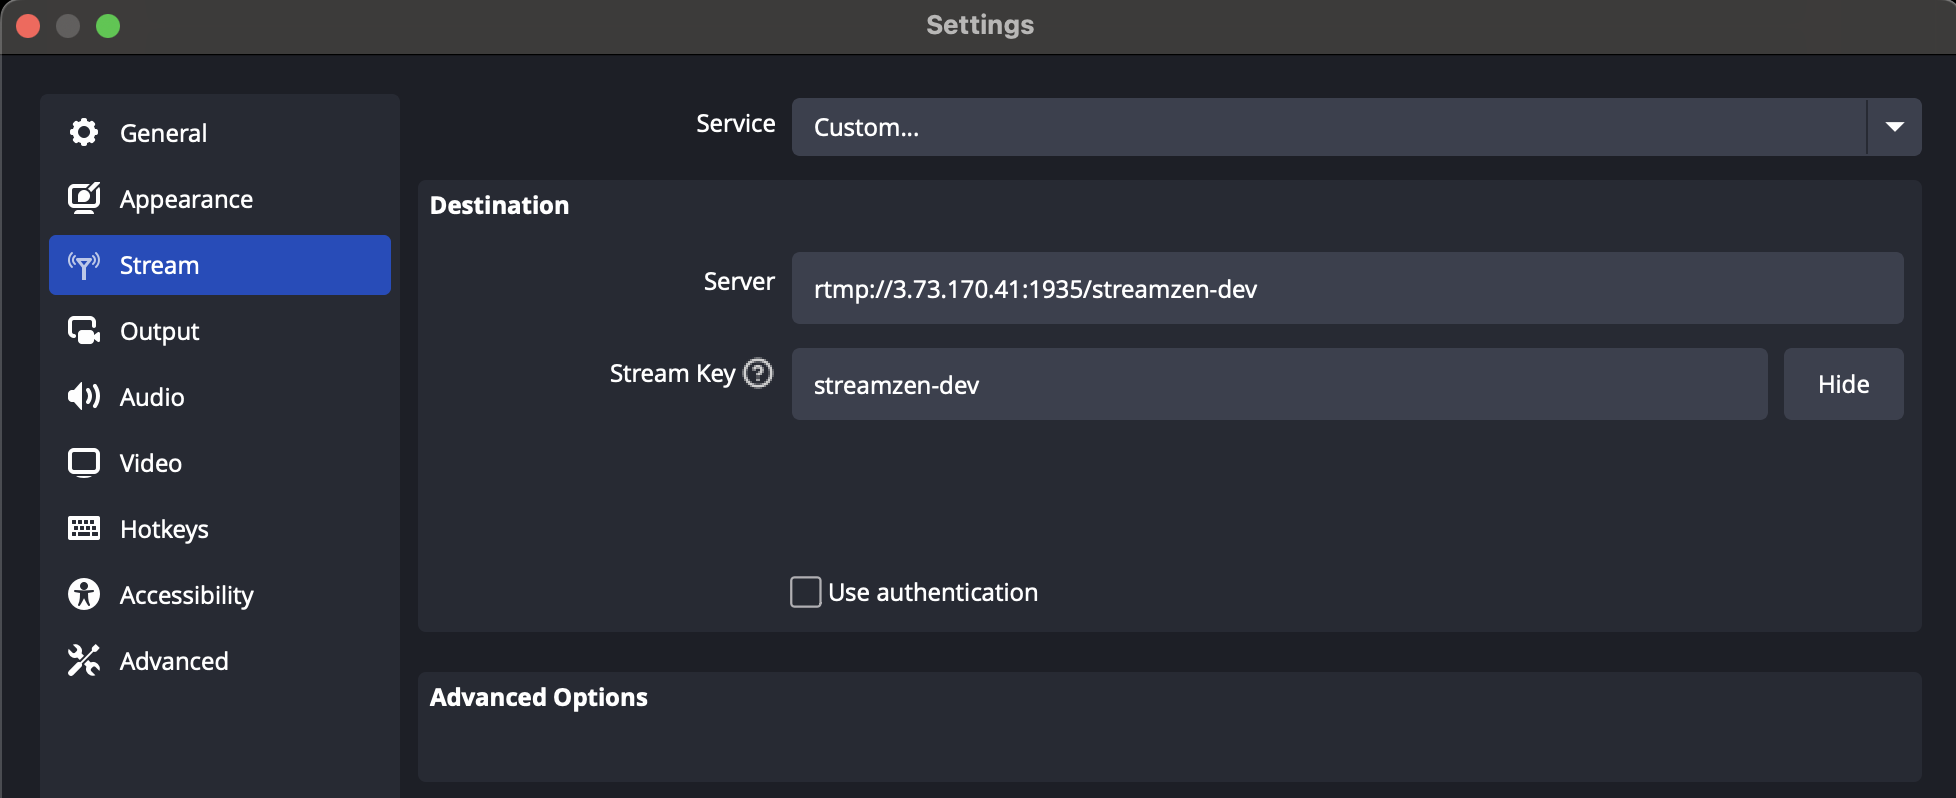
\includegraphics[width=150mm, keepaspectratio]{figures/obs.png}
  \caption{Képernyőkép az OBS stream beállításairól.}
  \label{fig:obs}
\end{figure}

\chapter{Rétegeken átívelő szolgáltatások implementációja}

Ebben a fejezetben kerül kifejtésre az implementációja két szolgáltatásnak az alkalmazásban, amelyek a kliens és szerver rétegén átívelnek: a Single Sign-On (SSO) integrációja és a videófeltöltés folyamata.

\section{Single Sign-On integrációja}

A videók feltöltésére azok jogosultak, akik a stúdióba be tudnak lépni a \verb|/studio| aloldalon, a bejelentkeztetéshez pedig a kari hallgatói közösségünk által nyílt forráskóddal fejlesztett AuthSCH nevű SSO-rendszert integráltam be a weboldalba, ennek az esszenciális tokenkezelési implementációs részeit a backendre bíztam, a kliensoldal csupán a megfelelő útvonalakra irányításért felel.

\Az+\ref{lst:authCtx}. kódrészlet mutatja be a React-alkalmazásban használt \verb|AuthCtx| nevű kontextust, amely JSON Web Tokeneket (JWT)\cite{jwt} használ a bejelentkeztetés során a felhasználói adatok biztonságos és állapotmentes átpasszolására. A \verb|useMe| nevű hook a backend \verb|/api/auth/me| végpontjáról kéri le a bejelentkezett felhasználó adatait, a végpont mögötti logika csupán annyiból áll, hogy kibontja a kódolt JWT-t és visszaadja abból a releváns profiladatokat. Az \verb|AuthProvider| nevű React-függvénykomponens biztosítja a kontextust az alkalmazás többi részének, a \verb|useAuth| hookon keresztül lehet indítani a többi komponensekben bejelentkezést és kijelentkezést (\verb|login| és \verb|logout| függvények), lehet megtudni, van-e bejelentkezett felhasználó a rendszerben (\verb|authenticated| boolean változó).

\begin{minipage}{0.92\textwidth}
  \begin{lstlisting}[
  caption=auth-context.tsx fájl tartalma.,
  label=lst:authCtx,
  style=js,
  basicstyle=\fontsize{10}{12}\ttfamily
]
import { createContext, PropsWithChildren } from "react"
import { useMe } from "./use-me.hook"

type AuthCtxType = {
  authenticated: boolean
  isLoading: boolean
  login: () => void
  logout: () => void
}
export const AuthCtx = createContext<AuthCtxType | undefined>(undefined)

export function AuthProvider({ children }: PropsWithChildren) {
  const { data, isLoading } = useMe()
  const onLogin = async () => {
    window.location.href = import.meta.env.VITE_BACKEND_URL+"/auth/login"
  }
  const onLogout = async () => {
    window.location.href = import.meta.env.VITE_BACKEND_URL+"/auth/logout"
  }
  const value = {
    authenticated: !!data,
    isLoading,
    login: onLogin,
    logout: onLogout,
  }
  return <AuthCtx.Provider value={value}>{children}</AuthCtx.Provider>
}
export function useAuth() {
  const context = useContext(AuthContext)
  if (context === undefined) {
    throw new Error("useAuth must be used within an AuthProvider")
  }
  return context
}
\end{lstlisting}
\end{minipage}

A szerver oldalán egy \verb|AuthModule| névre hallgató NestJS-modul került létrehozásra, amely a \verb|AuthController| és \verb|AuthService| osztályokat tartalmazza. Az \verb|AuthController| osztályban kerülnek definiálásra a forgalmat lehallgató HTTP-végpontok/függvények, míg az \verb|AuthService| osztály elkülöníti a konkrét üzleti logikát. \Az+\ref{lst:authController}. kódrészlet bemutat két fontos HTTP-végpontot, a \verb|/api/auth/login| és a \verb|/api/auth/callback| útvonalakon GET metódusra hallgatókat sorrendben.

\begin{minipage}{0.92\textwidth}
  \begin{lstlisting}[
    caption=Az AuthController osztály fontos függvényei.,
    label=lst:authController,
    style=js,
    basicstyle=\fontsize{10}{12}\ttfamily
  ]
@UseGuards(AuthSchGuard)
@Get("login")
@ApiFoundResponse({
  description: "Redirects to the AuthSch login page.",
})
login() {}

@Get("callback")
@UseGuards(AuthSchGuard)
@ApiFoundResponse({
  description: "Redirects to the frontend and sets cookie with JWT.",
})
@ApiQuery({ name: "code", required: true })
oauthRedirect(@CurrentUser() user: UserDto, @Res() res: Response): void {
  const jwt = this.authService.login(user)
  res.cookie("jwt", jwt, {
    httpOnly: true,
    secure: true,
    domain: process.env.NODE_ENV === "production" ? getHostFromUrl(process.env.FRONTEND_CALLBACK) : undefined,
    maxAge: 1000 * 60 * 60 * 24 * 7, // 7 days
  })
  res.redirect(302, process.env.FRONTEND_CALLBACK + "?authenticated=true")
}
\end{lstlisting}
\end{minipage}

A \verb|AuthSchGuard| egy NestJS-dekorátor, amely fel kell kerüljön a \verb|oauthRedirect| és \verb|login| függvényekre. E mögött a dekorátor mögött egy Passport.js-stratégia\cite{passport} van, amely megvalósítja az AuthSCH-val való OAuth-alapú beazonosítási logikát az OAuth-token megújítását, ehhez kell beállítja a kapott OAuth-kliens azonosítóját és titkos kulcsát, ezen értékek forrásáról később \az+\ref{sec:envvars}. alfejezet beszél.

A \verb|login| függvényt maga az \verb|AuthSchGuard| dekorátor kiváltja, a függvény törzsébe nem kell semmit se írni, a mögöttes logika a felhasználót átirányítja az AuthSCH bejelentkezési oldalára. Az \verb|oauthRedirect| függvény a sikeres bejelentkezés után visszairányítja a~felhasználót a frontendre, a kérésben a \verb|jwt| nevű HTTP-only biztonságos sütit beállítja\cite{ietf-oauth-security-topics-13}, amely tartalmazza a bejelentkezett felhasználóra jellemző JWT-t 7 napos lejárati idővel. A \verb|@CurrentUser()| dekorátor a bejelentkezett felhasználó adatait injektálja a megadott \verb|user| paraméterbe (ezt az \verb|AuthSchGuard| oldja meg a háttérben, kiolvassa a~kapott autorizációs kódot, amit az AuthSCH-tól kapott). Az \verb|AuthService| osztály \verb|login| függvénye a bejelentkezett AuthSCH-s felhasználó adatait kapja meg, amelyből a JWT-t generálja, ezt \az+\ref{lst:authService}. kódrészlet mutatja be. A \verb|createOrUpdateUser| függvény a Prisma ORM segítségével megkeresi a felhasználót az adatbázisban, ha nem találja, akkor létrehozza azt, ha megtalálja, akkor frissíti a felhasználó adatait, ez a függvény kerül felhasználásra az \verb|AuthSchGuard| mögötti stratégiában is a bejelentkeztetés validációs ``mellékhatásaként'', hogy a saját adatbázisunkban is létrejöjjön a felhasználó.

\begin{minipage}{0.92\textwidth}
  \begin{lstlisting}[
    caption=Az AuthService osztály fontos függvényei.,
    label=lst:authService,
    style=js,
    basicstyle=\fontsize{10}{12}\ttfamily
  ]
login(user: object): string {
  return this.jwtService.sign(user, {
    secret: this.configService.get<string>("JWT_SECRET"),
    expiresIn: "7 days",
  })
}
async createOrUpdateUser(prof: AuthSchProfile): Promise<UserDto> {
  const gravatarUrl = this.getGravatarUrl(prof.email, 200)
  return this.prisma.user.upsert({
    where: { authSchId: prof.authSchId },
    update: {
      fullName: prof.fullName,
      firstName: prof.firstName,
      email: prof.email,
      imageUrl: gravatarUrl,
    },
    create: {
      authSchId: prof.authSchId,
      fullName: prof.fullName,
      firstName: prof.firstName,
      email: prof.email,
      imageUrl: gravatarUrl,
    },
  })
}
\end{lstlisting}
\end{minipage}

Lefejlesztésre került egy másik \emph{guard} típusú NestJS-dekorátor, ez a \verb|JwtGuard|, amelyet minden más a szerveren található végpontra be kell vezetni, amennyiben az bejelentkezett felhasználót igényel, ez a dekorátor ellenőrzi a \verb|jwt| süti jelenlétét, a felhasználót beazonosítja. Az ilyen függvényekben is, ha a paraméterre egy \verb|@CurrentUser()| dekorátort helyezünk, akkor a felhasználó adatai automatikusan be lesznek injektálva abba a~paraméterbe.

\section{Videófeltöltés folyamata}

A videófeltöltés lehetőségét helyileg a stúdió aloldalán videóprojekt létrehozása után a~szerkesztőmódban találhatjuk meg, a feltöltésre egy ``dropzone'' került implementálásra, amely egy olyan input mező, amely képes lekezelni ``drag\'n\'drop'' (magyarul \emph{fogd és vidd}) módszerrel ráejtett fájlokat, azt felküldeni a szervernek. Ennek kódjából mutat be részletet \az+\ref{lst:dropzone}. kódrészlet.

\begin{minipage}{0.92\textwidth}
  \begin{lstlisting}[
    caption=Részlet a Dropzone függvénykomponensből.,
    label=lst:dropzone,
    style=js,
    basicstyle=\fontsize{10}{12}\ttfamily
  ]
export const Dropzone = ({ onChange, ...props }) => {
  const fileInputRef = useRef<HTMLInputElement | null>(null)
  // ...
  const handleDrop = (e) => {
    e.preventDefault()
    e.stopPropagation()
    const { files } = e.dataTransfer
    handleFiles(files)
  }
  const handleFileInputChange = (e) => {
    const { files } = e.target
    if (files) handleFiles(files)
  }
  const handleFiles = (files: FileList) => {
    onChange(() => Array.from(files))
    // ...
  }
  const handleButtonClick = () => {
    fileInputRef.current?.click()
  }
  return (
    <Card ... onClick={handleButtonClick}>
      <CardContent ... onDragOver={handleDragOver} onDrop={handleDrop}>
        <div className="...">
          <span className="font-medium">Húzz egy fájlt ide</span>
          <Button variant="ghost" size="sm" className="...">
            vagy kattints ide
          </Button>
          <input ref={fileInputRef} type="file" onChange={handleFileInputChange} className="hidden" multiple />
        </div>
      </CardContent>
    </Card>
  )
}
\end{lstlisting}
\end{minipage}

A \verb|Dropzone| nevű React-függvénykomponens maga az input mező egy rejtett HTML-elem, amely a \verb|fileInputRef| referencián keresztül érhető el. A fájlok feltöltésére a~\verb|handleFiles| függvény felelős, amely a kiválasztott fájlokat egy tömbbé alakítja, és kihív a paraméterben átadott \verb|onChange| függvényre a szülőkomponensben. A konkrét szerver felé kommunikálást a szülőkomponens végzi.

Feltöltés végeztével a szerkesztői felületen megjelenik a ``Videó megtekintése'' gomb, amelyre kattintva elnavigál a weboldal egy új aloldalra, ahol a videólejátszó is implementálásra került. A videólejátszó komponens a \verb|VideoPlayer| nevű React-függvénykomponens, amely a \verb|hls.js| nevű könyvtárat használja a stream letöltés kezelésére. \Az+\ref{lst:videoPlayer}. kódrészlet mutatja be a könyvtár használatát, a komponens implementációját.

\begin{minipage}{0.92\textwidth}
  \begin{lstlisting}[
    caption=A VideoPlayer függvénykomponens kódja.,
    label=lst:videoPlayer,
    style=js,
    basicstyle=\fontsize{10}{12}\ttfamily
  ]
import Hls from "hls.js"
import { useEffect } from "react"

export const VideoPlayer = ({ src, width, height }) => {
  const ref = React.useRef<HTMLVideoElement>(null)
  useEffect(() => {
    if (ref.current && Hls.isSupported()) {
      const hls = new Hls()
      hls.loadSource(src)
      hls.attachMedia(ref.current)
    }
  }, [src])
  return (
    <video width={width} height={height} controls ref={ref}>
      <source src={src} type="video/mp4" />
      Your browser does not support the video tag.
    </video>
  )
}
\end{lstlisting}
\end{minipage}

A szerveroldalon a feltöltésre kerülő nyers videók egy arra kijelölt S3-vödörbe kerülnek továbbításra. A korábban ismertetett (\ref{sec:nodejs}. alfejezet) videókért felelős NestJS-modulbeli \verb|VideoController| és \verb|VideoService| osztályokból emeli ki rendre \az+\ref{lst:videoController}. kódrészlet és \az+\ref{lst:videoService} kódrészlet a fontosabb részeket.

\begin{minipage}{0.92\textwidth}
  \begin{lstlisting}[
    caption=Videófeltöltés kezelése a VideoController osztályban.,
    label=lst:videoController,
    style=js,
    basicstyle=\fontsize{10}{12}\ttfamily
  ]
@Post(":id/upload")
@UseGuards(JwtGuard)
@UseInterceptors(FileInterceptor("file"))
async upload(
  @Param("id") id: string,
  @UploadedFile(new ParseFilePipe()) file: Express.Multer.File
) {
  const { originalname, buffer } = file
  const res = await this.videoService.upload(id, originalname, buffer)
  return await this.videoService.afterUpload(id, res.fileName)
}
\end{lstlisting}
\end{minipage}

A feltöltéshez szükséges fájlok a kliensoldalon kerülnek kiválasztásra, és a POST metódusú \verb|/api/videos/:id/upload| végponton keresztül kerülnek feltöltésre. Ezt a végpontot hallgatja le a \verb|VideoController| osztálybéli \verb|upload| függvény is. A függvény dekorátorai közül a \verb|@Post| jelöli azt, amiképp hallgat a kérésekre (POST metódussal és a jelölt útvonalon). A \verb|@UseGuards| dekorátor az autentikáció szükségességét biztosítja a kérések végbemeneteléhez, amelyet a mi esetünkben a \verb|JwtGuard| osztály valósít meg. A \verb|@UseInterceptors| dekorátor pedig egy interceptort állít be a függvény elé, a fájlok feltöltését segíti elő, amelyet a \verb|FileInterceptor| osztály valósít meg. Ez az osztály a NestJS alatt működő Express keretrendszerben működő \emph{Multer} nevű Node.js-middleware-t hasznosítja, amellyel így tehát képes az osztály mögötti logika a HTTP-alapú bájtfolyamot hatékonyan feldolgozni/parse-olni, és elrejteni előlünk a sok-sok kihívását egy fájlfeltöltésnek. A függvény paramétereiben a \verb|file| paraméter a \verb|@UploadedFile| dekorátoron keresztül válik a feltöltött fájl reprezentációjává, típusa is a \verb|File| interfész lesz.

A \verb|VideoService|-ben működő \verb|upload| függvény felé lesz a kapott fájl bufferje továbbítva, végül a service függvény eredményéből született fájlnévvel kerül az adatbázisba is lementésre az entitásként a videó is a \verb|afterUpload| függvény által.

A \verb|VideoService| az AWS SDK S3 API-ját használja a fájlok vödörbe való feltöltésére. Ehhez létrehoztam tagváltozóként a \verb|s3Client|-et. Az \verb|upload| függvény először átalakítja a fájlnevet, megtartja a kiterjesztést, viszont a dátumot szerkeszti bele a konkrét névbe. Majd pedig készít egy \verb|PutObjectCommand| típusú objektumot, amellyel a megfelelő helyre és névvel kerül feltöltésre az \verb|s3Client|-en keresztül a fájl.

\begin{minipage}{0.92\textwidth}
  \begin{lstlisting}[
    caption=Videófeltöltés függvénye a VideoService osztályban.,
    label=lst:videoService,
    style=js,
    basicstyle=\fontsize{10}{12}\ttfamily
  ]
private readonly s3Client = new S3Client({
  region: this.configService.getOrThrow("AWS_S3_REGION"),
})
async upload(id: string, fileName: string, file: Buffer) {
  const ext = fileName.split(".").slice(-1)[0]
  const baseName = new Date()
    .toISOString().slice(0, 19).replaceAll(":", "-")

  const response = await this.s3Client.send(
    new PutObjectCommand({
      Bucket: this.configService.getOrThrow("AWS_S3_UPLOADED_BUCKET"),
      Key: `${id}/${baseName}.${ext}`,
      Body: file,
    })
  )
  return { ...response, fileName: `${baseName}.${ext}` }
}
\end{lstlisting}
\end{minipage}

\chapter{Elkészült funkciók tesztelése}

\section{Live streaming tesztelése}

A weboldalamon a \verb|/live| útvonalon megtekintettem az előzőleg (\ref{sec:mediaLive}. alfejezet) beindított streamet (\refstruc{fig:waterfall1}). Egy próbálkozást mutat be \az+\refstruc{fig:waterfall2} által bemutatott képernyőkép, amely a~böngészőben a HTTP-kérések vízesését\cite{waterfall} mutatja be.

\begin{figure}[h]
  \centering
  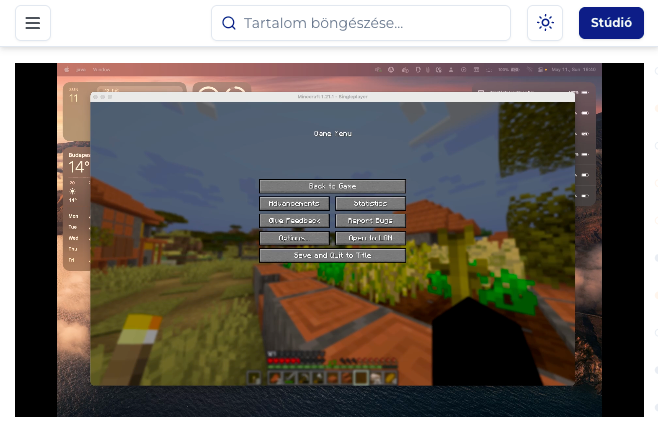
\includegraphics[width=100mm, keepaspectratio]{figures/waterfall1.png}
  \caption{A /live útvonalon látható aloldal.}
  \label{fig:waterfall1}
\end{figure}

\begin{figure}[h]
  \centering
  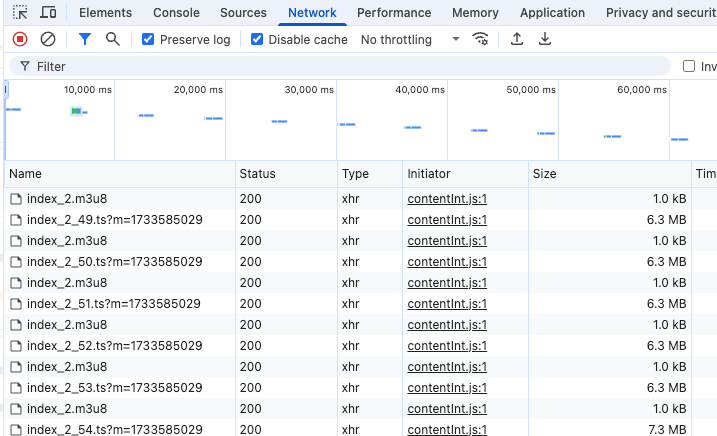
\includegraphics[width=100mm, keepaspectratio]{figures/waterfall2.png}
  \caption{HTTP-kérések vízesése a /live oldalon.}
  \label{fig:waterfall2}
\end{figure}

Az SPA-alkalmazás a környezeti változóból beállított HLS-végponton kéri le először a~\verb|.m3u8| playlistet, amelyből megtudja, mi lesz a következő szegmens, amit le kell töltsön. Az ábrából látszik, hogy az alapértelmezett 6 másodperces részekre vannak felbontva a~szegmensek. Nagyjából 6--7 MB-os szegmensek érkeznek a böngészőbe (már tömörítve a~CDN-en keresztül).

A MediaPackage v2-es verziója támogatja a Low Latency HLS (LL-HLS) alapú streamelést is, azonban én még a v1-es verziót használtam és a kliensoldali implementációs is meghagytam a hagyományos HLS-en. A fent ismertetett élő stream MediaLive és MediaPackage közti integrációjának manuális tesztelése folyamán körülbelül 10 másodperces késleltetéssel láttam a böngészőben azt, amit a másik képernyőn csináltam.

Teljesítmény szempontjából a fenti streamelés késleltetését két dolog befolyásolja jelentősen: a kódolási beállítások (mekkora szegmensekre bontsa, hányféle kimenet legyen, milyen hibaaránnyal érkezik a forrásvideó) és a lejátszó bufferelési logikája. Előbbi befolyásoló tényezőnek a mögöttes forrása a MediaLive maga, ami a kódolást intézi. Mind a~MediaLive és a MediaPackage menedzselt szolgáltatások, magunk nem tudunk hatással lenni az azalatti erőforrások eloszlására, annak növelésére, ugyanis automatikusan skálázódnak, ahogy arra a szolgáltatás elköteleződik is.

A késleltetés mérésére a nézők számának növelésével nem tudnánk hasznos teljesítményteszteket készíteni, a live betöltődik a MediaLive-ba, utána a kész szegmensek kiszórása az, ami kihívás a rendszer számára, viszont -- ahogy ezt fentebb kifejtettem -- a~MediaPackage automatikusan skálázódással oldja meg ezt bizonyos kvótákig -- például egy HLS-végponton másodpercenként 300 kérést tud befogadni\cite{empQuotas} --, de még ennek a terhelését is hívatott megvédeni megfelelő gyorsítótárazással egy CDN. Csupán abban az esetben érheti teljesítményromlás a rendszert, ha a MediaPackage hatáskörén kívül magára az AWS hálózatára fejtenek ki jelentős terhelést a végfelhasználók.\cite{latency}

\section{VOD streaming tesztelése}\label{sec:vod_test}

A MediaConvert-jobot bemutató \ref{sec:jobStarter}. alfejezet vége korábban bemutatta egy videófeltöltés utáni VOD streaming tesztelését különféle sávszélekkel kísérletezve. Jelen szekció ezt továbbviszi, és leteszteli milyen számokat ad ki a folyamat, ha nem a sávszéllel, hanem a videók edge-re való közelebbhozásával kísérletezünk.

A VOD streameket közvetlen S3-ból szolgáljuk ki. A technológiai ismertető (\ref{sec:aws_elemental}. alfejezet) is referált már rá, korábban a videók tárolására a széleskörű kiszolgálásra korábban létezett szolgáltatás, azonban ezt kiváltotta az S3.\cite{Mediastore} Az S3 szintén fel van készítve a skálázódásra\cite{s3perf}, így nem szükséges aggódni, viszont a kiszolgálás késleltetését érdemes csökkenteni úgy, hogy az edge rétegén gyorsítótárazást valósítunk meg, ezt persze CDN-nel. A CloudFront cache beállításaival való kísérletezésre összeállítottam egy tesztkörnyezetet, amelyben a CDN cache beállításait variálva figyeltem meg a válaszidőket. A teszteléshez a \emph{Grafana k6}-ot\footnote{\url{https://k6.io/}} használtam, amelynek segítségével a válaszidőket és a válaszok méretét is tudtam mérni.\cite{loadtests}

Nyilván egy 1 éves caching policy bekapcsolásával a \verb|/media-assets| elérési útvonalra érkező kérések válaszideje csökkent, hiszen az adatok a CDN gyorsítótárából, konkrétan a~budapesti edge szerverfarmról érkeztek, nem pedig közvetlenül az S3-ból, amely a~frankfurti adatközpontban lakik. A tesztelés alatt 100 virtuális felhasználó egy megadott kétperces ablakban alatt szórt felhasználónként 20 kérést, vegyesen kérték le egy videó szegmenseit. A szkript kódját mutatja be \az+\ref{lst:k6}. kódrészlet. A tesztelés során cache nélkül a válasz megérkezésére a várakozási idő az esetek 90\%-ában 226,59 ms vagy azalatti volt, míg ugyanez a cache beállítással 177,39 ms vagy azalatti volt.

\begin{minipage}{0.92\textwidth}
  \begin{lstlisting}[
    caption=A k6 tesztelő szkript kódja.,
    label=lst:k6,
    style=tf,
    basicstyle=\fontsize{10}{12}\ttfamily,
  ]
export const options = {
  scenarios: {
    contacts: {
      executor: 'per-vu-iterations',
      vus: 100,
      iterations: 20,
      maxDuration: '2m',
    },
  },
};
const basePath = "https://stream.trisz.hu/media-assets";
const videoPath = basePath + "/cmajngfey0005hadzcbli5k2c/2025-05-11T12-48-43.mp4_1080p_";

export default function() {
  const n = Math.floor(Math.random() * 11) + 1; // 1-11
  const res = http.get(videoPath + String(n).padStart(5, '0') + '.ts');
  check(res, {
    'is status 200': (r) => r.status === 200,
    'is loaded': (r) => r.body.length > 0,
    'is cached': (r) => r.headers['X-Cache'] === 'Hit from cloudfront',
  });
}  
\end{lstlisting}
\end{minipage}

\chapter{Összegzés}

A streaming rendszereket kiszolgáló technológiák fejlődése közel sem ért véget, a QUIC protokoll -- és az arra épülő Media over QUIC\cite{ietf-moq-transport-11} (MoQ) -- előretörésével, új modern CDN-funkcionalitásokkal\cite{openconnect}, a szerverfarmokban használt alkalmazásspecifikus chipek fejlődésével, illetve hatékonyabb kodekek megjelenésével egyre magasabb minőséget lehet szolgáltatni. Az általam bemutatott rendszer egy egyszerűsített példája a streaming rendszereknek, amely lehetőséget ad arra, hogy megértsük a mögöttes technológiákat és azok működését, betekintést nyújt néhány tipikusan streamingre használt AWS-erőforrás világába, a~tervezési technikák palettájába.

A fejlesztés ideje alatt ahogy egyre több komponenst kötöttem a rendszerbe, úgy nőtt a felhőszolgáltatások költsége is. A dolgozat írásához többször újrateszteltem a futó rendszert, a márciusi összköltsége AWS-ben \$67.98 lett, áprilisban \$73.29, ezekben az összegekben a~legjelentősebbek közé tartozott az RDS-adatbázis (\$14--\$17 között), az ALB-példány (\$17--\$20 között) és az ECS-klaszter (\$10--\$11 között) költsége, ezek nem on-demand jellegűek. Pár szolgáltatás (Lambda, CloudWatch Logs) pedig a \emph{free tier}, azaz ingyenes átkategóriában tudott maradni. Májusra a Cost Management \$78-t jelzett előre, a hónapban végzett k6 tesztelés próbálgatása miatti (\ref{sec:vod_test}. alfejezet) kb. 100 GB CloudFront-forgalom se emelte jobban.

\section{Továbbfejlesztés lehetőségei}

Architekturális szempontból a webszerver átszervezhető mikroszolgáltatásos alapokra, amennyiben a jövőben a rendszer bővítése, új funkciók bevezetése indokolttá teszi, ezzel is jobban támogatva a már megkezdett event-driven architecture (EDA)\cite{eda} irányvonalat.

Biztonság szempontjából a rendszer továbbfejlesztése érdekében érdemes lenne megfontolni a naplózást kiterjeszteni a CDN és a WAF szintjén ``access loggingra'' is, a VPC-n belül a Flow logok bekapcsolására. Élő, nagy forgalmú rendszerben kihagyhatatlan kötelességünk volna a WAF ACL-ben foglalt szabályokat finomhangolni veszélyes forgalom kiszűrésére. \Az+\ref{sec:vpc}.~alfejezetben említett NAT Gateway és VPC Endpoint megoldások alkalmazása is javallott volna.

A kiszolgálás minőségének javítására érdemes lehet akár a CloudFront-disztribúció cache beállításait is optimalizálás szempontjából újraszemlézni. Felmerülhet egy nagyobb rendszernél a webszerver felé irányított forgalom hálózati terheléséből származó kihívásokra felkészíteni az ALB-példányt is, erre lehet igénybe venni Load balancer Capacity Unit (LCU) foglalást, amely biztosít megfelelő számítási kapacitást a forgalom fogadására. Emellett az ECS-klaszterbe is be lehet vezetni egy automatikus skálázási megoldást, amely a forgalom növekedésével automatikusan új taszkokat indít el az ECS-szolgáltatásban, ezzel biztosítva a megfelelő számítási kapacitást.

A rendszer erős kódmigrálást, infrastruktúra-átalakítást igényelne, amennyiben cél volna a \emph{vendor lock-in}\cite{lockIn} kockázatainak mitigálása. Ehhez javasolt lenne a Kubernetesre\footnote{\url{https://kubernetes.io/}} való áttérés ECS-ről\cite{k8s}, Ceph\footnote{\url{https://ceph.io/en/}} használata S3 helyett, a Kubernetes alá hozható az~adatbázis, illetve a Lambda-függvények is kis mikroszolgáltatások formájában. A~MediaConvert, a~MediaLive és MediaPackage szolgáltatások kiváltása már bonyolultabb lehet, ebben segíthet az általam korábbi projektben megismert FFMpeg és az NGINX RTMP\leavevmode\hbox{-}modulja\cite{rtmpNginx}, ahogy azt \az+\ref{sec:elso_lepesek} alfejezetben is említettem.

Nem utolsó sorban a live streaming kiterjesztése még egy feladat, ami várat magára. A rendszer jelenleg nem engedi több élő adás indítását, ezt lehetne kiterjeszteni kódból történő dinamikus MediaLive- és MediaPackage-csatornák felkonfigurálására.


% %----------------------------------------------------------------------------
\chapter*{\koszonetnyilvanitas}\addcontentsline{toc}{chapter}{\koszonetnyilvanitas}
%----------------------------------------------------------------------------

Ez nem kötelező, akár törölhető is. Ha a szerző szükségét érzi, itt lehet köszönetet nyilvánítani azoknak, akik hozzájárultak munkájukkal ahhoz, hogy a hallgató a szakdolgozatban vagy diplomamunkában leírt feladatokat sikeresen elvégezze. A konzulensnek való köszönetnyilvánítás sem kötelező, a konzulensnek hivatalosan is dolga, hogy a hallgatót konzultálja.
%\listoffigures\addcontentsline{toc}{chapter}{\listfigurename}
%\listoftables\addcontentsline{toc}{chapter}{\listtablename}
\addcontentsline{toc}{chapter}{\bibname}
\bibliography{bib/mybib}
% %----------------------------------------------------------------------------
\appendix
%----------------------------------------------------------------------------
\chapter*{\fuggelek}\addcontentsline{toc}{chapter}{\fuggelek}
\setcounter{chapter}{\appendixnumber}
%\setcounter{equation}{0} % a fofejezet-szamlalo az angol ABC 6. betuje (F) lesz
\numberwithin{equation}{section}
\numberwithin{figure}{section}
\numberwithin{lstlisting}{section}
%\numberwithin{tabular}{section}

%----------------------------------------------------------------------------
\section{A TeXstudio felülete}
%----------------------------------------------------------------------------
\begin{figure}[!ht]
\centering
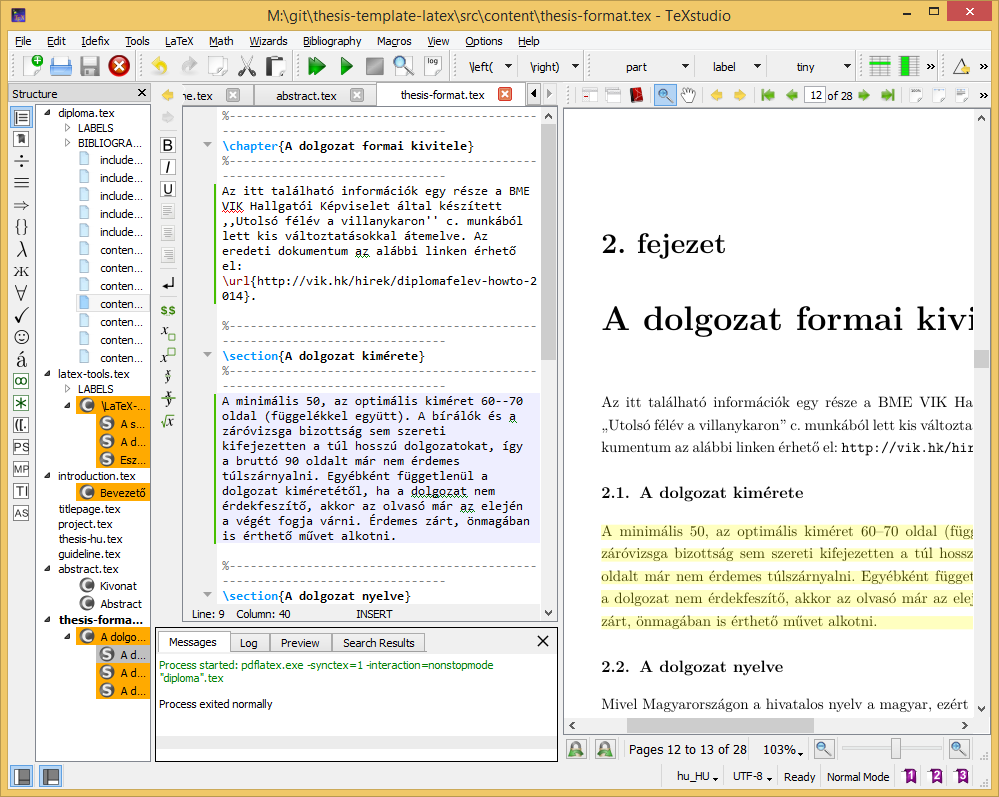
\includegraphics[width=150mm, keepaspectratio]{figures/TeXstudio.png}
\caption{A TeXstudio \LaTeX-szerkesztő.} 
\end{figure}

%----------------------------------------------------------------------------
\clearpage\section{Válasz az ,,Élet, a világmindenség, meg minden'' kérdésére}
%----------------------------------------------------------------------------
A Pitagorasz-tételből levezetve
\begin{align}
c^2=a^2+b^2=42.
\end{align}
A Faraday-indukciós törvényből levezetve
\begin{align}
\rot E=-\frac{dB}{dt}\hspace{1cm}\longrightarrow \hspace{1cm}
U_i=\oint\limits_\mathbf{L}{\mathbf{E}\mathbf{dl}}=-\frac{d}{dt}\int\limits_A{\mathbf{B}\mathbf{da}}=42.
\end{align}


\label{page:last}
\end{document}
